\documentclass[a4paper]{book}
\usepackage{a4wide}
\usepackage{makeidx}
\usepackage{fancyhdr}
\usepackage{graphicx}
\usepackage{multicol}
\usepackage{float}
\usepackage{textcomp}
\usepackage{alltt}
\usepackage{doxygen}
\makeindex
\setcounter{tocdepth}{1}
\renewcommand{\footrulewidth}{0.4pt}
\begin{document}
\begin{titlepage}
\vspace*{7cm}
\begin{center}
{\Large Open\-RTM Reference Manual\\[1ex]\large 0.2 }\\
\vspace*{1cm}
{\large Generated by Doxygen 1.4.1}\\
\vspace*{0.5cm}
{\small Wed Sep 26 17:47:06 2007}\\
\end{center}
\end{titlepage}
\clearemptydoublepage
\pagenumbering{roman}
\tableofcontents
\clearemptydoublepage
\pagenumbering{arabic}
\chapter{Open\-RTM Directory Hierarchy}
\section{Open\-RTM Directories}
This directory hierarchy is sorted roughly, but not completely, alphabetically:\begin{CompactList}
\item \contentsline{section}{rtm}{\pageref{dir_000000}}{}
\begin{CompactList}
\item \contentsline{section}{idl}{\pageref{dir_000001}}{}
\end{CompactList}
\end{CompactList}

\chapter{Open\-RTM Namespace Index}
\section{Open\-RTM �l�[���X�y�[�X�ꗗ}
�l�[���X�y�[�X�̈ꗗ�ł��B\begin{CompactList}
\item\contentsline{section}{{\bf \_\-\_\-init\_\-\_\-} (Module \char`\"{}\_\-\_\-init\_\-\_\-\char`\"{} )}{\pageref{namespace____init____}}{}
\item\contentsline{section}{{\bf Buffer\-Base} }{\pageref{namespaceBufferBase}}{}
\item\contentsline{section}{{\bf Config\-Admin} }{\pageref{namespaceConfigAdmin}}{}
\item\contentsline{section}{{\bf Corba\-Consumer} }{\pageref{namespaceCorbaConsumer}}{}
\item\contentsline{section}{{\bf Corba\-Naming} }{\pageref{namespaceCorbaNaming}}{}
\item\contentsline{section}{{\bf Corba\-Object\-Manager} }{\pageref{namespaceCorbaObjectManager}}{}
\item\contentsline{section}{{\bf Corba\-Port} }{\pageref{namespaceCorbaPort}}{}
\item\contentsline{section}{{\bf Data\-Flow\-Component\-Base} }{\pageref{namespaceDataFlowComponentBase}}{}
\item\contentsline{section}{{\bf Data\-In\-Port} }{\pageref{namespaceDataInPort}}{}
\item\contentsline{section}{{\bf Data\-Out\-Port} }{\pageref{namespaceDataOutPort}}{}
\item\contentsline{section}{{\bf Default\-Configuration} }{\pageref{namespaceDefaultConfiguration}}{}
\item\contentsline{section}{{\bf ECFactory} }{\pageref{namespaceECFactory}}{}
\item\contentsline{section}{{\bf Execution\-Context\-Base} }{\pageref{namespaceExecutionContextBase}}{}
\item\contentsline{section}{{\bf Ext\-Trig\-Execution\-Context} }{\pageref{namespaceExtTrigExecutionContext}}{}
\item\contentsline{section}{{\bf Factory} }{\pageref{namespaceFactory}}{}
\item\contentsline{section}{{\bf In\-Port} }{\pageref{namespaceInPort}}{}
\item\contentsline{section}{{\bf In\-Port\-Consumer} }{\pageref{namespaceInPortConsumer}}{}
\item\contentsline{section}{{\bf In\-Port\-Corba\-Consumer} }{\pageref{namespaceInPortCorbaConsumer}}{}
\item\contentsline{section}{{\bf In\-Port\-Corba\-Provider} }{\pageref{namespaceInPortCorbaProvider}}{}
\item\contentsline{section}{{\bf In\-Port\-Provider} }{\pageref{namespaceInPortProvider}}{}
\item\contentsline{section}{{\bf Listener} }{\pageref{namespaceListener}}{}
\item\contentsline{section}{{\bf Manager} }{\pageref{namespaceManager}}{}
\item\contentsline{section}{{\bf Manager\-Config} }{\pageref{namespaceManagerConfig}}{}
\item\contentsline{section}{{\bf Module\-Manager} }{\pageref{namespaceModuleManager}}{}
\item\contentsline{section}{{\bf Naming\-Manager} }{\pageref{namespaceNamingManager}}{}
\item\contentsline{section}{{\bf Numbering\-Policy} }{\pageref{namespaceNumberingPolicy}}{}
\item\contentsline{section}{{\bf Object\-Manager} }{\pageref{namespaceObjectManager}}{}
\item\contentsline{section}{{\bf omni\-ORB} }{\pageref{namespaceomniORB}}{}
\item\contentsline{section}{{\bf Out\-Port} }{\pageref{namespaceOutPort}}{}
\item\contentsline{section}{{\bf Out\-Port\-Base} }{\pageref{namespaceOutPortBase}}{}
\item\contentsline{section}{{\bf Out\-Port\-Consumer} }{\pageref{namespaceOutPortConsumer}}{}
\item\contentsline{section}{{\bf Out\-Port\-Corba\-Consumer} }{\pageref{namespaceOutPortCorbaConsumer}}{}
\item\contentsline{section}{{\bf Out\-Port\-Corba\-Provider} }{\pageref{namespaceOutPortCorbaProvider}}{}
\item\contentsline{section}{{\bf Out\-Port\-Provider} }{\pageref{namespaceOutPortProvider}}{}
\item\contentsline{section}{{\bf Periodic\-Execution\-Context} }{\pageref{namespacePeriodicExecutionContext}}{}
\item\contentsline{section}{{\bf Port\-Admin} }{\pageref{namespacePortAdmin}}{}
\item\contentsline{section}{{\bf Port\-Base} }{\pageref{namespacePortBase}}{}
\item\contentsline{section}{{\bf Port\-Call\-Back} }{\pageref{namespacePortCallBack}}{}
\item\contentsline{section}{{\bf Properties} }{\pageref{namespaceProperties}}{}
\item\contentsline{section}{{\bf Publisher\-Base} }{\pageref{namespacePublisherBase}}{}
\item\contentsline{section}{{\bf Publisher\-Factory} }{\pageref{namespacePublisherFactory}}{}
\item\contentsline{section}{{\bf Publisher\-Flush} }{\pageref{namespacePublisherFlush}}{}
\item\contentsline{section}{{\bf Publisher\-New} }{\pageref{namespacePublisherNew}}{}
\item\contentsline{section}{{\bf Publisher\-Periodic} }{\pageref{namespacePublisherPeriodic}}{}
\item\contentsline{section}{{\bf Ring\-Buffer} }{\pageref{namespaceRingBuffer}}{}
\item\contentsline{section}{{\bf RTCUtil} }{\pageref{namespaceRTCUtil}}{}
\item\contentsline{section}{{\bf RTObject} }{\pageref{namespaceRTObject}}{}
\item\contentsline{section}{{\bf Sdo\-Configuration} }{\pageref{namespaceSdoConfiguration}}{}
\item\contentsline{section}{{\bf Sdo\-Organization} }{\pageref{namespaceSdoOrganization}}{}
\item\contentsline{section}{{\bf Sdo\-Service} }{\pageref{namespaceSdoService}}{}
\item\contentsline{section}{{\bf State\-Machine} }{\pageref{namespaceStateMachine}}{}
\item\contentsline{section}{{\bf String\-Util} }{\pageref{namespaceStringUtil}}{}
\item\contentsline{section}{{\bf System\-Logger} }{\pageref{namespaceSystemLogger}}{}
\item\contentsline{section}{{\bf Timer} }{\pageref{namespaceTimer}}{}
\item\contentsline{section}{{\bf Time\-Value} }{\pageref{namespaceTimeValue}}{}
\item\contentsline{section}{{\bf uuid} }{\pageref{namespaceuuid}}{}
\item\contentsline{section}{{\bf version} }{\pageref{namespaceversion}}{}
\end{CompactList}

\chapter{Open\-RTM Hierarchical Index}
\section{OpenRTM クラス階層}
この継承一覧はおおまかにはソートされていますが、完全にアルファベット順でソートされてはいません。\begin{CompactList}
\item \contentsline{section}{BufferBase}{\pageref{classsource__py_1_1_buffer_base_1_1_buffer_base}}{}
\begin{CompactList}
\item \contentsline{section}{NullBuffer}{\pageref{classsource__py_1_1_buffer_base_1_1_null_buffer}}{}
\end{CompactList}
\item \contentsline{section}{ConfigAdmin}{\pageref{classsource__py_1_1_config_admin_1_1_config_admin}}{}
\item \contentsline{section}{ConfigBase}{\pageref{classsource__py_1_1_config_admin_1_1_config_base}}{}
\begin{CompactList}
\item \contentsline{section}{Config}{\pageref{classsource__py_1_1_config_admin_1_1_config}}{}
\end{CompactList}
\item \contentsline{section}{Configuration\_\-impl}{\pageref{classsource__py_1_1_sdo_configuration_1_1_configuration__impl}}{}
\item \contentsline{section}{Configuration\_\-impl::config\_\-id}{\pageref{classsource__py_1_1_sdo_configuration_1_1_configuration__impl_1_1config__id}}{}
\item \contentsline{section}{Configuration\_\-impl::org\_\-id}{\pageref{classsource__py_1_1_sdo_configuration_1_1_configuration__impl_1_1org__id}}{}
\item \contentsline{section}{Configuration\_\-impl::service\_\-id}{\pageref{classsource__py_1_1_sdo_configuration_1_1_configuration__impl_1_1service__id}}{}
\item \contentsline{section}{CorbaConsumerBase}{\pageref{classsource__py_1_1_corba_consumer_1_1_corba_consumer_base}}{}
\begin{CompactList}
\item \contentsline{section}{CorbaConsumer}{\pageref{classsource__py_1_1_corba_consumer_1_1_corba_consumer}}{}
\end{CompactList}
\item \contentsline{section}{CorbaNaming}{\pageref{classsource__py_1_1_corba_naming_1_1_corba_naming}}{}
\item \contentsline{section}{CorbaObjectManager}{\pageref{classsource__py_1_1_corba_object_manager_1_1_corba_object_manager}}{}
\item \contentsline{section}{CorbaPort}{\pageref{classsource__py_1_1_corba_port_1_1_corba_port}}{}
\item \contentsline{section}{CorbaPort::Consumer}{\pageref{classsource__py_1_1_corba_port_1_1_corba_port_1_1_consumer}}{}
\item \contentsline{section}{CorbaPort::subscribe}{\pageref{classsource__py_1_1_corba_port_1_1_corba_port_1_1subscribe}}{}
\item \contentsline{section}{CorbaPort::unsubscribe}{\pageref{classsource__py_1_1_corba_port_1_1_corba_port_1_1unsubscribe}}{}
\item \contentsline{section}{DataFlowComponentBase}{\pageref{classsource__py_1_1_data_flow_component_base_1_1_data_flow_component_base}}{}
\item \contentsline{section}{DataInPort}{\pageref{classsource__py_1_1_data_in_port_1_1_data_in_port}}{}
\item \contentsline{section}{DataOutPort}{\pageref{classsource__py_1_1_data_out_port_1_1_data_out_port}}{}
\item \contentsline{section}{DataOutPort::subscribe}{\pageref{classsource__py_1_1_data_out_port_1_1_data_out_port_1_1subscribe}}{}
\item \contentsline{section}{ECFactoryBase}{\pageref{classsource__py_1_1_e_c_factory_1_1_e_c_factory_base}}{}
\begin{CompactList}
\item \contentsline{section}{ECFactoryPython}{\pageref{classsource__py_1_1_e_c_factory_1_1_e_c_factory_python}}{}
\end{CompactList}
\item \contentsline{section}{escape\_\-functor}{\pageref{classsource__py_1_1_string_util_1_1escape__functor}}{}
\item \contentsline{section}{ExecutionContextBase}{\pageref{classsource__py_1_1_execution_context_base_1_1_execution_context_base}}{}
\item \contentsline{section}{ExtTrigExecutionContext}{\pageref{classsource__py_1_1_ext_trig_execution_context_1_1_ext_trig_execution_context}}{}
\item \contentsline{section}{ExtTrigExecutionContext::Worker}{\pageref{classsource__py_1_1_ext_trig_execution_context_1_1_ext_trig_execution_context_1_1_worker}}{}
\item \contentsline{section}{FactoryBase}{\pageref{classsource__py_1_1_factory_1_1_factory_base}}{}
\begin{CompactList}
\item \contentsline{section}{FactoryPython}{\pageref{classsource__py_1_1_factory_1_1_factory_python}}{}
\end{CompactList}
\item \contentsline{section}{InPort}{\pageref{classsource__py_1_1_in_port_1_1_in_port}}{}
\item \contentsline{section}{InPortConsumer}{\pageref{classsource__py_1_1_in_port_consumer_1_1_in_port_consumer}}{}
\item \contentsline{section}{InPortCorbaConsumer}{\pageref{classsource__py_1_1_in_port_corba_consumer_1_1_in_port_corba_consumer}}{}
\item \contentsline{section}{InPortCorbaProvider}{\pageref{classsource__py_1_1_in_port_corba_provider_1_1_in_port_corba_provider}}{}
\item \contentsline{section}{InPortProvider}{\pageref{classsource__py_1_1_in_port_provider_1_1_in_port_provider}}{}
\item \contentsline{section}{ListenerBase}{\pageref{classsource__py_1_1_listener_1_1_listener_base}}{}
\begin{CompactList}
\item \contentsline{section}{ListenerFunc}{\pageref{classsource__py_1_1_listener_1_1_listener_func}}{}
\item \contentsline{section}{ListenerObject}{\pageref{classsource__py_1_1_listener_1_1_listener_object}}{}
\end{CompactList}
\item \contentsline{section}{Logbuf}{\pageref{classsource__py_1_1_system_logger_1_1_logbuf}}{}
\item \contentsline{section}{LogStream}{\pageref{classsource__py_1_1_system_logger_1_1_log_stream}}{}
\item \contentsline{section}{Manager}{\pageref{classsource__py_1_1_manager_1_1_manager}}{}
\item \contentsline{section}{Manager::FactoryPredicate}{\pageref{classsource__py_1_1_manager_1_1_manager_1_1_factory_predicate}}{}
\item \contentsline{section}{Manager::InstanceName}{\pageref{classsource__py_1_1_manager_1_1_manager_1_1_instance_name}}{}
\item \contentsline{section}{Manager::OrbRunner}{\pageref{classsource__py_1_1_manager_1_1_manager_1_1_orb_runner}}{}
\item \contentsline{section}{Manager::Term}{\pageref{classsource__py_1_1_manager_1_1_manager_1_1_term}}{}
\item \contentsline{section}{Manager::Terminator}{\pageref{classsource__py_1_1_manager_1_1_manager_1_1_terminator}}{}
\item \contentsline{section}{ManagerConfig}{\pageref{classsource__py_1_1_manager_config_1_1_manager_config}}{}
\item \contentsline{section}{ModuleManager}{\pageref{classsource__py_1_1_module_manager_1_1_module_manager}}{}
\item \contentsline{section}{ModuleManager::DLL}{\pageref{classsource__py_1_1_module_manager_1_1_module_manager_1_1_d_l_l}}{}
\item \contentsline{section}{ModuleManager::Error}{\pageref{classsource__py_1_1_module_manager_1_1_module_manager_1_1_error}}{}
\begin{CompactList}
\item \contentsline{section}{ModuleManager::InvalidArguments}{\pageref{classsource__py_1_1_module_manager_1_1_module_manager_1_1_invalid_arguments}}{}
\item \contentsline{section}{ModuleManager::InvalidOperation}{\pageref{classsource__py_1_1_module_manager_1_1_module_manager_1_1_invalid_operation}}{}
\item \contentsline{section}{ModuleManager::NotAllowedOperation}{\pageref{classsource__py_1_1_module_manager_1_1_module_manager_1_1_not_allowed_operation}}{}
\end{CompactList}
\item \contentsline{section}{ModuleManager::NotFound}{\pageref{classsource__py_1_1_module_manager_1_1_module_manager_1_1_not_found}}{}
\begin{CompactList}
\item \contentsline{section}{ModuleManager::FileNotFound}{\pageref{classsource__py_1_1_module_manager_1_1_module_manager_1_1_file_not_found}}{}
\item \contentsline{section}{ModuleManager::ModuleNotFound}{\pageref{classsource__py_1_1_module_manager_1_1_module_manager_1_1_module_not_found}}{}
\item \contentsline{section}{ModuleManager::SymbolNotFound}{\pageref{classsource__py_1_1_module_manager_1_1_module_manager_1_1_symbol_not_found}}{}
\end{CompactList}
\item \contentsline{section}{NamingBase}{\pageref{classsource__py_1_1_naming_manager_1_1_naming_base}}{}
\begin{CompactList}
\item \contentsline{section}{NamingOnCorba}{\pageref{classsource__py_1_1_naming_manager_1_1_naming_on_corba}}{}
\end{CompactList}
\item \contentsline{section}{NamingManager}{\pageref{classsource__py_1_1_naming_manager_1_1_naming_manager}}{}
\item \contentsline{section}{NamingManager::Comps}{\pageref{classsource__py_1_1_naming_manager_1_1_naming_manager_1_1_comps}}{}
\item \contentsline{section}{NamingManager::Names}{\pageref{classsource__py_1_1_naming_manager_1_1_naming_manager_1_1_names}}{}
\item \contentsline{section}{NumberingPolicy}{\pageref{classsource__py_1_1_numbering_policy_1_1_numbering_policy}}{}
\begin{CompactList}
\item \contentsline{section}{DefaultNumberingPolicy}{\pageref{classsource__py_1_1_numbering_policy_1_1_default_numbering_policy}}{}
\end{CompactList}
\item \contentsline{section}{NumberingPolicy::ObjectNotFound}{\pageref{classsource__py_1_1_numbering_policy_1_1_numbering_policy_1_1_object_not_found}}{}
\item \contentsline{section}{nv\_\-find}{\pageref{classsource__py_1_1_n_v_util_1_1nv__find}}{}
\item \contentsline{section}{ObjectManager}{\pageref{classsource__py_1_1_object_manager_1_1_object_manager}}{}
\item \contentsline{section}{ObjectManager::Objects}{\pageref{classsource__py_1_1_object_manager_1_1_object_manager_1_1_objects}}{}
\item \contentsline{section}{OnOverflow}{\pageref{classsource__py_1_1_port_call_back_1_1_on_overflow}}{}
\item \contentsline{section}{OnRead}{\pageref{classsource__py_1_1_port_call_back_1_1_on_read}}{}
\item \contentsline{section}{OnReadConvert}{\pageref{classsource__py_1_1_port_call_back_1_1_on_read_convert}}{}
\item \contentsline{section}{OnUnderflow}{\pageref{classsource__py_1_1_port_call_back_1_1_on_underflow}}{}
\item \contentsline{section}{OnWrite}{\pageref{classsource__py_1_1_port_call_back_1_1_on_write}}{}
\item \contentsline{section}{OnWriteConvert}{\pageref{classsource__py_1_1_port_call_back_1_1_on_write_convert}}{}
\item \contentsline{section}{Organization\_\-impl}{\pageref{classsource__py_1_1_sdo_organization_1_1_organization__impl}}{}
\item \contentsline{section}{Organization\_\-impl::nv\_\-name}{\pageref{classsource__py_1_1_sdo_organization_1_1_organization__impl_1_1nv__name}}{}
\item \contentsline{section}{Organization\_\-impl::sdo\_\-id}{\pageref{classsource__py_1_1_sdo_organization_1_1_organization__impl_1_1sdo__id}}{}
\item \contentsline{section}{OutPort}{\pageref{classsource__py_1_1_out_port_1_1_out_port}}{}
\item \contentsline{section}{OutPortBase}{\pageref{classsource__py_1_1_out_port_base_1_1_out_port_base}}{}
\item \contentsline{section}{OutPortBase::Publisher}{\pageref{classsource__py_1_1_out_port_base_1_1_out_port_base_1_1_publisher}}{}
\item \contentsline{section}{OutPortConsumer}{\pageref{classsource__py_1_1_out_port_consumer_1_1_out_port_consumer}}{}
\item \contentsline{section}{OutPortCorbaConsumer}{\pageref{classsource__py_1_1_out_port_corba_consumer_1_1_out_port_corba_consumer}}{}
\item \contentsline{section}{OutPortCorbaProvider}{\pageref{classsource__py_1_1_out_port_corba_provider_1_1_out_port_corba_provider}}{}
\item \contentsline{section}{OutPortProvider}{\pageref{classsource__py_1_1_out_port_provider_1_1_out_port_provider}}{}
\item \contentsline{section}{PeriodicExecutionContext}{\pageref{classsource__py_1_1_periodic_execution_context_1_1_periodic_execution_context}}{}
\item \contentsline{section}{PeriodicExecutionContext::Comp}{\pageref{classsource__py_1_1_periodic_execution_context_1_1_periodic_execution_context_1_1_comp}}{}
\item \contentsline{section}{PeriodicExecutionContext::DFP}{\pageref{classsource__py_1_1_periodic_execution_context_1_1_periodic_execution_context_1_1_d_f_p}}{}
\item \contentsline{section}{PortAdmin}{\pageref{classsource__py_1_1_port_admin_1_1_port_admin}}{}
\item \contentsline{section}{PortAdmin::comp\_\-op}{\pageref{classsource__py_1_1_port_admin_1_1_port_admin_1_1comp__op}}{}
\item \contentsline{section}{PortAdmin::find\_\-port\_\-name}{\pageref{classsource__py_1_1_port_admin_1_1_port_admin_1_1find__port__name}}{}
\item \contentsline{section}{PortBase}{\pageref{classsource__py_1_1_port_base_1_1_port_base}}{}
\item \contentsline{section}{PortBase::connect\_\-func}{\pageref{classsource__py_1_1_port_base_1_1_port_base_1_1connect__func}}{}
\item \contentsline{section}{PortBase::disconnect\_\-all\_\-func}{\pageref{classsource__py_1_1_port_base_1_1_port_base_1_1disconnect__all__func}}{}
\item \contentsline{section}{PortBase::disconnect\_\-func}{\pageref{classsource__py_1_1_port_base_1_1_port_base_1_1disconnect__func}}{}
\item \contentsline{section}{PortBase::find\_\-conn\_\-id}{\pageref{classsource__py_1_1_port_base_1_1_port_base_1_1find__conn__id}}{}
\item \contentsline{section}{PortBase::find\_\-interface}{\pageref{classsource__py_1_1_port_base_1_1_port_base_1_1find__interface}}{}
\item \contentsline{section}{PortBase::find\_\-port\_\-ref}{\pageref{classsource__py_1_1_port_base_1_1_port_base_1_1find__port__ref}}{}
\item \contentsline{section}{PortBase::if\_\-name}{\pageref{classsource__py_1_1_port_base_1_1_port_base_1_1if__name}}{}
\item \contentsline{section}{Properties}{\pageref{classsource__py_1_1_properties_1_1_properties}}{}
\item \contentsline{section}{PublisherBase}{\pageref{classsource__py_1_1_publisher_base_1_1_publisher_base}}{}
\item \contentsline{section}{PublisherFactory}{\pageref{classsource__py_1_1_publisher_factory_1_1_publisher_factory}}{}
\item \contentsline{section}{PublisherFlush}{\pageref{classsource__py_1_1_publisher_flush_1_1_publisher_flush}}{}
\item \contentsline{section}{PublisherNew}{\pageref{classsource__py_1_1_publisher_new_1_1_publisher_new}}{}
\item \contentsline{section}{PublisherNew::NewData}{\pageref{classsource__py_1_1_publisher_new_1_1_publisher_new_1_1_new_data}}{}
\item \contentsline{section}{PublisherPeriodic}{\pageref{classsource__py_1_1_publisher_periodic_1_1_publisher_periodic}}{}
\item \contentsline{section}{RingBuffer}{\pageref{classsource__py_1_1_ring_buffer_1_1_ring_buffer}}{}
\item \contentsline{section}{RingBuffer::Data}{\pageref{classsource__py_1_1_ring_buffer_1_1_ring_buffer_1_1_data}}{}
\item \contentsline{section}{RTObject\_\-impl}{\pageref{classsource__py_1_1_r_t_object_1_1_r_t_object__impl}}{}
\item \contentsline{section}{RTObject\_\-impl::deactivate\_\-comps}{\pageref{classsource__py_1_1_r_t_object_1_1_r_t_object__impl_1_1deactivate__comps}}{}
\item \contentsline{section}{RTObject\_\-impl::ec\_\-copy}{\pageref{classsource__py_1_1_r_t_object_1_1_r_t_object__impl_1_1ec__copy}}{}
\item \contentsline{section}{RTObject\_\-impl::nv\_\-name}{\pageref{classsource__py_1_1_r_t_object_1_1_r_t_object__impl_1_1nv__name}}{}
\item \contentsline{section}{RTObject\_\-impl::svc\_\-name}{\pageref{classsource__py_1_1_r_t_object_1_1_r_t_object__impl_1_1svc__name}}{}
\item \contentsline{section}{ScopedLock}{\pageref{classsource__py_1_1_sdo_configuration_1_1_scoped_lock}}{}
\item \contentsline{section}{ScopedLock}{\pageref{classsource__py_1_1_manager_1_1_scoped_lock}}{}
\item \contentsline{section}{ScopedLock}{\pageref{classsource__py_1_1_timer_1_1_scoped_lock}}{}
\item \contentsline{section}{ScopedLock}{\pageref{classsource__py_1_1_naming_manager_1_1_scoped_lock}}{}
\item \contentsline{section}{ScopedLock}{\pageref{classsource__py_1_1_system_logger_1_1_scoped_lock}}{}
\item \contentsline{section}{ScopedLock}{\pageref{classsource__py_1_1_port_base_1_1_scoped_lock}}{}
\item \contentsline{section}{ScopedLock}{\pageref{classsource__py_1_1_object_manager_1_1_scoped_lock}}{}
\item \contentsline{section}{ScopedLock}{\pageref{classsource__py_1_1_sdo_organization_1_1_scoped_lock}}{}
\item \contentsline{section}{ScopedLock}{\pageref{classsource__py_1_1_state_machine_1_1_scoped_lock}}{}
\item \contentsline{section}{SDOServiceProfile}{\pageref{classsource__py_1_1_sdo_service_1_1_s_d_o_service_profile}}{}
\item \contentsline{section}{StateHolder}{\pageref{classsource__py_1_1_state_machine_1_1_state_holder}}{}
\item \contentsline{section}{StateMachine}{\pageref{classsource__py_1_1_state_machine_1_1_state_machine}}{}
\item \contentsline{section}{Time}{\pageref{classsource__py_1_1_out_port_1_1_time}}{}
\item \contentsline{section}{Time}{\pageref{classsource__py_1_1_in_port_1_1_time}}{}
\item \contentsline{section}{Timer}{\pageref{classsource__py_1_1_timer_1_1_timer}}{}
\item \contentsline{section}{Timer::Task}{\pageref{classsource__py_1_1_timer_1_1_timer_1_1_task}}{}
\item \contentsline{section}{TimeValue}{\pageref{classsource__py_1_1_time_value_1_1_time_value}}{}
\item \contentsline{section}{to\_\-prop}{\pageref{classsource__py_1_1_n_v_util_1_1to__prop}}{}
\item \contentsline{section}{unescape\_\-functor}{\pageref{classsource__py_1_1_string_util_1_1unescape__functor}}{}
\item \contentsline{section}{unique\_\-strvec}{\pageref{classsource__py_1_1_string_util_1_1unique__strvec}}{}
\item \contentsline{section}{UUID}{\pageref{classsource__py_1_1uuid_1_1_u_u_i_d}}{}
\end{CompactList}

\chapter{Open\-RTM Class Index}
\section{Open\-RTM Class List}
Here are the classes, structs, unions and interfaces with brief descriptions:\begin{CompactList}
\item\contentsline{section}{{\bf SDOPackage::Allowed\-Values} }{\pageref{unionSDOPackage_1_1AllowedValues}}{}
\item\contentsline{section}{{\bf RTC::Component\-Action} (Lightweight\-RTC::Conponent\-Action interface )}{\pageref{interfaceRTC_1_1ComponentAction}}{}
\item\contentsline{section}{{\bf RTC::Component\-Profile} (Introspection::Component\-Profile structure )}{\pageref{structRTC_1_1ComponentProfile}}{}
\item\contentsline{section}{{\bf SDOPackage::Configuration} }{\pageref{interfaceSDOPackage_1_1Configuration}}{}
\item\contentsline{section}{{\bf SDOPackage::Configuration\-Set} }{\pageref{structSDOPackage_1_1ConfigurationSet}}{}
\item\contentsline{section}{{\bf RTC::Connector\-Profile} (Introspection::Connector\-Profile structure )}{\pageref{structRTC_1_1ConnectorProfile}}{}
\item\contentsline{section}{{\bf RTC::Data\-Flow\-Component\-Action} (Execution\-Semantics::Data\-Flow\-Component\-Action interface )}{\pageref{interfaceRTC_1_1DataFlowComponentAction}}{}
\item\contentsline{section}{{\bf RTC::Data\-Flow\-Participant} (Execution\-Semantics::Data\-Flow\-Participant component )}{\pageref{interfaceRTC_1_1DataFlowParticipant}}{}
\item\contentsline{section}{{\bf SDOPackage::Device\-Profile} }{\pageref{structSDOPackage_1_1DeviceProfile}}{}
\item\contentsline{section}{{\bf SDOPackage::Enumeration\-Type} }{\pageref{structSDOPackage_1_1EnumerationType}}{}
\item\contentsline{section}{{\bf RTC::Execution\-Context} (Lightweight\-RTC::Execution\-Context interface )}{\pageref{interfaceRTC_1_1ExecutionContext}}{}
\item\contentsline{section}{{\bf RTC::Execution\-Context\-Profile} (Introspection::Execution\-Context\-Profile structure )}{\pageref{structRTC_1_1ExecutionContextProfile}}{}
\item\contentsline{section}{{\bf RTC::Execution\-Context\-Service} (Introspection::Execution\-Context\-Service interface )}{\pageref{interfaceRTC_1_1ExecutionContextService}}{}
\item\contentsline{section}{{\bf RTC::Fsm\-Bihavior\-Profile} (Introspection::Fsm\-Bihavior\-Profile structure )}{\pageref{structRTC_1_1FsmBihaviorProfile}}{}
\item\contentsline{section}{{\bf RTC::Fsm\-Object} (Execution\-Semantics::Fsm\-Object interface )}{\pageref{interfaceRTC_1_1FsmObject}}{}
\item\contentsline{section}{{\bf RTC::Fsm\-Participant} (Execution\-Semantics::Fsm\-Participant component )}{\pageref{interfaceRTC_1_1FsmParticipant}}{}
\item\contentsline{section}{{\bf RTC::Fsm\-Participant\-Action} (Execution\-Semantics::Fsm\-Participant\-Action interface )}{\pageref{interfaceRTC_1_1FsmParticipantAction}}{}
\item\contentsline{section}{{\bf RTC::Fsm\-Profile} (Introspection::Fsm\-Profile structure )}{\pageref{structRTC_1_1FsmProfile}}{}
\item\contentsline{section}{{\bf RTC::Fsm\-Service} (Introspection::Fsm\-Service interface )}{\pageref{interfaceRTC_1_1FsmService}}{}
\item\contentsline{section}{{\bf RTC::In\-Port\-Any} }{\pageref{interfaceRTC_1_1InPortAny}}{}
\item\contentsline{section}{{\bf SDOPackage::Interval\-Type} }{\pageref{structSDOPackage_1_1IntervalType}}{}
\item\contentsline{section}{{\bf RTC::Lightweight\-RTObject} (Lightweight\-RTC::Lightweight\-RTObject interface )}{\pageref{interfaceRTC_1_1LightweightRTObject}}{}
\item\contentsline{section}{{\bf RTC::Mode} (Execution\-Semantics::Mode interface )}{\pageref{interfaceRTC_1_1Mode}}{}
\item\contentsline{section}{{\bf RTC::Mode\-Capable} (Execution\-Semantics::Mode\-Capable interface )}{\pageref{interfaceRTC_1_1ModeCapable}}{}
\item\contentsline{section}{{\bf SDOPackage::Monitoring} }{\pageref{interfaceSDOPackage_1_1Monitoring}}{}
\item\contentsline{section}{{\bf RTC::Multi\-Mode\-Component\-Action} (Execution\-Semantics::Multi\-Mode\-Component\-Action interface )}{\pageref{interfaceRTC_1_1MultiModeComponentAction}}{}
\item\contentsline{section}{{\bf RTC::Multi\-Mode\-Object} (Execution\-Semantics::Multi\-Mode\-Object interface )}{\pageref{interfaceRTC_1_1MultiModeObject}}{}
\item\contentsline{section}{{\bf SDOPackage::Name\-Value} }{\pageref{structSDOPackage_1_1NameValue}}{}
\item\contentsline{section}{{\bf SDOPackage::Numeric} }{\pageref{unionSDOPackage_1_1Numeric}}{}
\item\contentsline{section}{{\bf SDOPackage::Organization} }{\pageref{interfaceSDOPackage_1_1Organization}}{}
\item\contentsline{section}{{\bf SDOPackage::Organization\-Property} }{\pageref{structSDOPackage_1_1OrganizationProperty}}{}
\item\contentsline{section}{{\bf RTC::Out\-Port\-Any} }{\pageref{interfaceRTC_1_1OutPortAny}}{}
\item\contentsline{section}{{\bf SDOPackage::Parameter} }{\pageref{structSDOPackage_1_1Parameter}}{}
\item\contentsline{section}{{\bf RTC::Port} (Introspection::Port interface )}{\pageref{interfaceRTC_1_1Port}}{}
\item\contentsline{section}{{\bf RTC::Port\-Interface\-Profile} (Introspection::Port\-Interface\-Profile structure )}{\pageref{structRTC_1_1PortInterfaceProfile}}{}
\item\contentsline{section}{{\bf RTC::Port\-Profile} (Introspection::Port\-Profile structure )}{\pageref{structRTC_1_1PortProfile}}{}
\item\contentsline{section}{{\bf SDOPackage::Range\-Type} }{\pageref{structSDOPackage_1_1RangeType}}{}
\item\contentsline{section}{{\bf RTC::RTObject} (Introspection::RTObject interface )}{\pageref{interfaceRTC_1_1RTObject}}{}
\item\contentsline{section}{{\bf SDOPackage::SDO} }{\pageref{interfaceSDOPackage_1_1SDO}}{}
\item\contentsline{section}{{\bf SDOPackage::SDOService} }{\pageref{interfaceSDOPackage_1_1SDOService}}{}
\item\contentsline{section}{{\bf SDOPackage::SDOSystem\-Element} }{\pageref{interfaceSDOPackage_1_1SDOSystemElement}}{}
\item\contentsline{section}{{\bf SDOPackage::Service\-Profile} }{\pageref{structSDOPackage_1_1ServiceProfile}}{}
\item\contentsline{section}{{\bf RTC::Time} }{\pageref{structRTC_1_1Time}}{}
\item\contentsline{section}{{\bf RTC::Timed\-Boolean} }{\pageref{structRTC_1_1TimedBoolean}}{}
\item\contentsline{section}{{\bf RTC::Timed\-Boolean\-Seq} }{\pageref{structRTC_1_1TimedBooleanSeq}}{}
\item\contentsline{section}{{\bf RTC::Timed\-Char} }{\pageref{structRTC_1_1TimedChar}}{}
\item\contentsline{section}{{\bf RTC::Timed\-Char\-Seq} }{\pageref{structRTC_1_1TimedCharSeq}}{}
\item\contentsline{section}{{\bf RTC::Timed\-Double} }{\pageref{structRTC_1_1TimedDouble}}{}
\item\contentsline{section}{{\bf RTC::Timed\-Double\-Seq} }{\pageref{structRTC_1_1TimedDoubleSeq}}{}
\item\contentsline{section}{{\bf RTC::Timed\-Float} }{\pageref{structRTC_1_1TimedFloat}}{}
\item\contentsline{section}{{\bf RTC::Timed\-Float\-Seq} }{\pageref{structRTC_1_1TimedFloatSeq}}{}
\item\contentsline{section}{{\bf RTC::Timed\-Long} }{\pageref{structRTC_1_1TimedLong}}{}
\item\contentsline{section}{{\bf RTC::Timed\-Long\-Seq} }{\pageref{structRTC_1_1TimedLongSeq}}{}
\item\contentsline{section}{{\bf RTC::Timed\-Octet} }{\pageref{structRTC_1_1TimedOctet}}{}
\item\contentsline{section}{{\bf RTC::Timed\-Octet\-Seq} }{\pageref{structRTC_1_1TimedOctetSeq}}{}
\item\contentsline{section}{{\bf RTC::Timed\-Short} }{\pageref{structRTC_1_1TimedShort}}{}
\item\contentsline{section}{{\bf RTC::Timed\-Short\-Seq} }{\pageref{structRTC_1_1TimedShortSeq}}{}
\item\contentsline{section}{{\bf RTC::Timed\-State} }{\pageref{structRTC_1_1TimedState}}{}
\item\contentsline{section}{{\bf RTC::Timed\-String} }{\pageref{structRTC_1_1TimedString}}{}
\item\contentsline{section}{{\bf RTC::Timed\-String\-Seq} }{\pageref{structRTC_1_1TimedStringSeq}}{}
\item\contentsline{section}{{\bf RTC::Timed\-ULong} }{\pageref{structRTC_1_1TimedULong}}{}
\item\contentsline{section}{{\bf RTC::Timed\-ULong\-Seq} }{\pageref{structRTC_1_1TimedULongSeq}}{}
\item\contentsline{section}{{\bf RTC::Timed\-UShort} }{\pageref{structRTC_1_1TimedUShort}}{}
\item\contentsline{section}{{\bf RTC::Timed\-UShort\-Seq} }{\pageref{structRTC_1_1TimedUShortSeq}}{}
\end{CompactList}

\chapter{Open\-RTM File Index}
\section{OpenRTM ファイル一覧}
これはファイル一覧です。\begin{CompactList}
\item\contentsline{section}{\textbf{\_\-\_\-init\_\-\_\-.py} }{\pageref{____init_____8py}}{}
\item\contentsline{section}{{\bf BufferBase.py} (Buffer abstract class )}{\pageref{_buffer_base_8py}}{}
\item\contentsline{section}{{\bf ConfigAdmin.py} (Configuration Administration classes )}{\pageref{_config_admin_8py}}{}
\item\contentsline{section}{{\bf CORBA\_\-SeqUtil.py} (CORBA sequence utility template functions )}{\pageref{_c_o_r_b_a___seq_util_8py}}{}
\item\contentsline{section}{{\bf CorbaConsumer.py} (CORBA Consumer class )}{\pageref{_corba_consumer_8py}}{}
\item\contentsline{section}{{\bf CorbaNaming.py} (CORBA naming service helper class )}{\pageref{_corba_naming_8py}}{}
\item\contentsline{section}{{\bf CorbaObjectManager.py} (CORBA Object manager class )}{\pageref{_corba_object_manager_8py}}{}
\item\contentsline{section}{{\bf CorbaPort.py} (CorbaPort class )}{\pageref{_corba_port_8py}}{}
\item\contentsline{section}{{\bf DataFlowComponentBase.py} (DataFlowParticipant RT-Component base class )}{\pageref{_data_flow_component_base_8py}}{}
\item\contentsline{section}{{\bf DataInPort.py} (RTC::Port implementation for Data InPort )}{\pageref{_data_in_port_8py}}{}
\item\contentsline{section}{{\bf DataOutPort.py} (Base class of OutPort )}{\pageref{_data_out_port_8py}}{}
\item\contentsline{section}{{\bf DefaultConfiguration.py} (RTC manager default configuration )}{\pageref{_default_configuration_8py}}{}
\item\contentsline{section}{{\bf ECFactory.py} (ExecutionContext Factory class )}{\pageref{_e_c_factory_8py}}{}
\item\contentsline{section}{{\bf ExecutionContextBase.py} (ExecutionContext base class )}{\pageref{_execution_context_base_8py}}{}
\item\contentsline{section}{{\bf ExtTrigExecutionContext.py} (ExtTrigExecutionContext class )}{\pageref{_ext_trig_execution_context_8py}}{}
\item\contentsline{section}{{\bf Factory.py} (RTComponent factory class )}{\pageref{_factory_8py}}{}
\item\contentsline{section}{{\bf InPort.py} (InPort template class )}{\pageref{_in_port_8py}}{}
\item\contentsline{section}{{\bf InPortConsumer.py} (InPortConsumer class )}{\pageref{_in_port_consumer_8py}}{}
\item\contentsline{section}{{\bf InPortCorbaConsumer.py} (InPortCorbaConsumer class )}{\pageref{_in_port_corba_consumer_8py}}{}
\item\contentsline{section}{{\bf InPortCorbaProvider.py} (InPortCorbaProvider class )}{\pageref{_in_port_corba_provider_8py}}{}
\item\contentsline{section}{{\bf InPortProvider.py} (InPortProvider class )}{\pageref{_in_port_provider_8py}}{}
\item\contentsline{section}{{\bf Listener.py} (Listener class )}{\pageref{_listener_8py}}{}
\item\contentsline{section}{{\bf Manager.py} (RTComponent manager class )}{\pageref{_manager_8py}}{}
\item\contentsline{section}{{\bf ManagerConfig.py} (RTC manager configuration )}{\pageref{_manager_config_8py}}{}
\item\contentsline{section}{{\bf ModuleManager.py} (Loadable modules manager class )}{\pageref{_module_manager_8py}}{}
\item\contentsline{section}{{\bf NamingManager.py} (Naming Service helper class )}{\pageref{_naming_manager_8py}}{}
\item\contentsline{section}{{\bf NumberingPolicy.py} (Object numbering policy class )}{\pageref{_numbering_policy_8py}}{}
\item\contentsline{section}{{\bf NVUtil.py} (NameValue and NVList utility functions )}{\pageref{_n_v_util_8py}}{}
\item\contentsline{section}{{\bf ObjectManager.py} (Object management class )}{\pageref{_object_manager_8py}}{}
\item\contentsline{section}{{\bf OutPort.py} (OutPort class )}{\pageref{_out_port_8py}}{}
\item\contentsline{section}{{\bf OutPortBase.py} (OutPortBase base class )}{\pageref{_out_port_base_8py}}{}
\item\contentsline{section}{{\bf OutPortConsumer.py} (OutPortConsumer class )}{\pageref{_out_port_consumer_8py}}{}
\item\contentsline{section}{{\bf OutPortCorbaConsumer.py} (OutPortCorbaConsumer class )}{\pageref{_out_port_corba_consumer_8py}}{}
\item\contentsline{section}{\textbf{OutPortCorbaProvider.py} }{\pageref{_out_port_corba_provider_8py}}{}
\item\contentsline{section}{{\bf OutPortProvider.py} (OutPortProvider class )}{\pageref{_out_port_provider_8py}}{}
\item\contentsline{section}{{\bf PeriodicExecutionContext.py} (PeriodicExecutionContext class )}{\pageref{_periodic_execution_context_8py}}{}
\item\contentsline{section}{{\bf PortAdmin.py} (RTC's Port administration class )}{\pageref{_port_admin_8py}}{}
\item\contentsline{section}{{\bf PortBase.py} (RTC's Port base class )}{\pageref{_port_base_8py}}{}
\item\contentsline{section}{{\bf PortCallBack.py} (PortCallBack class )}{\pageref{_port_call_back_8py}}{}
\item\contentsline{section}{{\bf Properties.py} (Property list class (derived from Java Properties) )}{\pageref{_properties_8py}}{}
\item\contentsline{section}{{\bf PublisherBase.py} (Publisher base class )}{\pageref{_publisher_base_8py}}{}
\item\contentsline{section}{{\bf PublisherFactory.py} (PublisherFactory class )}{\pageref{_publisher_factory_8py}}{}
\item\contentsline{section}{{\bf PublisherFlush.py} (PublisherFlush class )}{\pageref{_publisher_flush_8py}}{}
\item\contentsline{section}{{\bf PublisherNew.py} (PublisherNew class )}{\pageref{_publisher_new_8py}}{}
\item\contentsline{section}{{\bf PublisherPeriodic.py} (PublisherPeriodic class )}{\pageref{_publisher_periodic_8py}}{}
\item\contentsline{section}{{\bf RingBuffer.py} (Defautl Buffer class )}{\pageref{_ring_buffer_8py}}{}
\item\contentsline{section}{{\bf RTCUtil.py} (RTComponent utils )}{\pageref{_r_t_c_util_8py}}{}
\item\contentsline{section}{{\bf RTObject.py} (RT component base class )}{\pageref{_r_t_object_8py}}{}
\item\contentsline{section}{{\bf SdoConfiguration.py} (RT component base class )}{\pageref{_sdo_configuration_8py}}{}
\item\contentsline{section}{{\bf SdoOrganization.py} (SDO Organization implementation class )}{\pageref{_sdo_organization_8py}}{}
\item\contentsline{section}{{\bf SdoService.py} (SDO Service administration class )}{\pageref{_sdo_service_8py}}{}
\item\contentsline{section}{{\bf StateMachine.py} (State machine template class )}{\pageref{_state_machine_8py}}{}
\item\contentsline{section}{{\bf StringUtil.py} (String operation utility )}{\pageref{_string_util_8py}}{}
\item\contentsline{section}{{\bf SystemLogger.py} (RT component logger class )}{\pageref{_system_logger_8py}}{}
\item\contentsline{section}{{\bf Timer.py} (Timer class )}{\pageref{_timer_8py}}{}
\item\contentsline{section}{{\bf TimeValue.py} (TimeValue class )}{\pageref{_time_value_8py}}{}
\item\contentsline{section}{{\bf uuid.py} (\begin{Desc}
\item[日付:]\end{Desc}
\begin{Desc}
\item[Date]2006/06/12 \end{Desc}
)}{\pageref{uuid_8py}}{}
\item\contentsline{section}{\textbf{version.py} }{\pageref{version_8py}}{}
\end{CompactList}

\chapter{Open\-RTM Directory Documentation}
\section{/.amd\_\-mnt/robofs/export/home/n-ando/Program/CVS/0.4-RELENG/Open\-RTM-aist/rtm/idl/ Directory Reference}
\label{dir_000001}\index{/.amd_mnt/robofs/export/home/n-ando/Program/CVS/0.4-RELENG/OpenRTM-aist/rtm/idl/ Directory Reference@{/.amd\_\-mnt/robofs/export/home/n-ando/Program/CVS/0.4-RELENG/OpenRTM-aist/rtm/idl/ Directory Reference}}
\subsection*{Files}
\begin{CompactItemize}
\item 
file {\bf Basic\-Data\-Type.idl}
\item 
file {\bf Data\-Port.idl}
\begin{CompactList}\small\item\em Data\-Port interface definition. \item\end{CompactList}

\item 
file {\bf RTC.idl}
\item 
file {\bf SDOPackage.idl}
\end{CompactItemize}

\section{/.amd\_\-mnt/robofs/export/home/n-ando/Program/CVS/0.4-RELENG/Open\-RTM-aist/rtm/ Directory Reference}
\label{dir_000000}\index{/.amd_mnt/robofs/export/home/n-ando/Program/CVS/0.4-RELENG/OpenRTM-aist/rtm/ Directory Reference@{/.amd\_\-mnt/robofs/export/home/n-ando/Program/CVS/0.4-RELENG/OpenRTM-aist/rtm/ Directory Reference}}
\subsection*{Directories}
\begin{CompactItemize}
\item 
directory {\bf idl}
\end{CompactItemize}

\chapter{Open\-RTM Namespace Documentation}
\section{RTC Namespace Reference}
\label{namespaceRTC}\index{RTC@{RTC}}


\subsection*{Classes}
\begin{CompactItemize}
\item 
struct {\bf Time}
\item 
struct {\bf Timed\-State}
\item 
struct {\bf Timed\-Short}
\item 
struct {\bf Timed\-Long}
\item 
struct {\bf Timed\-UShort}
\item 
struct {\bf Timed\-ULong}
\item 
struct {\bf Timed\-Float}
\item 
struct {\bf Timed\-Double}
\item 
struct {\bf Timed\-Char}
\item 
struct {\bf Timed\-Boolean}
\item 
struct {\bf Timed\-Octet}
\item 
struct {\bf Timed\-String}
\item 
struct {\bf Timed\-Short\-Seq}
\item 
struct {\bf Timed\-Long\-Seq}
\item 
struct {\bf Timed\-UShort\-Seq}
\item 
struct {\bf Timed\-ULong\-Seq}
\item 
struct {\bf Timed\-Float\-Seq}
\item 
struct {\bf Timed\-Double\-Seq}
\item 
struct {\bf Timed\-Char\-Seq}
\item 
struct {\bf Timed\-Boolean\-Seq}
\item 
struct {\bf Timed\-Octet\-Seq}
\item 
struct {\bf Timed\-String\-Seq}
\item 
interface {\bf In\-Port\-Any}
\item 
interface {\bf Out\-Port\-Any}
\item 
interface {\bf Component\-Action}
\begin{CompactList}\small\item\em Lightweight\-RTC::Conponent\-Action interface. \item\end{CompactList}\item 
interface {\bf Lightweight\-RTObject}
\begin{CompactList}\small\item\em Lightweight\-RTC::Lightweight\-RTObject interface. \item\end{CompactList}\item 
interface {\bf Execution\-Context}
\begin{CompactList}\small\item\em Lightweight\-RTC::Execution\-Context interface. \item\end{CompactList}\item 
interface {\bf Data\-Flow\-Component\-Action}
\begin{CompactList}\small\item\em Execution\-Semantics::Data\-Flow\-Component\-Action interface. \item\end{CompactList}\item 
interface {\bf Data\-Flow\-Participant}
\begin{CompactList}\small\item\em Execution\-Semantics::Data\-Flow\-Participant component. \item\end{CompactList}\item 
interface {\bf Fsm\-Object}
\begin{CompactList}\small\item\em Execution\-Semantics::Fsm\-Object interface. \item\end{CompactList}\item 
interface {\bf Fsm\-Participant\-Action}
\begin{CompactList}\small\item\em Execution\-Semantics::Fsm\-Participant\-Action interface. \item\end{CompactList}\item 
interface {\bf Fsm\-Participant}
\begin{CompactList}\small\item\em Execution\-Semantics::Fsm\-Participant component. \item\end{CompactList}\item 
interface {\bf Mode}
\begin{CompactList}\small\item\em Execution\-Semantics::Mode interface. \item\end{CompactList}\item 
interface {\bf Mode\-Capable}
\begin{CompactList}\small\item\em Execution\-Semantics::Mode\-Capable interface. \item\end{CompactList}\item 
interface {\bf Multi\-Mode\-Component\-Action}
\begin{CompactList}\small\item\em Execution\-Semantics::Multi\-Mode\-Component\-Action interface. \item\end{CompactList}\item 
interface {\bf Multi\-Mode\-Object}
\begin{CompactList}\small\item\em Execution\-Semantics::Multi\-Mode\-Object interface. \item\end{CompactList}\item 
struct {\bf Port\-Interface\-Profile}
\begin{CompactList}\small\item\em Introspection::Port\-Interface\-Profile structure. \item\end{CompactList}\item 
struct {\bf Connector\-Profile}
\begin{CompactList}\small\item\em Introspection::Connector\-Profile structure. \item\end{CompactList}\item 
struct {\bf Port\-Profile}
\begin{CompactList}\small\item\em Introspection::Port\-Profile structure. \item\end{CompactList}\item 
struct {\bf Execution\-Context\-Profile}
\begin{CompactList}\small\item\em Introspection::Execution\-Context\-Profile structure. \item\end{CompactList}\item 
struct {\bf Component\-Profile}
\begin{CompactList}\small\item\em Introspection::Component\-Profile structure. \item\end{CompactList}\item 
interface {\bf Port}
\begin{CompactList}\small\item\em Introspection::Port interface. \item\end{CompactList}\item 
interface {\bf Execution\-Context\-Service}
\begin{CompactList}\small\item\em Introspection::Execution\-Context\-Service interface. \item\end{CompactList}\item 
struct {\bf Fsm\-Bihavior\-Profile}
\begin{CompactList}\small\item\em Introspection::Fsm\-Bihavior\-Profile structure. \item\end{CompactList}\item 
struct {\bf Fsm\-Profile}
\begin{CompactList}\small\item\em Introspection::Fsm\-Profile structure. \item\end{CompactList}\item 
interface {\bf Fsm\-Service}
\begin{CompactList}\small\item\em Introspection::Fsm\-Service interface. \item\end{CompactList}\item 
interface {\bf RTObject}
\begin{CompactList}\small\item\em Introspection::RTObject interface. \item\end{CompactList}\end{CompactItemize}
\subsection*{Typedefs}
\begin{CompactItemize}
\item 
typedef {\bf SDOPackage::Unique\-Identifier} {\bf Unique\-Identifier}
\item 
typedef {\bf SDOPackage::NVList} {\bf NVList}
\item 
typedef UNIQUE\_\-ID\_\-TYPE\_\-NATIVE {\bf Unique\-Id}
\item 
typedef sequence$<$ {\bf Mode} $>$ {\bf Mode\-List}
\item 
typedef sequence$<$ {\bf Port\-Interface\-Profile} $>$ {\bf Port\-Interface\-Profile\-List}
\item 
typedef sequence$<$ {\bf RTObject} $>$ {\bf RTCList}
\item 
typedef sequence$<$ {\bf Connector\-Profile} $>$ {\bf Connector\-Profile\-List}
\item 
typedef sequence$<$ {\bf Port\-Profile} $>$ {\bf Port\-Profile\-List}
\item 
typedef sequence$<$ {\bf Execution\-Context\-Profile} $>$ {\bf Execution\-Context\-Profile\-List}
\item 
typedef sequence$<$ {\bf Component\-Profile} $>$ {\bf Component\-Profile\-List}
\item 
typedef sequence$<$ {\bf Execution\-Context\-Service} $>$ {\bf Execution\-Context\-Service\-List}
\end{CompactItemize}
\subsection*{Enumerations}
\begin{CompactItemize}
\item 
enum {\bf Return\-Code\_\-t} \{ \par
{\bf RTC\_\-OK}, 
{\bf RTC\_\-ERROR}, 
{\bf BAD\_\-PARAMETER}, 
{\bf UNSUPPORTED}, 
\par
{\bf OUT\_\-OF\_\-RESOURCES}, 
{\bf PRECONDITION\_\-NOT\_\-MET}
 \}
\begin{CompactList}\small\item\em {\bf Lightweight\-RTC::Return\-Code\_\-t}{\rm (p.\,\pageref{namespaceRTC_a28})} enumeration. \item\end{CompactList}\item 
enum {\bf Life\-Cycle\-State} \{ {\bf INACTIVE\_\-STATE}, 
{\bf ACTIVE\_\-STATE}, 
{\bf ERROR\_\-STATE}, 
{\bf UNKNOWN\_\-STATE}
 \}
\begin{CompactList}\small\item\em {\bf Lightweight\-RTC::Life\-Cycle\-State}{\rm (p.\,\pageref{namespaceRTC_a29})} enumeration. \item\end{CompactList}\item 
enum {\bf Execution\-Kind} \{ {\bf PERIODIC}, 
{\bf EVENT\_\-DRIVEN}, 
{\bf OTHER}
 \}
\begin{CompactList}\small\item\em {\bf Lightweight\-RTC::Execution\-Kind}{\rm (p.\,\pageref{namespaceRTC_a30})} enumeration. \item\end{CompactList}\item 
enum {\bf Port\-Interface\-Polarity} \{ {\bf PROVIDED}, 
{\bf REQUIRED}
 \}
\begin{CompactList}\small\item\em {\bf Introspection::Port\-Interface\-Polarity}{\rm (p.\,\pageref{namespaceRTC_a31})} enumeration. \item\end{CompactList}\end{CompactItemize}
\subsection*{Variables}
\begin{CompactItemize}
\item 
interface typedef sequence$<$ {\bf Execution\-Context} $>$ {\bf Execution\-Context\-List}
\begin{CompactList}\small\item\em forward declaration of {\bf Execution\-Context}{\rm (p.\,\pageref{interfaceRTC_1_1ExecutionContext})} \item\end{CompactList}\item 
interface typedef sequence$<$ {\bf Port} $>$ {\bf Port\-List}
\end{CompactItemize}


\subsection{Typedef Documentation}
\index{RTC@{RTC}!ComponentProfileList@{ComponentProfileList}}
\index{ComponentProfileList@{ComponentProfileList}!RTC@{RTC}}
\subsubsection{\setlength{\rightskip}{0pt plus 5cm}typedef sequence$<${\bf Component\-Profile}$>$ {\bf RTC::Component\-Profile\-List}}\label{namespaceRTC_a11}


\index{RTC@{RTC}!ConnectorProfileList@{ConnectorProfileList}}
\index{ConnectorProfileList@{ConnectorProfileList}!RTC@{RTC}}
\subsubsection{\setlength{\rightskip}{0pt plus 5cm}typedef sequence$<${\bf Connector\-Profile}$>$ {\bf RTC::Connector\-Profile\-List}}\label{namespaceRTC_a8}


\index{RTC@{RTC}!ExecutionContextProfileList@{ExecutionContextProfileList}}
\index{ExecutionContextProfileList@{ExecutionContextProfileList}!RTC@{RTC}}
\subsubsection{\setlength{\rightskip}{0pt plus 5cm}typedef sequence$<${\bf Execution\-Context\-Profile}$>$ {\bf RTC::Execution\-Context\-Profile\-List}}\label{namespaceRTC_a10}


\index{RTC@{RTC}!ExecutionContextServiceList@{ExecutionContextServiceList}}
\index{ExecutionContextServiceList@{ExecutionContextServiceList}!RTC@{RTC}}
\subsubsection{\setlength{\rightskip}{0pt plus 5cm}typedef sequence$<${\bf Execution\-Context\-Service}$>$ {\bf RTC::Execution\-Context\-Service\-List}}\label{namespaceRTC_a12}


\index{RTC@{RTC}!ModeList@{ModeList}}
\index{ModeList@{ModeList}!RTC@{RTC}}
\subsubsection{\setlength{\rightskip}{0pt plus 5cm}typedef sequence$<${\bf Mode}$>$ {\bf RTC::Mode\-List}}\label{namespaceRTC_a4}


\index{RTC@{RTC}!NVList@{NVList}}
\index{NVList@{NVList}!RTC@{RTC}}
\subsubsection{\setlength{\rightskip}{0pt plus 5cm}typedef {\bf SDOPackage::NVList} {\bf RTC::NVList}}\label{namespaceRTC_a1}


\index{RTC@{RTC}!PortInterfaceProfileList@{PortInterfaceProfileList}}
\index{PortInterfaceProfileList@{PortInterfaceProfileList}!RTC@{RTC}}
\subsubsection{\setlength{\rightskip}{0pt plus 5cm}typedef sequence$<${\bf Port\-Interface\-Profile}$>$ {\bf RTC::Port\-Interface\-Profile\-List}}\label{namespaceRTC_a5}


\index{RTC@{RTC}!PortProfileList@{PortProfileList}}
\index{PortProfileList@{PortProfileList}!RTC@{RTC}}
\subsubsection{\setlength{\rightskip}{0pt plus 5cm}typedef sequence$<${\bf Port\-Profile}$>$ {\bf RTC::Port\-Profile\-List}}\label{namespaceRTC_a9}


\index{RTC@{RTC}!RTCList@{RTCList}}
\index{RTCList@{RTCList}!RTC@{RTC}}
\subsubsection{\setlength{\rightskip}{0pt plus 5cm}typedef sequence$<${\bf RTObject}$>$ {\bf RTC::RTCList}}\label{namespaceRTC_a7}


\index{RTC@{RTC}!UniqueId@{UniqueId}}
\index{UniqueId@{UniqueId}!RTC@{RTC}}
\subsubsection{\setlength{\rightskip}{0pt plus 5cm}typedef UNIQUE\_\-ID\_\-TYPE\_\-NATIVE {\bf RTC::Unique\-Id}}\label{namespaceRTC_a2}


\index{RTC@{RTC}!UniqueIdentifier@{UniqueIdentifier}}
\index{UniqueIdentifier@{UniqueIdentifier}!RTC@{RTC}}
\subsubsection{\setlength{\rightskip}{0pt plus 5cm}typedef {\bf SDOPackage::Unique\-Identifier} {\bf RTC::Unique\-Identifier}}\label{namespaceRTC_a0}




\subsection{Enumeration Type Documentation}
\index{RTC@{RTC}!ExecutionKind@{ExecutionKind}}
\index{ExecutionKind@{ExecutionKind}!RTC@{RTC}}
\subsubsection{\setlength{\rightskip}{0pt plus 5cm}enum {\bf RTC::Execution\-Kind}}\label{namespaceRTC_a30}


{\bf Lightweight\-RTC::Execution\-Kind}{\rm (p.\,\pageref{namespaceRTC_a30})} enumeration. 

\begin{Desc}
\item[Enumeration values: ]\par
\begin{description}
\index{PERIODIC@{PERIODIC}!RTC@{RTC}}\index{RTC@{RTC}!PERIODIC@{PERIODIC}}\item[{\em 
PERIODIC\label{namespaceRTC_a30a23}
}]\index{EVENT_DRIVEN@{EVENT\_\-DRIVEN}!RTC@{RTC}}\index{RTC@{RTC}!EVENT_DRIVEN@{EVENT\_\-DRIVEN}}\item[{\em 
EVENT\_\-DRIVEN\label{namespaceRTC_a30a24}
}]\index{OTHER@{OTHER}!RTC@{RTC}}\index{RTC@{RTC}!OTHER@{OTHER}}\item[{\em 
OTHER\label{namespaceRTC_a30a25}
}]\end{description}
\end{Desc}

\index{RTC@{RTC}!LifeCycleState@{LifeCycleState}}
\index{LifeCycleState@{LifeCycleState}!RTC@{RTC}}
\subsubsection{\setlength{\rightskip}{0pt plus 5cm}enum {\bf RTC::Life\-Cycle\-State}}\label{namespaceRTC_a29}


{\bf Lightweight\-RTC::Life\-Cycle\-State}{\rm (p.\,\pageref{namespaceRTC_a29})} enumeration. 

\begin{Desc}
\item[Enumeration values: ]\par
\begin{description}
\index{INACTIVE_STATE@{INACTIVE\_\-STATE}!RTC@{RTC}}\index{RTC@{RTC}!INACTIVE_STATE@{INACTIVE\_\-STATE}}\item[{\em 
INACTIVE\_\-STATE\label{namespaceRTC_a29a19}
}]\index{ACTIVE_STATE@{ACTIVE\_\-STATE}!RTC@{RTC}}\index{RTC@{RTC}!ACTIVE_STATE@{ACTIVE\_\-STATE}}\item[{\em 
ACTIVE\_\-STATE\label{namespaceRTC_a29a20}
}]\index{ERROR_STATE@{ERROR\_\-STATE}!RTC@{RTC}}\index{RTC@{RTC}!ERROR_STATE@{ERROR\_\-STATE}}\item[{\em 
ERROR\_\-STATE\label{namespaceRTC_a29a21}
}]\index{UNKNOWN_STATE@{UNKNOWN\_\-STATE}!RTC@{RTC}}\index{RTC@{RTC}!UNKNOWN_STATE@{UNKNOWN\_\-STATE}}\item[{\em 
UNKNOWN\_\-STATE\label{namespaceRTC_a29a22}
}]\end{description}
\end{Desc}

\index{RTC@{RTC}!PortInterfacePolarity@{PortInterfacePolarity}}
\index{PortInterfacePolarity@{PortInterfacePolarity}!RTC@{RTC}}
\subsubsection{\setlength{\rightskip}{0pt plus 5cm}enum {\bf RTC::Port\-Interface\-Polarity}}\label{namespaceRTC_a31}


{\bf Introspection::Port\-Interface\-Polarity}{\rm (p.\,\pageref{namespaceRTC_a31})} enumeration. 

\begin{Desc}
\item[Enumeration values: ]\par
\begin{description}
\index{PROVIDED@{PROVIDED}!RTC@{RTC}}\index{RTC@{RTC}!PROVIDED@{PROVIDED}}\item[{\em 
PROVIDED\label{namespaceRTC_a31a26}
}]\index{REQUIRED@{REQUIRED}!RTC@{RTC}}\index{RTC@{RTC}!REQUIRED@{REQUIRED}}\item[{\em 
REQUIRED\label{namespaceRTC_a31a27}
}]\end{description}
\end{Desc}

\index{RTC@{RTC}!ReturnCode_t@{ReturnCode\_\-t}}
\index{ReturnCode_t@{ReturnCode\_\-t}!RTC@{RTC}}
\subsubsection{\setlength{\rightskip}{0pt plus 5cm}enum {\bf RTC::Return\-Code\_\-t}}\label{namespaceRTC_a28}


{\bf Lightweight\-RTC::Return\-Code\_\-t}{\rm (p.\,\pageref{namespaceRTC_a28})} enumeration. 

\begin{Desc}
\item[Enumeration values: ]\par
\begin{description}
\index{RTC_OK@{RTC\_\-OK}!RTC@{RTC}}\index{RTC@{RTC}!RTC_OK@{RTC\_\-OK}}\item[{\em 
RTC\_\-OK\label{namespaceRTC_a28a13}
}]\index{RTC_ERROR@{RTC\_\-ERROR}!RTC@{RTC}}\index{RTC@{RTC}!RTC_ERROR@{RTC\_\-ERROR}}\item[{\em 
RTC\_\-ERROR\label{namespaceRTC_a28a14}
}]\index{BAD_PARAMETER@{BAD\_\-PARAMETER}!RTC@{RTC}}\index{RTC@{RTC}!BAD_PARAMETER@{BAD\_\-PARAMETER}}\item[{\em 
BAD\_\-PARAMETER\label{namespaceRTC_a28a15}
}]\index{UNSUPPORTED@{UNSUPPORTED}!RTC@{RTC}}\index{RTC@{RTC}!UNSUPPORTED@{UNSUPPORTED}}\item[{\em 
UNSUPPORTED\label{namespaceRTC_a28a16}
}]\index{OUT_OF_RESOURCES@{OUT\_\-OF\_\-RESOURCES}!RTC@{RTC}}\index{RTC@{RTC}!OUT_OF_RESOURCES@{OUT\_\-OF\_\-RESOURCES}}\item[{\em 
OUT\_\-OF\_\-RESOURCES\label{namespaceRTC_a28a17}
}]\index{PRECONDITION_NOT_MET@{PRECONDITION\_\-NOT\_\-MET}!RTC@{RTC}}\index{RTC@{RTC}!PRECONDITION_NOT_MET@{PRECONDITION\_\-NOT\_\-MET}}\item[{\em 
PRECONDITION\_\-NOT\_\-MET\label{namespaceRTC_a28a18}
}]\end{description}
\end{Desc}



\subsection{Variable Documentation}
\index{RTC@{RTC}!ExecutionContextList@{ExecutionContextList}}
\index{ExecutionContextList@{ExecutionContextList}!RTC@{RTC}}
\subsubsection{\setlength{\rightskip}{0pt plus 5cm}interface typedef sequence$<${\bf Execution\-Context}$>$ {\bf RTC::Execution\-Context\-List}}\label{namespaceRTC_a3}


forward declaration of {\bf Execution\-Context}{\rm (p.\,\pageref{interfaceRTC_1_1ExecutionContext})} 

\index{RTC@{RTC}!PortList@{PortList}}
\index{PortList@{PortList}!RTC@{RTC}}
\subsubsection{\setlength{\rightskip}{0pt plus 5cm}interface typedef sequence$<${\bf Port}$>$ {\bf RTC::Port\-List}}\label{namespaceRTC_a6}



\section{�͡��ॹ�ڡ��� SDOPackage}
\label{namespaceSDOPackage}\index{SDOPackage@{SDOPackage}}


\subsection*{����}
\begin{CompactItemize}
\item 
struct {\bf Name\-Value}
\item 
union {\bf Numeric}
\item 
struct {\bf Enumeration\-Type}
\item 
struct {\bf Range\-Type}
\item 
struct {\bf Interval\-Type}
\item 
union {\bf Allowed\-Values}
\item 
struct {\bf Parameter}
\item 
struct {\bf Organization\-Property}
\item 
struct {\bf Device\-Profile}
\item 
struct {\bf Service\-Profile}
\item 
struct {\bf Configuration\-Set}
\item 
interface {\bf SDOSystem\-Element}
\item 
interface {\bf SDO}
\item 
interface {\bf Configuration}
\item 
interface {\bf Monitoring}
\item 
interface {\bf SDOService}
\item 
interface {\bf Organization}
\end{CompactItemize}
\subsection*{�����}
\begin{CompactItemize}
\item 
typedef sequence$<$ {\bf SDO} $>$ {\bf SDOList}
\item 
typedef sequence$<$ {\bf Organization} $>$ {\bf Organization\-List}
\item 
typedef string {\bf Unique\-Identifier}
\item 
typedef sequence$<$ {\bf Name\-Value} $>$ {\bf NVList}
\item 
typedef sequence$<$ {\bf Parameter} $>$ {\bf Parameter\-List}
\item 
typedef sequence$<$ {\bf Service\-Profile} $>$ {\bf Service\-Profile\-List}
\item 
typedef sequence$<$ {\bf Configuration\-Set} $>$ {\bf Configuration\-Set\-List}
\end{CompactItemize}
\subsection*{���}
\begin{CompactItemize}
\item 
enum {\bf Numeric\-Type} \{ {\bf SHORT\_\-TYPE}, 
{\bf LONG\_\-TYPE}, 
{\bf FLOAT\_\-TYPE}, 
{\bf DOUBLE\_\-TYPE}
 \}
\item 
enum {\bf Complex\-Data\-Type} \{ {\bf ENUMERATION}, 
{\bf RANGE}, 
{\bf INTERVAL}
 \}
\item 
enum {\bf Dependency\-Type} \{ {\bf OWN}, 
{\bf OWNED}, 
{\bf NO\_\-DEPENDENCY}
 \}
\end{CompactItemize}
\subsection*{�ѿ�}
\begin{CompactItemize}
\item 
interface interface interface interface interface interface typedef sequence$<$ string $>$ {\bf String\-List}
\item 
exception Not\-Available {\bf exception\_\-body}
\end{CompactItemize}


\subsection{�����}
\index{SDOPackage@{SDOPackage}!ConfigurationSetList@{ConfigurationSetList}}
\index{ConfigurationSetList@{ConfigurationSetList}!SDOPackage@{SDOPackage}}
\subsubsection{\setlength{\rightskip}{0pt plus 5cm}typedef sequence$<${\bf Configuration\-Set}$>$ {\bf SDOPackage::Configuration\-Set\-List}}\label{namespaceSDOPackage_a7}


\index{SDOPackage@{SDOPackage}!NVList@{NVList}}
\index{NVList@{NVList}!SDOPackage@{SDOPackage}}
\subsubsection{\setlength{\rightskip}{0pt plus 5cm}typedef sequence$<${\bf Name\-Value}$>$ {\bf SDOPackage::NVList}}\label{namespaceSDOPackage_a4}


\index{SDOPackage@{SDOPackage}!OrganizationList@{OrganizationList}}
\index{OrganizationList@{OrganizationList}!SDOPackage@{SDOPackage}}
\subsubsection{\setlength{\rightskip}{0pt plus 5cm}typedef sequence$<${\bf Organization}$>$ {\bf SDOPackage::Organization\-List}}\label{namespaceSDOPackage_a2}


\index{SDOPackage@{SDOPackage}!ParameterList@{ParameterList}}
\index{ParameterList@{ParameterList}!SDOPackage@{SDOPackage}}
\subsubsection{\setlength{\rightskip}{0pt plus 5cm}typedef sequence$<${\bf Parameter}$>$ {\bf SDOPackage::Parameter\-List}}\label{namespaceSDOPackage_a5}


\index{SDOPackage@{SDOPackage}!SDOList@{SDOList}}
\index{SDOList@{SDOList}!SDOPackage@{SDOPackage}}
\subsubsection{\setlength{\rightskip}{0pt plus 5cm}typedef sequence$<${\bf SDO}$>$ {\bf SDOPackage::SDOList}}\label{namespaceSDOPackage_a1}


\index{SDOPackage@{SDOPackage}!ServiceProfileList@{ServiceProfileList}}
\index{ServiceProfileList@{ServiceProfileList}!SDOPackage@{SDOPackage}}
\subsubsection{\setlength{\rightskip}{0pt plus 5cm}typedef sequence$<${\bf Service\-Profile}$>$ {\bf SDOPackage::Service\-Profile\-List}}\label{namespaceSDOPackage_a6}


\index{SDOPackage@{SDOPackage}!UniqueIdentifier@{UniqueIdentifier}}
\index{UniqueIdentifier@{UniqueIdentifier}!SDOPackage@{SDOPackage}}
\subsubsection{\setlength{\rightskip}{0pt plus 5cm}typedef string {\bf SDOPackage::Unique\-Identifier}}\label{namespaceSDOPackage_a3}




\subsection{���}
\index{SDOPackage@{SDOPackage}!ComplexDataType@{ComplexDataType}}
\index{ComplexDataType@{ComplexDataType}!SDOPackage@{SDOPackage}}
\subsubsection{\setlength{\rightskip}{0pt plus 5cm}enum {\bf SDOPackage::Complex\-Data\-Type}}\label{namespaceSDOPackage_a20}


\begin{Desc}
\item[��󷿤���: ]\par
\begin{description}
\index{ENUMERATION@{ENUMERATION}!SDOPackage@{SDOPackage}}\index{SDOPackage@{SDOPackage}!ENUMERATION@{ENUMERATION}}\item[{\em 
ENUMERATION\label{namespaceSDOPackage_a20a13}
}]\index{RANGE@{RANGE}!SDOPackage@{SDOPackage}}\index{SDOPackage@{SDOPackage}!RANGE@{RANGE}}\item[{\em 
RANGE\label{namespaceSDOPackage_a20a14}
}]\index{INTERVAL@{INTERVAL}!SDOPackage@{SDOPackage}}\index{SDOPackage@{SDOPackage}!INTERVAL@{INTERVAL}}\item[{\em 
INTERVAL\label{namespaceSDOPackage_a20a15}
}]\end{description}
\end{Desc}

\index{SDOPackage@{SDOPackage}!DependencyType@{DependencyType}}
\index{DependencyType@{DependencyType}!SDOPackage@{SDOPackage}}
\subsubsection{\setlength{\rightskip}{0pt plus 5cm}enum {\bf SDOPackage::Dependency\-Type}}\label{namespaceSDOPackage_a21}


\begin{Desc}
\item[��󷿤���: ]\par
\begin{description}
\index{OWN@{OWN}!SDOPackage@{SDOPackage}}\index{SDOPackage@{SDOPackage}!OWN@{OWN}}\item[{\em 
OWN\label{namespaceSDOPackage_a21a16}
}]\index{OWNED@{OWNED}!SDOPackage@{SDOPackage}}\index{SDOPackage@{SDOPackage}!OWNED@{OWNED}}\item[{\em 
OWNED\label{namespaceSDOPackage_a21a17}
}]\index{NO_DEPENDENCY@{NO\_\-DEPENDENCY}!SDOPackage@{SDOPackage}}\index{SDOPackage@{SDOPackage}!NO_DEPENDENCY@{NO\_\-DEPENDENCY}}\item[{\em 
NO\_\-DEPENDENCY\label{namespaceSDOPackage_a21a18}
}]\end{description}
\end{Desc}

\index{SDOPackage@{SDOPackage}!NumericType@{NumericType}}
\index{NumericType@{NumericType}!SDOPackage@{SDOPackage}}
\subsubsection{\setlength{\rightskip}{0pt plus 5cm}enum {\bf SDOPackage::Numeric\-Type}}\label{namespaceSDOPackage_a19}


\begin{Desc}
\item[��󷿤���: ]\par
\begin{description}
\index{SHORT_TYPE@{SHORT\_\-TYPE}!SDOPackage@{SDOPackage}}\index{SDOPackage@{SDOPackage}!SHORT_TYPE@{SHORT\_\-TYPE}}\item[{\em 
SHORT\_\-TYPE\label{namespaceSDOPackage_a19a9}
}]\index{LONG_TYPE@{LONG\_\-TYPE}!SDOPackage@{SDOPackage}}\index{SDOPackage@{SDOPackage}!LONG_TYPE@{LONG\_\-TYPE}}\item[{\em 
LONG\_\-TYPE\label{namespaceSDOPackage_a19a10}
}]\index{FLOAT_TYPE@{FLOAT\_\-TYPE}!SDOPackage@{SDOPackage}}\index{SDOPackage@{SDOPackage}!FLOAT_TYPE@{FLOAT\_\-TYPE}}\item[{\em 
FLOAT\_\-TYPE\label{namespaceSDOPackage_a19a11}
}]\index{DOUBLE_TYPE@{DOUBLE\_\-TYPE}!SDOPackage@{SDOPackage}}\index{SDOPackage@{SDOPackage}!DOUBLE_TYPE@{DOUBLE\_\-TYPE}}\item[{\em 
DOUBLE\_\-TYPE\label{namespaceSDOPackage_a19a12}
}]\end{description}
\end{Desc}



\subsection{�ѿ�}
\index{SDOPackage@{SDOPackage}!exception_body@{exception\_\-body}}
\index{exception_body@{exception\_\-body}!SDOPackage@{SDOPackage}}
\subsubsection{\setlength{\rightskip}{0pt plus 5cm}exception Internal\-Error {\bf SDOPackage::exception\_\-body}}\label{namespaceSDOPackage_a8}


------- Exceptions ------- \index{SDOPackage@{SDOPackage}!StringList@{StringList}}
\index{StringList@{StringList}!SDOPackage@{SDOPackage}}
\subsubsection{\setlength{\rightskip}{0pt plus 5cm}interface interface interface interface interface interface typedef sequence$<$string$>$ {\bf SDOPackage::String\-List}}\label{namespaceSDOPackage_a0}


------- Data Types ------- 
\chapter{Open\-RTM Class Documentation}
\section{SDOPackage::Allowed\-Values Union Reference}
\label{unionSDOPackage_1_1AllowedValues}\index{SDOPackage::AllowedValues@{SDOPackage::AllowedValues}}
{\tt import \char`\"{}SDOPackage.idl\char`\"{};}

\subsection*{Public Attributes}
\begin{CompactItemize}
\item 
{\bf Enumeration\-Type} {\bf allowed\_\-enum}
\item 
{\bf Interval\-Type} {\bf allowed\_\-interval}
\item 
{\bf Range\-Type} {\bf allowed\_\-range}
\end{CompactItemize}


\subsection{Member Data Documentation}
\index{SDOPackage::AllowedValues@{SDOPackage::Allowed\-Values}!allowed_enum@{allowed\_\-enum}}
\index{allowed_enum@{allowed\_\-enum}!SDOPackage::AllowedValues@{SDOPackage::Allowed\-Values}}
\subsubsection{\setlength{\rightskip}{0pt plus 5cm}{\bf Enumeration\-Type} {\bf SDOPackage::Allowed\-Values::allowed\_\-enum}}\label{unionSDOPackage_1_1AllowedValues_SDOPackage_1_1AllowedValueso0}


\index{SDOPackage::AllowedValues@{SDOPackage::Allowed\-Values}!allowed_interval@{allowed\_\-interval}}
\index{allowed_interval@{allowed\_\-interval}!SDOPackage::AllowedValues@{SDOPackage::Allowed\-Values}}
\subsubsection{\setlength{\rightskip}{0pt plus 5cm}{\bf Interval\-Type} {\bf SDOPackage::Allowed\-Values::allowed\_\-interval}}\label{unionSDOPackage_1_1AllowedValues_SDOPackage_1_1AllowedValueso1}


\index{SDOPackage::AllowedValues@{SDOPackage::Allowed\-Values}!allowed_range@{allowed\_\-range}}
\index{allowed_range@{allowed\_\-range}!SDOPackage::AllowedValues@{SDOPackage::Allowed\-Values}}
\subsubsection{\setlength{\rightskip}{0pt plus 5cm}{\bf Range\-Type} {\bf SDOPackage::Allowed\-Values::allowed\_\-range}}\label{unionSDOPackage_1_1AllowedValues_SDOPackage_1_1AllowedValueso2}




The documentation for this union was generated from the following file:\begin{CompactItemize}
\item 
{\bf SDOPackage.idl}\end{CompactItemize}

\section{RTC::Component\-Action Interface Reference}
\label{interfaceRTC_1_1ComponentAction}\index{RTC::ComponentAction@{RTC::ComponentAction}}
Lightweight\-RTC::Conponent\-Action interface.  


{\tt import \char`\"{}RTC.idl\char`\"{};}

Inheritance diagram for RTC::Component\-Action::\begin{figure}[H]
\begin{center}
\leavevmode
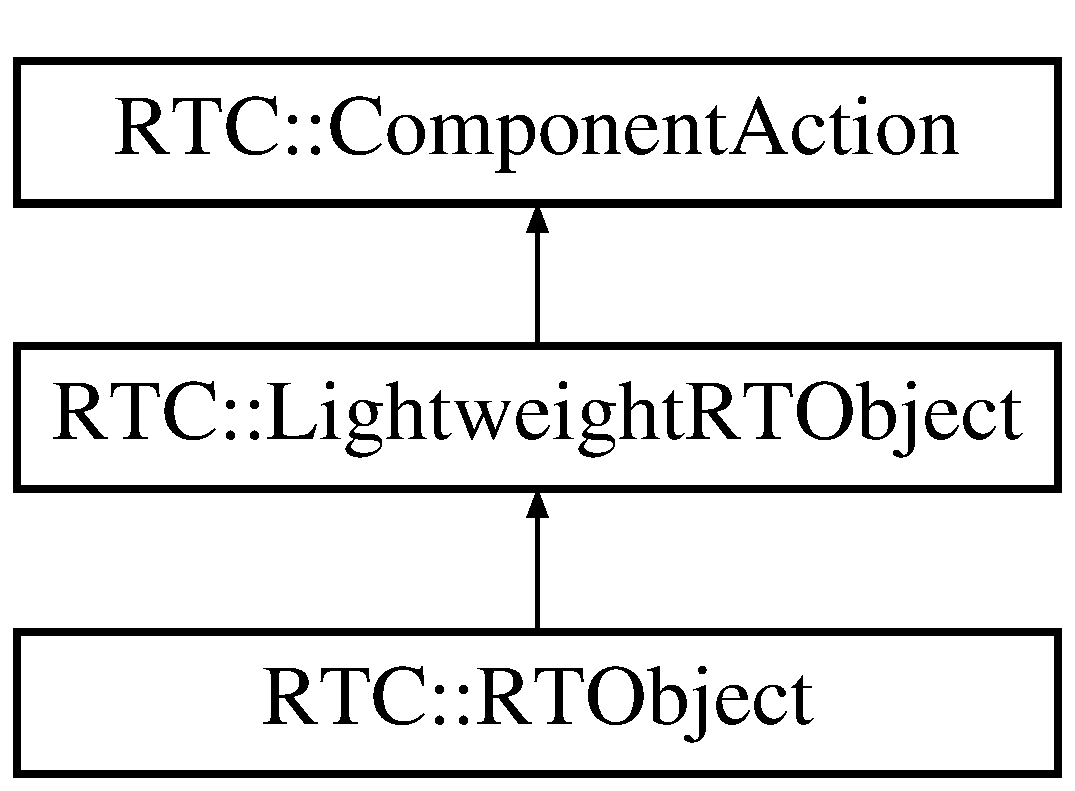
\includegraphics[height=3cm]{interfaceRTC_1_1ComponentAction}
\end{center}
\end{figure}
\subsection*{Public Member Functions}
\begin{CompactItemize}
\item 
{\bf Unique\-Id} {\bf attach\_\-executioncontext} (in {\bf Execution\-Context} exec\_\-context)
\item 
{\bf Return\-Code\_\-t} {\bf detach\_\-executioncontext} (in {\bf Unique\-Id} ec\_\-id)
\item 
{\bf Return\-Code\_\-t} {\bf on\_\-initialize} ()
\item 
{\bf Return\-Code\_\-t} {\bf on\_\-finalize} ()
\item 
{\bf Return\-Code\_\-t} {\bf on\_\-startup} (in {\bf Unique\-Id} ec\_\-id)
\item 
{\bf Return\-Code\_\-t} {\bf on\_\-shutdown} (in {\bf Unique\-Id} ec\_\-id)
\item 
{\bf Return\-Code\_\-t} {\bf on\_\-activated} (in {\bf Unique\-Id} ec\_\-id)
\item 
{\bf Return\-Code\_\-t} {\bf on\_\-deactivated} (in {\bf Unique\-Id} ec\_\-id)
\item 
{\bf Return\-Code\_\-t} {\bf on\_\-aborting} (in {\bf Unique\-Id} ec\_\-id)
\item 
{\bf Return\-Code\_\-t} {\bf on\_\-error} (in {\bf Unique\-Id} ec\_\-id)
\item 
{\bf Return\-Code\_\-t} {\bf on\_\-reset} (in {\bf Unique\-Id} ec\_\-id)
\end{CompactItemize}


\subsection{Detailed Description}
Lightweight\-RTC::Conponent\-Action interface. 



\subsection{Member Function Documentation}
\index{RTC::ComponentAction@{RTC::Component\-Action}!attach_executioncontext@{attach\_\-executioncontext}}
\index{attach_executioncontext@{attach\_\-executioncontext}!RTC::ComponentAction@{RTC::Component\-Action}}
\subsubsection{\setlength{\rightskip}{0pt plus 5cm}{\bf Unique\-Id} RTC::Component\-Action::attach\_\-executioncontext (in {\bf Execution\-Context} {\em exec\_\-context})}\label{interfaceRTC_1_1ComponentAction_RTC_1_1RTObjecta9}


\index{RTC::ComponentAction@{RTC::Component\-Action}!detach_executioncontext@{detach\_\-executioncontext}}
\index{detach_executioncontext@{detach\_\-executioncontext}!RTC::ComponentAction@{RTC::Component\-Action}}
\subsubsection{\setlength{\rightskip}{0pt plus 5cm}{\bf Return\-Code\_\-t} RTC::Component\-Action::detach\_\-executioncontext (in {\bf Unique\-Id} {\em ec\_\-id})}\label{interfaceRTC_1_1ComponentAction_RTC_1_1RTObjecta10}


\index{RTC::ComponentAction@{RTC::Component\-Action}!on_aborting@{on\_\-aborting}}
\index{on_aborting@{on\_\-aborting}!RTC::ComponentAction@{RTC::Component\-Action}}
\subsubsection{\setlength{\rightskip}{0pt plus 5cm}{\bf Return\-Code\_\-t} RTC::Component\-Action::on\_\-aborting (in {\bf Unique\-Id} {\em ec\_\-id})}\label{interfaceRTC_1_1ComponentAction_RTC_1_1RTObjecta17}


\index{RTC::ComponentAction@{RTC::Component\-Action}!on_activated@{on\_\-activated}}
\index{on_activated@{on\_\-activated}!RTC::ComponentAction@{RTC::Component\-Action}}
\subsubsection{\setlength{\rightskip}{0pt plus 5cm}{\bf Return\-Code\_\-t} RTC::Component\-Action::on\_\-activated (in {\bf Unique\-Id} {\em ec\_\-id})}\label{interfaceRTC_1_1ComponentAction_RTC_1_1RTObjecta15}


\index{RTC::ComponentAction@{RTC::Component\-Action}!on_deactivated@{on\_\-deactivated}}
\index{on_deactivated@{on\_\-deactivated}!RTC::ComponentAction@{RTC::Component\-Action}}
\subsubsection{\setlength{\rightskip}{0pt plus 5cm}{\bf Return\-Code\_\-t} RTC::Component\-Action::on\_\-deactivated (in {\bf Unique\-Id} {\em ec\_\-id})}\label{interfaceRTC_1_1ComponentAction_RTC_1_1RTObjecta16}


\index{RTC::ComponentAction@{RTC::Component\-Action}!on_error@{on\_\-error}}
\index{on_error@{on\_\-error}!RTC::ComponentAction@{RTC::Component\-Action}}
\subsubsection{\setlength{\rightskip}{0pt plus 5cm}{\bf Return\-Code\_\-t} RTC::Component\-Action::on\_\-error (in {\bf Unique\-Id} {\em ec\_\-id})}\label{interfaceRTC_1_1ComponentAction_RTC_1_1RTObjecta18}


\index{RTC::ComponentAction@{RTC::Component\-Action}!on_finalize@{on\_\-finalize}}
\index{on_finalize@{on\_\-finalize}!RTC::ComponentAction@{RTC::Component\-Action}}
\subsubsection{\setlength{\rightskip}{0pt plus 5cm}{\bf Return\-Code\_\-t} RTC::Component\-Action::on\_\-finalize ()}\label{interfaceRTC_1_1ComponentAction_RTC_1_1RTObjecta12}


\index{RTC::ComponentAction@{RTC::Component\-Action}!on_initialize@{on\_\-initialize}}
\index{on_initialize@{on\_\-initialize}!RTC::ComponentAction@{RTC::Component\-Action}}
\subsubsection{\setlength{\rightskip}{0pt plus 5cm}{\bf Return\-Code\_\-t} RTC::Component\-Action::on\_\-initialize ()}\label{interfaceRTC_1_1ComponentAction_RTC_1_1RTObjecta11}


\index{RTC::ComponentAction@{RTC::Component\-Action}!on_reset@{on\_\-reset}}
\index{on_reset@{on\_\-reset}!RTC::ComponentAction@{RTC::Component\-Action}}
\subsubsection{\setlength{\rightskip}{0pt plus 5cm}{\bf Return\-Code\_\-t} RTC::Component\-Action::on\_\-reset (in {\bf Unique\-Id} {\em ec\_\-id})}\label{interfaceRTC_1_1ComponentAction_RTC_1_1RTObjecta19}


\index{RTC::ComponentAction@{RTC::Component\-Action}!on_shutdown@{on\_\-shutdown}}
\index{on_shutdown@{on\_\-shutdown}!RTC::ComponentAction@{RTC::Component\-Action}}
\subsubsection{\setlength{\rightskip}{0pt plus 5cm}{\bf Return\-Code\_\-t} RTC::Component\-Action::on\_\-shutdown (in {\bf Unique\-Id} {\em ec\_\-id})}\label{interfaceRTC_1_1ComponentAction_RTC_1_1RTObjecta14}


\index{RTC::ComponentAction@{RTC::Component\-Action}!on_startup@{on\_\-startup}}
\index{on_startup@{on\_\-startup}!RTC::ComponentAction@{RTC::Component\-Action}}
\subsubsection{\setlength{\rightskip}{0pt plus 5cm}{\bf Return\-Code\_\-t} RTC::Component\-Action::on\_\-startup (in {\bf Unique\-Id} {\em ec\_\-id})}\label{interfaceRTC_1_1ComponentAction_RTC_1_1RTObjecta13}




The documentation for this interface was generated from the following file:\begin{CompactItemize}
\item 
{\bf RTC.idl}\end{CompactItemize}

\section{��¤�� RTC::Component\-Profile}
\label{structRTC_1_1ComponentProfile}\index{RTC::ComponentProfile@{RTC::ComponentProfile}}
Introspection::Component\-Profile structure.  


{\tt import \char`\"{}RTC.idl\char`\"{};}

\subsection*{Public �ѿ�}
\begin{CompactItemize}
\item 
string {\bf instance\_\-name}
\item 
string {\bf type\_\-name}
\item 
string {\bf description}
\item 
string {\bf version}
\item 
string {\bf vendor}
\item 
string {\bf category}
\item 
{\bf Port\-Profile\-List} {\bf port\_\-profiles}
\item 
{\bf RTObject} {\bf parent}
\item 
{\bf NVList} {\bf properties}
\end{CompactItemize}


\subsection{����}
Introspection::Component\-Profile structure. 



\subsection{�ѿ�}
\index{RTC::ComponentProfile@{RTC::Component\-Profile}!category@{category}}
\index{category@{category}!RTC::ComponentProfile@{RTC::Component\-Profile}}
\subsubsection{\setlength{\rightskip}{0pt plus 5cm}string {\bf RTC::Component\-Profile::category}}\label{structRTC_1_1ComponentProfile_RTC_1_1ComponentProfileo5}


\index{RTC::ComponentProfile@{RTC::Component\-Profile}!description@{description}}
\index{description@{description}!RTC::ComponentProfile@{RTC::Component\-Profile}}
\subsubsection{\setlength{\rightskip}{0pt plus 5cm}string {\bf RTC::Component\-Profile::description}}\label{structRTC_1_1ComponentProfile_RTC_1_1ComponentProfileo2}


\index{RTC::ComponentProfile@{RTC::Component\-Profile}!instance_name@{instance\_\-name}}
\index{instance_name@{instance\_\-name}!RTC::ComponentProfile@{RTC::Component\-Profile}}
\subsubsection{\setlength{\rightskip}{0pt plus 5cm}string {\bf RTC::Component\-Profile::instance\_\-name}}\label{structRTC_1_1ComponentProfile_RTC_1_1ComponentProfileo0}


\index{RTC::ComponentProfile@{RTC::Component\-Profile}!parent@{parent}}
\index{parent@{parent}!RTC::ComponentProfile@{RTC::Component\-Profile}}
\subsubsection{\setlength{\rightskip}{0pt plus 5cm}{\bf RTObject} {\bf RTC::Component\-Profile::parent}}\label{structRTC_1_1ComponentProfile_RTC_1_1ComponentProfileo7}


\index{RTC::ComponentProfile@{RTC::Component\-Profile}!port_profiles@{port\_\-profiles}}
\index{port_profiles@{port\_\-profiles}!RTC::ComponentProfile@{RTC::Component\-Profile}}
\subsubsection{\setlength{\rightskip}{0pt plus 5cm}{\bf Port\-Profile\-List} {\bf RTC::Component\-Profile::port\_\-profiles}}\label{structRTC_1_1ComponentProfile_RTC_1_1ComponentProfileo6}


\index{RTC::ComponentProfile@{RTC::Component\-Profile}!properties@{properties}}
\index{properties@{properties}!RTC::ComponentProfile@{RTC::Component\-Profile}}
\subsubsection{\setlength{\rightskip}{0pt plus 5cm}{\bf NVList} {\bf RTC::Component\-Profile::properties}}\label{structRTC_1_1ComponentProfile_RTC_1_1ComponentProfileo8}


\index{RTC::ComponentProfile@{RTC::Component\-Profile}!type_name@{type\_\-name}}
\index{type_name@{type\_\-name}!RTC::ComponentProfile@{RTC::Component\-Profile}}
\subsubsection{\setlength{\rightskip}{0pt plus 5cm}string {\bf RTC::Component\-Profile::type\_\-name}}\label{structRTC_1_1ComponentProfile_RTC_1_1ComponentProfileo1}


\index{RTC::ComponentProfile@{RTC::Component\-Profile}!vendor@{vendor}}
\index{vendor@{vendor}!RTC::ComponentProfile@{RTC::Component\-Profile}}
\subsubsection{\setlength{\rightskip}{0pt plus 5cm}string {\bf RTC::Component\-Profile::vendor}}\label{structRTC_1_1ComponentProfile_RTC_1_1ComponentProfileo4}


\index{RTC::ComponentProfile@{RTC::Component\-Profile}!version@{version}}
\index{version@{version}!RTC::ComponentProfile@{RTC::Component\-Profile}}
\subsubsection{\setlength{\rightskip}{0pt plus 5cm}string {\bf RTC::Component\-Profile::version}}\label{structRTC_1_1ComponentProfile_RTC_1_1ComponentProfileo3}




���ι�¤�Τ������ϼ��Υե����뤫����������ޤ���:\begin{CompactItemize}
\item 
{\bf RTC.idl}\end{CompactItemize}

\section{���󥿥ե����� SDOPackage::Configuration}
\label{interfaceSDOPackage_1_1Configuration}\index{SDOPackage::Configuration@{SDOPackage::Configuration}}
{\tt import \char`\"{}SDOPackage.idl\char`\"{};}

\subsection*{Public �᥽�å�}
\begin{CompactItemize}
\item 
boolean {\bf set\_\-device\_\-profile} (in {\bf Device\-Profile} d\-Profile)  raises (Invalid\-Parameter, Not\-Available, Internal\-Error)
\item 
boolean {\bf set\_\-service\_\-profile} (in {\bf Service\-Profile} s\-Profile)  raises (Invalid\-Parameter, Not\-Available, Internal\-Error)
\item 
boolean {\bf add\_\-organization} (in {\bf Organization} org)  raises (Invalid\-Parameter, Not\-Available, Internal\-Error)
\item 
boolean {\bf remove\_\-service\_\-profile} (in {\bf Unique\-Identifier} id)  raises (Invalid\-Parameter, Not\-Available, Internal\-Error)
\item 
boolean {\bf remove\_\-organization} (in {\bf Unique\-Identifier} organization\_\-id)  raises (Invalid\-Parameter, Not\-Available, Internal\-Error)
\item 
{\bf Parameter\-List} {\bf get\_\-configuration\_\-parameters} ()  raises (Not\-Available, Internal\-Error)
\item 
{\bf NVList} {\bf get\_\-configuration\_\-parameter\_\-values} ()  raises (Not\-Available, Internal\-Error)
\item 
any {\bf get\_\-configuration\_\-parameter\_\-value} (in string name)  raises (Invalid\-Parameter, Not\-Available, Internal\-Error)
\item 
boolean {\bf set\_\-configuration\_\-parameter} (in string name, in any value)  raises (Invalid\-Parameter, Not\-Available, Internal\-Error)
\item 
{\bf Configuration\-Set\-List} {\bf get\_\-configuration\_\-sets} ()  raises (Not\-Available, Internal\-Error)
\item 
{\bf Configuration\-Set} {\bf get\_\-configuration\_\-set} (in {\bf Unique\-Identifier} config\_\-id)  raises (Not\-Available, Internal\-Error)
\item 
boolean {\bf set\_\-configuration\_\-set\_\-values} (in {\bf Unique\-Identifier} config\_\-id, in {\bf Configuration\-Set} configuration\_\-set)  raises (Invalid\-Parameter, Not\-Available, Internal\-Error)
\item 
{\bf Configuration\-Set} {\bf get\_\-active\_\-configuration\_\-set} ()  raises (Not\-Available, Internal\-Error)
\item 
boolean {\bf add\_\-configuration\_\-set} (in {\bf Configuration\-Set} configuration\_\-set)  raises (Invalid\-Parameter, Not\-Available, Internal\-Error)
\item 
boolean {\bf remove\_\-configuration\_\-set} (in {\bf Unique\-Identifier} config\_\-id)  raises (Invalid\-Parameter, Not\-Available, Internal\-Error)
\item 
boolean {\bf activate\_\-configuration\_\-set} (in {\bf Unique\-Identifier} config\_\-id)  raises (Invalid\-Parameter, Not\-Available, Internal\-Error)
\end{CompactItemize}


\subsection{�ؿ�}
\index{SDOPackage::Configuration@{SDOPackage::Configuration}!activate_configuration_set@{activate\_\-configuration\_\-set}}
\index{activate_configuration_set@{activate\_\-configuration\_\-set}!SDOPackage::Configuration@{SDOPackage::Configuration}}
\subsubsection{\setlength{\rightskip}{0pt plus 5cm}boolean SDOPackage::Configuration::activate\_\-configuration\_\-set (in {\bf Unique\-Identifier} {\em config\_\-id})  raises (Invalid\-Parameter, Not\-Available, Internal\-Error)}\label{interfaceSDOPackage_1_1Configuration_SDOPackage_1_1Configurationa15}


\index{SDOPackage::Configuration@{SDOPackage::Configuration}!add_configuration_set@{add\_\-configuration\_\-set}}
\index{add_configuration_set@{add\_\-configuration\_\-set}!SDOPackage::Configuration@{SDOPackage::Configuration}}
\subsubsection{\setlength{\rightskip}{0pt plus 5cm}boolean SDOPackage::Configuration::add\_\-configuration\_\-set (in {\bf Configuration\-Set} {\em configuration\_\-set})  raises (Invalid\-Parameter, Not\-Available, Internal\-Error)}\label{interfaceSDOPackage_1_1Configuration_SDOPackage_1_1Configurationa13}


\index{SDOPackage::Configuration@{SDOPackage::Configuration}!add_organization@{add\_\-organization}}
\index{add_organization@{add\_\-organization}!SDOPackage::Configuration@{SDOPackage::Configuration}}
\subsubsection{\setlength{\rightskip}{0pt plus 5cm}boolean SDOPackage::Configuration::add\_\-organization (in {\bf Organization} {\em org})  raises (Invalid\-Parameter, Not\-Available, Internal\-Error)}\label{interfaceSDOPackage_1_1Configuration_SDOPackage_1_1Configurationa2}


\index{SDOPackage::Configuration@{SDOPackage::Configuration}!get_active_configuration_set@{get\_\-active\_\-configuration\_\-set}}
\index{get_active_configuration_set@{get\_\-active\_\-configuration\_\-set}!SDOPackage::Configuration@{SDOPackage::Configuration}}
\subsubsection{\setlength{\rightskip}{0pt plus 5cm}{\bf Configuration\-Set} SDOPackage::Configuration::get\_\-active\_\-configuration\_\-set ()  raises (Not\-Available, Internal\-Error)}\label{interfaceSDOPackage_1_1Configuration_SDOPackage_1_1Configurationa12}


\index{SDOPackage::Configuration@{SDOPackage::Configuration}!get_configuration_parameter_value@{get\_\-configuration\_\-parameter\_\-value}}
\index{get_configuration_parameter_value@{get\_\-configuration\_\-parameter\_\-value}!SDOPackage::Configuration@{SDOPackage::Configuration}}
\subsubsection{\setlength{\rightskip}{0pt plus 5cm}any SDOPackage::Configuration::get\_\-configuration\_\-parameter\_\-value (in string {\em name})  raises (Invalid\-Parameter, Not\-Available, Internal\-Error)}\label{interfaceSDOPackage_1_1Configuration_SDOPackage_1_1Configurationa7}


\index{SDOPackage::Configuration@{SDOPackage::Configuration}!get_configuration_parameter_values@{get\_\-configuration\_\-parameter\_\-values}}
\index{get_configuration_parameter_values@{get\_\-configuration\_\-parameter\_\-values}!SDOPackage::Configuration@{SDOPackage::Configuration}}
\subsubsection{\setlength{\rightskip}{0pt plus 5cm}{\bf NVList} SDOPackage::Configuration::get\_\-configuration\_\-parameter\_\-values ()  raises (Not\-Available, Internal\-Error)}\label{interfaceSDOPackage_1_1Configuration_SDOPackage_1_1Configurationa6}


\index{SDOPackage::Configuration@{SDOPackage::Configuration}!get_configuration_parameters@{get\_\-configuration\_\-parameters}}
\index{get_configuration_parameters@{get\_\-configuration\_\-parameters}!SDOPackage::Configuration@{SDOPackage::Configuration}}
\subsubsection{\setlength{\rightskip}{0pt plus 5cm}{\bf Parameter\-List} SDOPackage::Configuration::get\_\-configuration\_\-parameters ()  raises (Not\-Available, Internal\-Error)}\label{interfaceSDOPackage_1_1Configuration_SDOPackage_1_1Configurationa5}


\index{SDOPackage::Configuration@{SDOPackage::Configuration}!get_configuration_set@{get\_\-configuration\_\-set}}
\index{get_configuration_set@{get\_\-configuration\_\-set}!SDOPackage::Configuration@{SDOPackage::Configuration}}
\subsubsection{\setlength{\rightskip}{0pt plus 5cm}{\bf Configuration\-Set} SDOPackage::Configuration::get\_\-configuration\_\-set (in {\bf Unique\-Identifier} {\em config\_\-id})  raises (Not\-Available, Internal\-Error)}\label{interfaceSDOPackage_1_1Configuration_SDOPackage_1_1Configurationa10}


\index{SDOPackage::Configuration@{SDOPackage::Configuration}!get_configuration_sets@{get\_\-configuration\_\-sets}}
\index{get_configuration_sets@{get\_\-configuration\_\-sets}!SDOPackage::Configuration@{SDOPackage::Configuration}}
\subsubsection{\setlength{\rightskip}{0pt plus 5cm}{\bf Configuration\-Set\-List} SDOPackage::Configuration::get\_\-configuration\_\-sets ()  raises (Not\-Available, Internal\-Error)}\label{interfaceSDOPackage_1_1Configuration_SDOPackage_1_1Configurationa9}


\index{SDOPackage::Configuration@{SDOPackage::Configuration}!remove_configuration_set@{remove\_\-configuration\_\-set}}
\index{remove_configuration_set@{remove\_\-configuration\_\-set}!SDOPackage::Configuration@{SDOPackage::Configuration}}
\subsubsection{\setlength{\rightskip}{0pt plus 5cm}boolean SDOPackage::Configuration::remove\_\-configuration\_\-set (in {\bf Unique\-Identifier} {\em config\_\-id})  raises (Invalid\-Parameter, Not\-Available, Internal\-Error)}\label{interfaceSDOPackage_1_1Configuration_SDOPackage_1_1Configurationa14}


\index{SDOPackage::Configuration@{SDOPackage::Configuration}!remove_organization@{remove\_\-organization}}
\index{remove_organization@{remove\_\-organization}!SDOPackage::Configuration@{SDOPackage::Configuration}}
\subsubsection{\setlength{\rightskip}{0pt plus 5cm}boolean SDOPackage::Configuration::remove\_\-organization (in {\bf Unique\-Identifier} {\em organization\_\-id})  raises (Invalid\-Parameter, Not\-Available, Internal\-Error)}\label{interfaceSDOPackage_1_1Configuration_SDOPackage_1_1Configurationa4}


\index{SDOPackage::Configuration@{SDOPackage::Configuration}!remove_service_profile@{remove\_\-service\_\-profile}}
\index{remove_service_profile@{remove\_\-service\_\-profile}!SDOPackage::Configuration@{SDOPackage::Configuration}}
\subsubsection{\setlength{\rightskip}{0pt plus 5cm}boolean SDOPackage::Configuration::remove\_\-service\_\-profile (in {\bf Unique\-Identifier} {\em id})  raises (Invalid\-Parameter, Not\-Available, Internal\-Error)}\label{interfaceSDOPackage_1_1Configuration_SDOPackage_1_1Configurationa3}


\index{SDOPackage::Configuration@{SDOPackage::Configuration}!set_configuration_parameter@{set\_\-configuration\_\-parameter}}
\index{set_configuration_parameter@{set\_\-configuration\_\-parameter}!SDOPackage::Configuration@{SDOPackage::Configuration}}
\subsubsection{\setlength{\rightskip}{0pt plus 5cm}boolean SDOPackage::Configuration::set\_\-configuration\_\-parameter (in string {\em name}, in any {\em value})  raises (Invalid\-Parameter, Not\-Available, Internal\-Error)}\label{interfaceSDOPackage_1_1Configuration_SDOPackage_1_1Configurationa8}


\index{SDOPackage::Configuration@{SDOPackage::Configuration}!set_configuration_set_values@{set\_\-configuration\_\-set\_\-values}}
\index{set_configuration_set_values@{set\_\-configuration\_\-set\_\-values}!SDOPackage::Configuration@{SDOPackage::Configuration}}
\subsubsection{\setlength{\rightskip}{0pt plus 5cm}boolean SDOPackage::Configuration::set\_\-configuration\_\-set\_\-values (in {\bf Unique\-Identifier} {\em config\_\-id}, in {\bf Configuration\-Set} {\em configuration\_\-set})  raises (Invalid\-Parameter, Not\-Available, Internal\-Error)}\label{interfaceSDOPackage_1_1Configuration_SDOPackage_1_1Configurationa11}


\index{SDOPackage::Configuration@{SDOPackage::Configuration}!set_device_profile@{set\_\-device\_\-profile}}
\index{set_device_profile@{set\_\-device\_\-profile}!SDOPackage::Configuration@{SDOPackage::Configuration}}
\subsubsection{\setlength{\rightskip}{0pt plus 5cm}boolean SDOPackage::Configuration::set\_\-device\_\-profile (in {\bf Device\-Profile} {\em d\-Profile})  raises (Invalid\-Parameter, Not\-Available, Internal\-Error)}\label{interfaceSDOPackage_1_1Configuration_SDOPackage_1_1Configurationa0}


\index{SDOPackage::Configuration@{SDOPackage::Configuration}!set_service_profile@{set\_\-service\_\-profile}}
\index{set_service_profile@{set\_\-service\_\-profile}!SDOPackage::Configuration@{SDOPackage::Configuration}}
\subsubsection{\setlength{\rightskip}{0pt plus 5cm}boolean SDOPackage::Configuration::set\_\-service\_\-profile (in {\bf Service\-Profile} {\em s\-Profile})  raises (Invalid\-Parameter, Not\-Available, Internal\-Error)}\label{interfaceSDOPackage_1_1Configuration_SDOPackage_1_1Configurationa1}




���Υ��󥿥ե������������ϼ��Υե����뤫����������ޤ���:\begin{CompactItemize}
\item 
{\bf SDOPackage.idl}\end{CompactItemize}

\section{SDOPackage::Configuration\-Set Struct Reference}
\label{structSDOPackage_1_1ConfigurationSet}\index{SDOPackage::ConfigurationSet@{SDOPackage::ConfigurationSet}}
{\tt import \char`\"{}SDOPackage.idl\char`\"{};}

\subsection*{Public Attributes}
\begin{CompactItemize}
\item 
string {\bf id}
\item 
string {\bf description}
\item 
{\bf NVList} {\bf configuration\_\-data}
\end{CompactItemize}


\subsection{Member Data Documentation}
\index{SDOPackage::ConfigurationSet@{SDOPackage::Configuration\-Set}!configuration_data@{configuration\_\-data}}
\index{configuration_data@{configuration\_\-data}!SDOPackage::ConfigurationSet@{SDOPackage::Configuration\-Set}}
\subsubsection{\setlength{\rightskip}{0pt plus 5cm}{\bf NVList} {\bf SDOPackage::Configuration\-Set::configuration\_\-data}}\label{structSDOPackage_1_1ConfigurationSet_SDOPackage_1_1ConfigurationSeto2}


\index{SDOPackage::ConfigurationSet@{SDOPackage::Configuration\-Set}!description@{description}}
\index{description@{description}!SDOPackage::ConfigurationSet@{SDOPackage::Configuration\-Set}}
\subsubsection{\setlength{\rightskip}{0pt plus 5cm}string {\bf SDOPackage::Configuration\-Set::description}}\label{structSDOPackage_1_1ConfigurationSet_SDOPackage_1_1ConfigurationSeto1}


\index{SDOPackage::ConfigurationSet@{SDOPackage::Configuration\-Set}!id@{id}}
\index{id@{id}!SDOPackage::ConfigurationSet@{SDOPackage::Configuration\-Set}}
\subsubsection{\setlength{\rightskip}{0pt plus 5cm}string {\bf SDOPackage::Configuration\-Set::id}}\label{structSDOPackage_1_1ConfigurationSet_SDOPackage_1_1ConfigurationSeto0}




The documentation for this struct was generated from the following file:\begin{CompactItemize}
\item 
{\bf SDOPackage.idl}\end{CompactItemize}

\section{��¤�� RTC::Connector\-Profile}
\label{structRTC_1_1ConnectorProfile}\index{RTC::ConnectorProfile@{RTC::ConnectorProfile}}
Introspection::Connector\-Profile structure.  


{\tt import \char`\"{}RTC.idl\char`\"{};}

\subsection*{Public �ѿ�}
\begin{CompactItemize}
\item 
string {\bf name}
\item 
{\bf Unique\-Identifier} {\bf connector\_\-id}
\item 
{\bf Port\-List} {\bf ports}
\item 
{\bf NVList} {\bf properties}
\end{CompactItemize}


\subsection{����}
Introspection::Connector\-Profile structure. 



\subsection{�ѿ�}
\index{RTC::ConnectorProfile@{RTC::Connector\-Profile}!connector_id@{connector\_\-id}}
\index{connector_id@{connector\_\-id}!RTC::ConnectorProfile@{RTC::Connector\-Profile}}
\subsubsection{\setlength{\rightskip}{0pt plus 5cm}{\bf Unique\-Identifier} {\bf RTC::Connector\-Profile::connector\_\-id}}\label{structRTC_1_1ConnectorProfile_RTC_1_1ConnectorProfileo1}


\index{RTC::ConnectorProfile@{RTC::Connector\-Profile}!name@{name}}
\index{name@{name}!RTC::ConnectorProfile@{RTC::Connector\-Profile}}
\subsubsection{\setlength{\rightskip}{0pt plus 5cm}string {\bf RTC::Connector\-Profile::name}}\label{structRTC_1_1ConnectorProfile_RTC_1_1ConnectorProfileo0}


\index{RTC::ConnectorProfile@{RTC::Connector\-Profile}!ports@{ports}}
\index{ports@{ports}!RTC::ConnectorProfile@{RTC::Connector\-Profile}}
\subsubsection{\setlength{\rightskip}{0pt plus 5cm}{\bf Port\-List} {\bf RTC::Connector\-Profile::ports}}\label{structRTC_1_1ConnectorProfile_RTC_1_1ConnectorProfileo2}


\index{RTC::ConnectorProfile@{RTC::Connector\-Profile}!properties@{properties}}
\index{properties@{properties}!RTC::ConnectorProfile@{RTC::Connector\-Profile}}
\subsubsection{\setlength{\rightskip}{0pt plus 5cm}{\bf NVList} {\bf RTC::Connector\-Profile::properties}}\label{structRTC_1_1ConnectorProfile_RTC_1_1ConnectorProfileo3}




���ι�¤�Τ������ϼ��Υե����뤫����������ޤ���:\begin{CompactItemize}
\item 
{\bf RTC.idl}\end{CompactItemize}

\section{RTC::Data\-Flow\-Component\-Action Interface Reference}
\label{interfaceRTC_1_1DataFlowComponentAction}\index{RTC::DataFlowComponentAction@{RTC::DataFlowComponentAction}}
Execution\-Semantics::Data\-Flow\-Component\-Action interface.  


{\tt import \char`\"{}RTC.idl\char`\"{};}

Inheritance diagram for RTC::Data\-Flow\-Component\-Action::\begin{figure}[H]
\begin{center}
\leavevmode
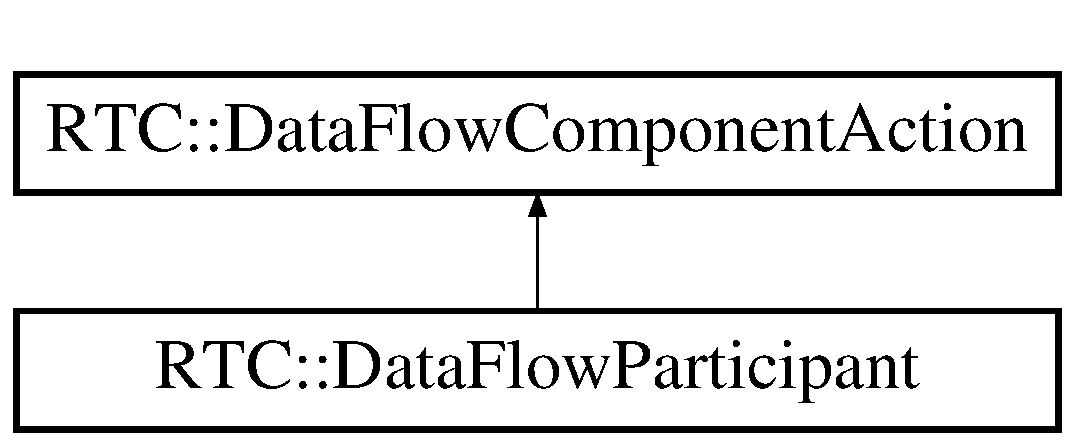
\includegraphics[height=2cm]{interfaceRTC_1_1DataFlowComponentAction}
\end{center}
\end{figure}
\subsection*{Public Member Functions}
\begin{CompactItemize}
\item 
{\bf Return\-Code\_\-t} {\bf on\_\-execute} (in {\bf Unique\-Id} ec\_\-id)
\item 
{\bf Return\-Code\_\-t} {\bf on\_\-state\_\-update} (in {\bf Unique\-Id} ec\_\-id)
\item 
{\bf Return\-Code\_\-t} {\bf on\_\-rate\_\-changed} (in {\bf Unique\-Id} ec\_\-id)
\end{CompactItemize}


\subsection{Detailed Description}
Execution\-Semantics::Data\-Flow\-Component\-Action interface. 

----------------------------------------------------------- Execution\-Semantics Package ------------------------------------------------------------/

/$\ast$! 



\subsection{Member Function Documentation}
\index{RTC::DataFlowComponentAction@{RTC::Data\-Flow\-Component\-Action}!on_execute@{on\_\-execute}}
\index{on_execute@{on\_\-execute}!RTC::DataFlowComponentAction@{RTC::Data\-Flow\-Component\-Action}}
\subsubsection{\setlength{\rightskip}{0pt plus 5cm}{\bf Return\-Code\_\-t} RTC::Data\-Flow\-Component\-Action::on\_\-execute (in {\bf Unique\-Id} {\em ec\_\-id})}\label{interfaceRTC_1_1DataFlowComponentAction_RTC_1_1DataFlowParticipanta0}


\index{RTC::DataFlowComponentAction@{RTC::Data\-Flow\-Component\-Action}!on_rate_changed@{on\_\-rate\_\-changed}}
\index{on_rate_changed@{on\_\-rate\_\-changed}!RTC::DataFlowComponentAction@{RTC::Data\-Flow\-Component\-Action}}
\subsubsection{\setlength{\rightskip}{0pt plus 5cm}{\bf Return\-Code\_\-t} RTC::Data\-Flow\-Component\-Action::on\_\-rate\_\-changed (in {\bf Unique\-Id} {\em ec\_\-id})}\label{interfaceRTC_1_1DataFlowComponentAction_RTC_1_1DataFlowParticipanta2}


\index{RTC::DataFlowComponentAction@{RTC::Data\-Flow\-Component\-Action}!on_state_update@{on\_\-state\_\-update}}
\index{on_state_update@{on\_\-state\_\-update}!RTC::DataFlowComponentAction@{RTC::Data\-Flow\-Component\-Action}}
\subsubsection{\setlength{\rightskip}{0pt plus 5cm}{\bf Return\-Code\_\-t} RTC::Data\-Flow\-Component\-Action::on\_\-state\_\-update (in {\bf Unique\-Id} {\em ec\_\-id})}\label{interfaceRTC_1_1DataFlowComponentAction_RTC_1_1DataFlowParticipanta1}




The documentation for this interface was generated from the following file:\begin{CompactItemize}
\item 
{\bf RTC.idl}\end{CompactItemize}

\section{���󥿥ե����� RTC::Data\-Flow\-Participant}
\label{interfaceRTC_1_1DataFlowParticipant}\index{RTC::DataFlowParticipant@{RTC::DataFlowParticipant}}
Execution\-Semantics::Data\-Flow\-Participant component.  


{\tt import \char`\"{}RTC.idl\char`\"{};}

RTC::Data\-Flow\-Participant���Ф���Ѿ������:\begin{figure}[H]
\begin{center}
\leavevmode
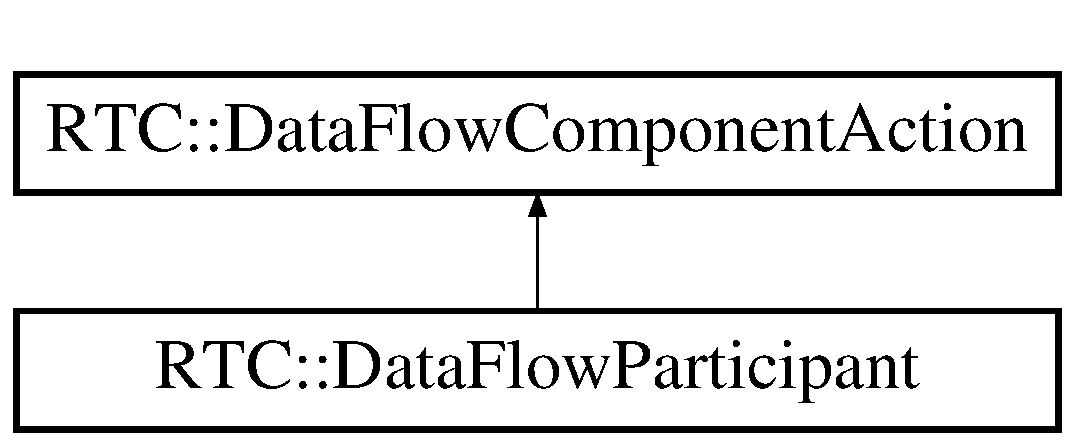
\includegraphics[height=2cm]{interfaceRTC_1_1DataFlowParticipant}
\end{center}
\end{figure}
\subsection*{Public �᥽�å�}
\begin{CompactItemize}
\item 
{\bf Return\-Code\_\-t} {\bf on\_\-execute} (in {\bf Unique\-Id} ec\_\-id)
\item 
{\bf Return\-Code\_\-t} {\bf on\_\-state\_\-update} (in {\bf Unique\-Id} ec\_\-id)
\item 
{\bf Return\-Code\_\-t} {\bf on\_\-rate\_\-changed} (in {\bf Unique\-Id} ec\_\-id)
\end{CompactItemize}


\subsection{����}
Execution\-Semantics::Data\-Flow\-Participant component. 



\subsection{�ؿ�}
\index{RTC::DataFlowParticipant@{RTC::Data\-Flow\-Participant}!on_execute@{on\_\-execute}}
\index{on_execute@{on\_\-execute}!RTC::DataFlowParticipant@{RTC::Data\-Flow\-Participant}}
\subsubsection{\setlength{\rightskip}{0pt plus 5cm}{\bf Return\-Code\_\-t} RTC::Data\-Flow\-Component\-Action::on\_\-execute (in {\bf Unique\-Id} {\em ec\_\-id})\hspace{0.3cm}{\tt  [inherited]}}\label{interfaceRTC_1_1DataFlowComponentAction_RTC_1_1DataFlowParticipanta0}


\index{RTC::DataFlowParticipant@{RTC::Data\-Flow\-Participant}!on_rate_changed@{on\_\-rate\_\-changed}}
\index{on_rate_changed@{on\_\-rate\_\-changed}!RTC::DataFlowParticipant@{RTC::Data\-Flow\-Participant}}
\subsubsection{\setlength{\rightskip}{0pt plus 5cm}{\bf Return\-Code\_\-t} RTC::Data\-Flow\-Component\-Action::on\_\-rate\_\-changed (in {\bf Unique\-Id} {\em ec\_\-id})\hspace{0.3cm}{\tt  [inherited]}}\label{interfaceRTC_1_1DataFlowComponentAction_RTC_1_1DataFlowParticipanta2}


\index{RTC::DataFlowParticipant@{RTC::Data\-Flow\-Participant}!on_state_update@{on\_\-state\_\-update}}
\index{on_state_update@{on\_\-state\_\-update}!RTC::DataFlowParticipant@{RTC::Data\-Flow\-Participant}}
\subsubsection{\setlength{\rightskip}{0pt plus 5cm}{\bf Return\-Code\_\-t} RTC::Data\-Flow\-Component\-Action::on\_\-state\_\-update (in {\bf Unique\-Id} {\em ec\_\-id})\hspace{0.3cm}{\tt  [inherited]}}\label{interfaceRTC_1_1DataFlowComponentAction_RTC_1_1DataFlowParticipanta1}




���Υ��󥿥ե������������ϼ��Υե����뤫����������ޤ���:\begin{CompactItemize}
\item 
{\bf RTC.idl}\end{CompactItemize}

\section{SDOPackage::Device\-Profile Struct Reference}
\label{structSDOPackage_1_1DeviceProfile}\index{SDOPackage::DeviceProfile@{SDOPackage::DeviceProfile}}
{\tt import \char`\"{}SDOPackage.idl\char`\"{};}

\subsection*{Public Attributes}
\begin{CompactItemize}
\item 
string {\bf device\_\-type}
\item 
string {\bf manufacturer}
\item 
string {\bf model}
\item 
string {\bf version}
\item 
{\bf NVList} {\bf properties}
\end{CompactItemize}


\subsection{Member Data Documentation}
\index{SDOPackage::DeviceProfile@{SDOPackage::Device\-Profile}!device_type@{device\_\-type}}
\index{device_type@{device\_\-type}!SDOPackage::DeviceProfile@{SDOPackage::Device\-Profile}}
\subsubsection{\setlength{\rightskip}{0pt plus 5cm}string {\bf SDOPackage::Device\-Profile::device\_\-type}}\label{structSDOPackage_1_1DeviceProfile_SDOPackage_1_1DeviceProfileo0}


\index{SDOPackage::DeviceProfile@{SDOPackage::Device\-Profile}!manufacturer@{manufacturer}}
\index{manufacturer@{manufacturer}!SDOPackage::DeviceProfile@{SDOPackage::Device\-Profile}}
\subsubsection{\setlength{\rightskip}{0pt plus 5cm}string {\bf SDOPackage::Device\-Profile::manufacturer}}\label{structSDOPackage_1_1DeviceProfile_SDOPackage_1_1DeviceProfileo1}


\index{SDOPackage::DeviceProfile@{SDOPackage::Device\-Profile}!model@{model}}
\index{model@{model}!SDOPackage::DeviceProfile@{SDOPackage::Device\-Profile}}
\subsubsection{\setlength{\rightskip}{0pt plus 5cm}string {\bf SDOPackage::Device\-Profile::model}}\label{structSDOPackage_1_1DeviceProfile_SDOPackage_1_1DeviceProfileo2}


\index{SDOPackage::DeviceProfile@{SDOPackage::Device\-Profile}!properties@{properties}}
\index{properties@{properties}!SDOPackage::DeviceProfile@{SDOPackage::Device\-Profile}}
\subsubsection{\setlength{\rightskip}{0pt plus 5cm}{\bf NVList} {\bf SDOPackage::Device\-Profile::properties}}\label{structSDOPackage_1_1DeviceProfile_SDOPackage_1_1DeviceProfileo4}


\index{SDOPackage::DeviceProfile@{SDOPackage::Device\-Profile}!version@{version}}
\index{version@{version}!SDOPackage::DeviceProfile@{SDOPackage::Device\-Profile}}
\subsubsection{\setlength{\rightskip}{0pt plus 5cm}string {\bf SDOPackage::Device\-Profile::version}}\label{structSDOPackage_1_1DeviceProfile_SDOPackage_1_1DeviceProfileo3}




The documentation for this struct was generated from the following file:\begin{CompactItemize}
\item 
{\bf SDOPackage.idl}\end{CompactItemize}

\section{SDOPackage::Enumeration\-Type Struct Reference}
\label{structSDOPackage_1_1EnumerationType}\index{SDOPackage::EnumerationType@{SDOPackage::EnumerationType}}
{\tt import \char`\"{}SDOPackage.idl\char`\"{};}

\subsection*{Public Attributes}
\begin{CompactItemize}
\item 
{\bf String\-List} {\bf enumerated\_\-values}
\end{CompactItemize}


\subsection{Member Data Documentation}
\index{SDOPackage::EnumerationType@{SDOPackage::Enumeration\-Type}!enumerated_values@{enumerated\_\-values}}
\index{enumerated_values@{enumerated\_\-values}!SDOPackage::EnumerationType@{SDOPackage::Enumeration\-Type}}
\subsubsection{\setlength{\rightskip}{0pt plus 5cm}{\bf String\-List} {\bf SDOPackage::Enumeration\-Type::enumerated\_\-values}}\label{structSDOPackage_1_1EnumerationType_SDOPackage_1_1EnumerationTypeo0}




The documentation for this struct was generated from the following file:\begin{CompactItemize}
\item 
{\bf SDOPackage.idl}\end{CompactItemize}

\section{���󥿥ե����� RTC::Execution\-Context}
\label{interfaceRTC_1_1ExecutionContext}\index{RTC::ExecutionContext@{RTC::ExecutionContext}}
Lightweight\-RTC::Execution\-Context interface.  


{\tt import \char`\"{}RTC.idl\char`\"{};}

RTC::Execution\-Context���Ф���Ѿ������:\begin{figure}[H]
\begin{center}
\leavevmode
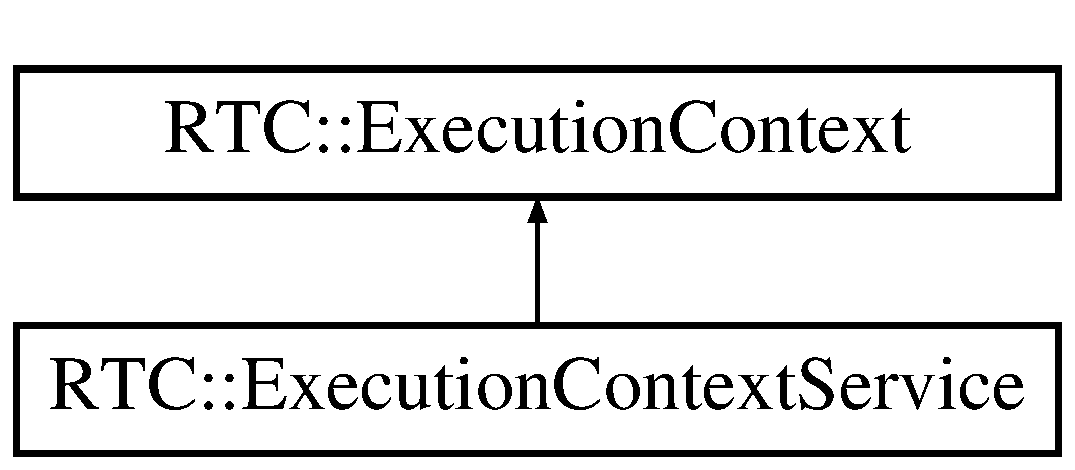
\includegraphics[height=2cm]{interfaceRTC_1_1ExecutionContext}
\end{center}
\end{figure}
\subsection*{Public �᥽�å�}
\begin{CompactItemize}
\item 
boolean {\bf is\_\-running} ()
\item 
{\bf Return\-Code\_\-t} {\bf start} ()
\item 
{\bf Return\-Code\_\-t} {\bf stop} ()
\item 
double {\bf get\_\-rate} ()
\item 
{\bf Return\-Code\_\-t} {\bf set\_\-rate} (in double rate)
\item 
{\bf Return\-Code\_\-t} {\bf activate\_\-component} (in {\bf Lightweight\-RTObject} comp)
\item 
{\bf Return\-Code\_\-t} {\bf deactivate\_\-component} (in {\bf Lightweight\-RTObject} comp)
\item 
{\bf Return\-Code\_\-t} {\bf reset\_\-component} (in {\bf Lightweight\-RTObject} comp)
\item 
{\bf Life\-Cycle\-State} {\bf get\_\-component\_\-state} (in {\bf Lightweight\-RTObject} comp)
\item 
{\bf Execution\-Kind} {\bf get\_\-kind} ()
\item 
{\bf Return\-Code\_\-t} {\bf add} (in {\bf Lightweight\-RTObject} comp)
\item 
{\bf Return\-Code\_\-t} {\bf remove} (in {\bf Lightweight\-RTObject} comp)
\end{CompactItemize}


\subsection{����}
Lightweight\-RTC::Execution\-Context interface. 



\subsection{�ؿ�}
\index{RTC::ExecutionContext@{RTC::Execution\-Context}!activate_component@{activate\_\-component}}
\index{activate_component@{activate\_\-component}!RTC::ExecutionContext@{RTC::Execution\-Context}}
\subsubsection{\setlength{\rightskip}{0pt plus 5cm}{\bf Return\-Code\_\-t} RTC::Execution\-Context::activate\_\-component (in {\bf Lightweight\-RTObject} {\em comp})}\label{interfaceRTC_1_1ExecutionContext_RTC_1_1ExecutionContextServicea6}


\index{RTC::ExecutionContext@{RTC::Execution\-Context}!add@{add}}
\index{add@{add}!RTC::ExecutionContext@{RTC::Execution\-Context}}
\subsubsection{\setlength{\rightskip}{0pt plus 5cm}{\bf Return\-Code\_\-t} RTC::Execution\-Context::add (in {\bf Lightweight\-RTObject} {\em comp})}\label{interfaceRTC_1_1ExecutionContext_RTC_1_1ExecutionContextServicea11}


\index{RTC::ExecutionContext@{RTC::Execution\-Context}!deactivate_component@{deactivate\_\-component}}
\index{deactivate_component@{deactivate\_\-component}!RTC::ExecutionContext@{RTC::Execution\-Context}}
\subsubsection{\setlength{\rightskip}{0pt plus 5cm}{\bf Return\-Code\_\-t} RTC::Execution\-Context::deactivate\_\-component (in {\bf Lightweight\-RTObject} {\em comp})}\label{interfaceRTC_1_1ExecutionContext_RTC_1_1ExecutionContextServicea7}


\index{RTC::ExecutionContext@{RTC::Execution\-Context}!get_component_state@{get\_\-component\_\-state}}
\index{get_component_state@{get\_\-component\_\-state}!RTC::ExecutionContext@{RTC::Execution\-Context}}
\subsubsection{\setlength{\rightskip}{0pt plus 5cm}{\bf Life\-Cycle\-State} RTC::Execution\-Context::get\_\-component\_\-state (in {\bf Lightweight\-RTObject} {\em comp})}\label{interfaceRTC_1_1ExecutionContext_RTC_1_1ExecutionContextServicea9}


\index{RTC::ExecutionContext@{RTC::Execution\-Context}!get_kind@{get\_\-kind}}
\index{get_kind@{get\_\-kind}!RTC::ExecutionContext@{RTC::Execution\-Context}}
\subsubsection{\setlength{\rightskip}{0pt plus 5cm}{\bf Execution\-Kind} RTC::Execution\-Context::get\_\-kind ()}\label{interfaceRTC_1_1ExecutionContext_RTC_1_1ExecutionContextServicea10}


\index{RTC::ExecutionContext@{RTC::Execution\-Context}!get_rate@{get\_\-rate}}
\index{get_rate@{get\_\-rate}!RTC::ExecutionContext@{RTC::Execution\-Context}}
\subsubsection{\setlength{\rightskip}{0pt plus 5cm}double RTC::Execution\-Context::get\_\-rate ()}\label{interfaceRTC_1_1ExecutionContext_RTC_1_1ExecutionContextServicea4}


\index{RTC::ExecutionContext@{RTC::Execution\-Context}!is_running@{is\_\-running}}
\index{is_running@{is\_\-running}!RTC::ExecutionContext@{RTC::Execution\-Context}}
\subsubsection{\setlength{\rightskip}{0pt plus 5cm}boolean RTC::Execution\-Context::is\_\-running ()}\label{interfaceRTC_1_1ExecutionContext_RTC_1_1ExecutionContextServicea1}


\index{RTC::ExecutionContext@{RTC::Execution\-Context}!remove@{remove}}
\index{remove@{remove}!RTC::ExecutionContext@{RTC::Execution\-Context}}
\subsubsection{\setlength{\rightskip}{0pt plus 5cm}{\bf Return\-Code\_\-t} RTC::Execution\-Context::remove (in {\bf Lightweight\-RTObject} {\em comp})}\label{interfaceRTC_1_1ExecutionContext_RTC_1_1ExecutionContextServicea12}


\index{RTC::ExecutionContext@{RTC::Execution\-Context}!reset_component@{reset\_\-component}}
\index{reset_component@{reset\_\-component}!RTC::ExecutionContext@{RTC::Execution\-Context}}
\subsubsection{\setlength{\rightskip}{0pt plus 5cm}{\bf Return\-Code\_\-t} RTC::Execution\-Context::reset\_\-component (in {\bf Lightweight\-RTObject} {\em comp})}\label{interfaceRTC_1_1ExecutionContext_RTC_1_1ExecutionContextServicea8}


\index{RTC::ExecutionContext@{RTC::Execution\-Context}!set_rate@{set\_\-rate}}
\index{set_rate@{set\_\-rate}!RTC::ExecutionContext@{RTC::Execution\-Context}}
\subsubsection{\setlength{\rightskip}{0pt plus 5cm}{\bf Return\-Code\_\-t} RTC::Execution\-Context::set\_\-rate (in double {\em rate})}\label{interfaceRTC_1_1ExecutionContext_RTC_1_1ExecutionContextServicea5}


\index{RTC::ExecutionContext@{RTC::Execution\-Context}!start@{start}}
\index{start@{start}!RTC::ExecutionContext@{RTC::Execution\-Context}}
\subsubsection{\setlength{\rightskip}{0pt plus 5cm}{\bf Return\-Code\_\-t} RTC::Execution\-Context::start ()}\label{interfaceRTC_1_1ExecutionContext_RTC_1_1ExecutionContextServicea2}


\index{RTC::ExecutionContext@{RTC::Execution\-Context}!stop@{stop}}
\index{stop@{stop}!RTC::ExecutionContext@{RTC::Execution\-Context}}
\subsubsection{\setlength{\rightskip}{0pt plus 5cm}{\bf Return\-Code\_\-t} RTC::Execution\-Context::stop ()}\label{interfaceRTC_1_1ExecutionContext_RTC_1_1ExecutionContextServicea3}




���Υ��󥿥ե������������ϼ��Υե����뤫����������ޤ���:\begin{CompactItemize}
\item 
{\bf RTC.idl}\end{CompactItemize}

\section{RTC::Execution\-Context\-Profile Struct Reference}
\label{structRTC_1_1ExecutionContextProfile}\index{RTC::ExecutionContextProfile@{RTC::ExecutionContextProfile}}
Introspection::Execution\-Context\-Profile structure.  


{\tt import \char`\"{}RTC.idl\char`\"{};}

\subsection*{Public Attributes}
\begin{CompactItemize}
\item 
{\bf Execution\-Kind} {\bf kind}
\item 
double {\bf rate}
\item 
{\bf RTObject} {\bf owner}
\item 
{\bf RTCList} {\bf participants}
\item 
{\bf NVList} {\bf properties}
\end{CompactItemize}


\subsection{Detailed Description}
Introspection::Execution\-Context\-Profile structure. 



\subsection{Member Data Documentation}
\index{RTC::ExecutionContextProfile@{RTC::Execution\-Context\-Profile}!kind@{kind}}
\index{kind@{kind}!RTC::ExecutionContextProfile@{RTC::Execution\-Context\-Profile}}
\subsubsection{\setlength{\rightskip}{0pt plus 5cm}{\bf Execution\-Kind} {\bf RTC::Execution\-Context\-Profile::kind}}\label{structRTC_1_1ExecutionContextProfile_RTC_1_1ExecutionContextProfileo0}


\index{RTC::ExecutionContextProfile@{RTC::Execution\-Context\-Profile}!owner@{owner}}
\index{owner@{owner}!RTC::ExecutionContextProfile@{RTC::Execution\-Context\-Profile}}
\subsubsection{\setlength{\rightskip}{0pt plus 5cm}{\bf RTObject} {\bf RTC::Execution\-Context\-Profile::owner}}\label{structRTC_1_1ExecutionContextProfile_RTC_1_1ExecutionContextProfileo2}


\index{RTC::ExecutionContextProfile@{RTC::Execution\-Context\-Profile}!participants@{participants}}
\index{participants@{participants}!RTC::ExecutionContextProfile@{RTC::Execution\-Context\-Profile}}
\subsubsection{\setlength{\rightskip}{0pt plus 5cm}{\bf RTCList} {\bf RTC::Execution\-Context\-Profile::participants}}\label{structRTC_1_1ExecutionContextProfile_RTC_1_1ExecutionContextProfileo3}


\index{RTC::ExecutionContextProfile@{RTC::Execution\-Context\-Profile}!properties@{properties}}
\index{properties@{properties}!RTC::ExecutionContextProfile@{RTC::Execution\-Context\-Profile}}
\subsubsection{\setlength{\rightskip}{0pt plus 5cm}{\bf NVList} {\bf RTC::Execution\-Context\-Profile::properties}}\label{structRTC_1_1ExecutionContextProfile_RTC_1_1ExecutionContextProfileo4}


\index{RTC::ExecutionContextProfile@{RTC::Execution\-Context\-Profile}!rate@{rate}}
\index{rate@{rate}!RTC::ExecutionContextProfile@{RTC::Execution\-Context\-Profile}}
\subsubsection{\setlength{\rightskip}{0pt plus 5cm}double {\bf RTC::Execution\-Context\-Profile::rate}}\label{structRTC_1_1ExecutionContextProfile_RTC_1_1ExecutionContextProfileo1}




The documentation for this struct was generated from the following file:\begin{CompactItemize}
\item 
{\bf RTC.idl}\end{CompactItemize}

\section{RTC::Execution\-Context\-Service Interface Reference}
\label{interfaceRTC_1_1ExecutionContextService}\index{RTC::ExecutionContextService@{RTC::ExecutionContextService}}
Introspection::Execution\-Context\-Service interface.  


{\tt import \char`\"{}RTC.idl\char`\"{};}

Inheritance diagram for RTC::Execution\-Context\-Service::\begin{figure}[H]
\begin{center}
\leavevmode
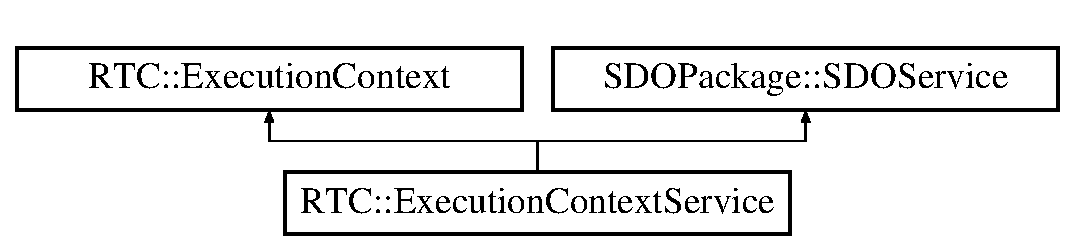
\includegraphics[height=2cm]{interfaceRTC_1_1ExecutionContextService}
\end{center}
\end{figure}
\subsection*{Public Member Functions}
\begin{CompactItemize}
\item 
{\bf Execution\-Context\-Profile} {\bf get\_\-profile} ()
\item 
boolean {\bf is\_\-running} ()
\item 
{\bf Return\-Code\_\-t} {\bf start} ()
\item 
{\bf Return\-Code\_\-t} {\bf stop} ()
\item 
double {\bf get\_\-rate} ()
\item 
{\bf Return\-Code\_\-t} {\bf set\_\-rate} (in double rate)
\item 
{\bf Return\-Code\_\-t} {\bf activate\_\-component} (in {\bf Lightweight\-RTObject} comp)
\item 
{\bf Return\-Code\_\-t} {\bf deactivate\_\-component} (in {\bf Lightweight\-RTObject} comp)
\item 
{\bf Return\-Code\_\-t} {\bf reset\_\-component} (in {\bf Lightweight\-RTObject} comp)
\item 
{\bf Life\-Cycle\-State} {\bf get\_\-component\_\-state} (in {\bf Lightweight\-RTObject} comp)
\item 
{\bf Execution\-Kind} {\bf get\_\-kind} ()
\item 
{\bf Return\-Code\_\-t} {\bf add} (in {\bf Lightweight\-RTObject} comp)
\item 
{\bf Return\-Code\_\-t} {\bf remove} (in {\bf Lightweight\-RTObject} comp)
\end{CompactItemize}


\subsection{Detailed Description}
Introspection::Execution\-Context\-Service interface. 



\subsection{Member Function Documentation}
\index{RTC::ExecutionContextService@{RTC::Execution\-Context\-Service}!activate_component@{activate\_\-component}}
\index{activate_component@{activate\_\-component}!RTC::ExecutionContextService@{RTC::Execution\-Context\-Service}}
\subsubsection{\setlength{\rightskip}{0pt plus 5cm}{\bf Return\-Code\_\-t} RTC::Execution\-Context::activate\_\-component (in {\bf Lightweight\-RTObject} {\em comp})\hspace{0.3cm}{\tt  [inherited]}}\label{interfaceRTC_1_1ExecutionContext_RTC_1_1ExecutionContextServicea6}


\index{RTC::ExecutionContextService@{RTC::Execution\-Context\-Service}!add@{add}}
\index{add@{add}!RTC::ExecutionContextService@{RTC::Execution\-Context\-Service}}
\subsubsection{\setlength{\rightskip}{0pt plus 5cm}{\bf Return\-Code\_\-t} RTC::Execution\-Context::add (in {\bf Lightweight\-RTObject} {\em comp})\hspace{0.3cm}{\tt  [inherited]}}\label{interfaceRTC_1_1ExecutionContext_RTC_1_1ExecutionContextServicea11}


\index{RTC::ExecutionContextService@{RTC::Execution\-Context\-Service}!deactivate_component@{deactivate\_\-component}}
\index{deactivate_component@{deactivate\_\-component}!RTC::ExecutionContextService@{RTC::Execution\-Context\-Service}}
\subsubsection{\setlength{\rightskip}{0pt plus 5cm}{\bf Return\-Code\_\-t} RTC::Execution\-Context::deactivate\_\-component (in {\bf Lightweight\-RTObject} {\em comp})\hspace{0.3cm}{\tt  [inherited]}}\label{interfaceRTC_1_1ExecutionContext_RTC_1_1ExecutionContextServicea7}


\index{RTC::ExecutionContextService@{RTC::Execution\-Context\-Service}!get_component_state@{get\_\-component\_\-state}}
\index{get_component_state@{get\_\-component\_\-state}!RTC::ExecutionContextService@{RTC::Execution\-Context\-Service}}
\subsubsection{\setlength{\rightskip}{0pt plus 5cm}{\bf Life\-Cycle\-State} RTC::Execution\-Context::get\_\-component\_\-state (in {\bf Lightweight\-RTObject} {\em comp})\hspace{0.3cm}{\tt  [inherited]}}\label{interfaceRTC_1_1ExecutionContext_RTC_1_1ExecutionContextServicea9}


\index{RTC::ExecutionContextService@{RTC::Execution\-Context\-Service}!get_kind@{get\_\-kind}}
\index{get_kind@{get\_\-kind}!RTC::ExecutionContextService@{RTC::Execution\-Context\-Service}}
\subsubsection{\setlength{\rightskip}{0pt plus 5cm}{\bf Execution\-Kind} RTC::Execution\-Context::get\_\-kind ()\hspace{0.3cm}{\tt  [inherited]}}\label{interfaceRTC_1_1ExecutionContext_RTC_1_1ExecutionContextServicea10}


\index{RTC::ExecutionContextService@{RTC::Execution\-Context\-Service}!get_profile@{get\_\-profile}}
\index{get_profile@{get\_\-profile}!RTC::ExecutionContextService@{RTC::Execution\-Context\-Service}}
\subsubsection{\setlength{\rightskip}{0pt plus 5cm}{\bf Execution\-Context\-Profile} RTC::Execution\-Context\-Service::get\_\-profile ()}\label{interfaceRTC_1_1ExecutionContextService_RTC_1_1ExecutionContextServicea0}


\index{RTC::ExecutionContextService@{RTC::Execution\-Context\-Service}!get_rate@{get\_\-rate}}
\index{get_rate@{get\_\-rate}!RTC::ExecutionContextService@{RTC::Execution\-Context\-Service}}
\subsubsection{\setlength{\rightskip}{0pt plus 5cm}double RTC::Execution\-Context::get\_\-rate ()\hspace{0.3cm}{\tt  [inherited]}}\label{interfaceRTC_1_1ExecutionContext_RTC_1_1ExecutionContextServicea4}


\index{RTC::ExecutionContextService@{RTC::Execution\-Context\-Service}!is_running@{is\_\-running}}
\index{is_running@{is\_\-running}!RTC::ExecutionContextService@{RTC::Execution\-Context\-Service}}
\subsubsection{\setlength{\rightskip}{0pt plus 5cm}boolean RTC::Execution\-Context::is\_\-running ()\hspace{0.3cm}{\tt  [inherited]}}\label{interfaceRTC_1_1ExecutionContext_RTC_1_1ExecutionContextServicea1}


\index{RTC::ExecutionContextService@{RTC::Execution\-Context\-Service}!remove@{remove}}
\index{remove@{remove}!RTC::ExecutionContextService@{RTC::Execution\-Context\-Service}}
\subsubsection{\setlength{\rightskip}{0pt plus 5cm}{\bf Return\-Code\_\-t} RTC::Execution\-Context::remove (in {\bf Lightweight\-RTObject} {\em comp})\hspace{0.3cm}{\tt  [inherited]}}\label{interfaceRTC_1_1ExecutionContext_RTC_1_1ExecutionContextServicea12}


\index{RTC::ExecutionContextService@{RTC::Execution\-Context\-Service}!reset_component@{reset\_\-component}}
\index{reset_component@{reset\_\-component}!RTC::ExecutionContextService@{RTC::Execution\-Context\-Service}}
\subsubsection{\setlength{\rightskip}{0pt plus 5cm}{\bf Return\-Code\_\-t} RTC::Execution\-Context::reset\_\-component (in {\bf Lightweight\-RTObject} {\em comp})\hspace{0.3cm}{\tt  [inherited]}}\label{interfaceRTC_1_1ExecutionContext_RTC_1_1ExecutionContextServicea8}


\index{RTC::ExecutionContextService@{RTC::Execution\-Context\-Service}!set_rate@{set\_\-rate}}
\index{set_rate@{set\_\-rate}!RTC::ExecutionContextService@{RTC::Execution\-Context\-Service}}
\subsubsection{\setlength{\rightskip}{0pt plus 5cm}{\bf Return\-Code\_\-t} RTC::Execution\-Context::set\_\-rate (in double {\em rate})\hspace{0.3cm}{\tt  [inherited]}}\label{interfaceRTC_1_1ExecutionContext_RTC_1_1ExecutionContextServicea5}


\index{RTC::ExecutionContextService@{RTC::Execution\-Context\-Service}!start@{start}}
\index{start@{start}!RTC::ExecutionContextService@{RTC::Execution\-Context\-Service}}
\subsubsection{\setlength{\rightskip}{0pt plus 5cm}{\bf Return\-Code\_\-t} RTC::Execution\-Context::start ()\hspace{0.3cm}{\tt  [inherited]}}\label{interfaceRTC_1_1ExecutionContext_RTC_1_1ExecutionContextServicea2}


\index{RTC::ExecutionContextService@{RTC::Execution\-Context\-Service}!stop@{stop}}
\index{stop@{stop}!RTC::ExecutionContextService@{RTC::Execution\-Context\-Service}}
\subsubsection{\setlength{\rightskip}{0pt plus 5cm}{\bf Return\-Code\_\-t} RTC::Execution\-Context::stop ()\hspace{0.3cm}{\tt  [inherited]}}\label{interfaceRTC_1_1ExecutionContext_RTC_1_1ExecutionContextServicea3}




The documentation for this interface was generated from the following file:\begin{CompactItemize}
\item 
{\bf RTC.idl}\end{CompactItemize}

\section{��¤�� RTC::Fsm\-Bihavior\-Profile}
\label{structRTC_1_1FsmBihaviorProfile}\index{RTC::FsmBihaviorProfile@{RTC::FsmBihaviorProfile}}
Introspection::Fsm\-Bihavior\-Profile structure.  


{\tt import \char`\"{}RTC.idl\char`\"{};}

\subsection*{Public �ѿ�}
\begin{CompactItemize}
\item 
{\bf Unique\-Identifier} {\bf id}
\item 
{\bf Fsm\-Participant\-Action} {\bf comp}
\end{CompactItemize}


\subsection{����}
Introspection::Fsm\-Bihavior\-Profile structure. 



\subsection{�ѿ�}
\index{RTC::FsmBihaviorProfile@{RTC::Fsm\-Bihavior\-Profile}!comp@{comp}}
\index{comp@{comp}!RTC::FsmBihaviorProfile@{RTC::Fsm\-Bihavior\-Profile}}
\subsubsection{\setlength{\rightskip}{0pt plus 5cm}{\bf Fsm\-Participant\-Action} {\bf RTC::Fsm\-Bihavior\-Profile::comp}}\label{structRTC_1_1FsmBihaviorProfile_RTC_1_1FsmBihaviorProfileo1}


\index{RTC::FsmBihaviorProfile@{RTC::Fsm\-Bihavior\-Profile}!id@{id}}
\index{id@{id}!RTC::FsmBihaviorProfile@{RTC::Fsm\-Bihavior\-Profile}}
\subsubsection{\setlength{\rightskip}{0pt plus 5cm}{\bf Unique\-Identifier} {\bf RTC::Fsm\-Bihavior\-Profile::id}}\label{structRTC_1_1FsmBihaviorProfile_RTC_1_1FsmBihaviorProfileo0}




���ι�¤�Τ������ϼ��Υե����뤫����������ޤ���:\begin{CompactItemize}
\item 
{\bf RTC.idl}\end{CompactItemize}

\section{RTC::Fsm\-Object Interface Reference}
\label{interfaceRTC_1_1FsmObject}\index{RTC::FsmObject@{RTC::FsmObject}}
Execution\-Semantics::Fsm\-Object interface.  


{\tt import \char`\"{}RTC.idl\char`\"{};}

\subsection*{Public Member Functions}
\begin{CompactItemize}
\item 
{\bf Return\-Code\_\-t} {\bf stimulate} (in string message, in {\bf Unique\-Id} ec\_\-id)
\end{CompactItemize}


\subsection{Detailed Description}
Execution\-Semantics::Fsm\-Object interface. 



\subsection{Member Function Documentation}
\index{RTC::FsmObject@{RTC::Fsm\-Object}!stimulate@{stimulate}}
\index{stimulate@{stimulate}!RTC::FsmObject@{RTC::Fsm\-Object}}
\subsubsection{\setlength{\rightskip}{0pt plus 5cm}{\bf Return\-Code\_\-t} RTC::Fsm\-Object::stimulate (in string {\em message}, in {\bf Unique\-Id} {\em ec\_\-id})}\label{interfaceRTC_1_1FsmObject_RTC_1_1FsmObjecta0}




The documentation for this interface was generated from the following file:\begin{CompactItemize}
\item 
{\bf RTC.idl}\end{CompactItemize}

\section{���󥿥ե����� RTC::Fsm\-Participant}
\label{interfaceRTC_1_1FsmParticipant}\index{RTC::FsmParticipant@{RTC::FsmParticipant}}
Execution\-Semantics::Fsm\-Participant component.  


{\tt import \char`\"{}RTC.idl\char`\"{};}

RTC::Fsm\-Participant���Ф���Ѿ������:\begin{figure}[H]
\begin{center}
\leavevmode
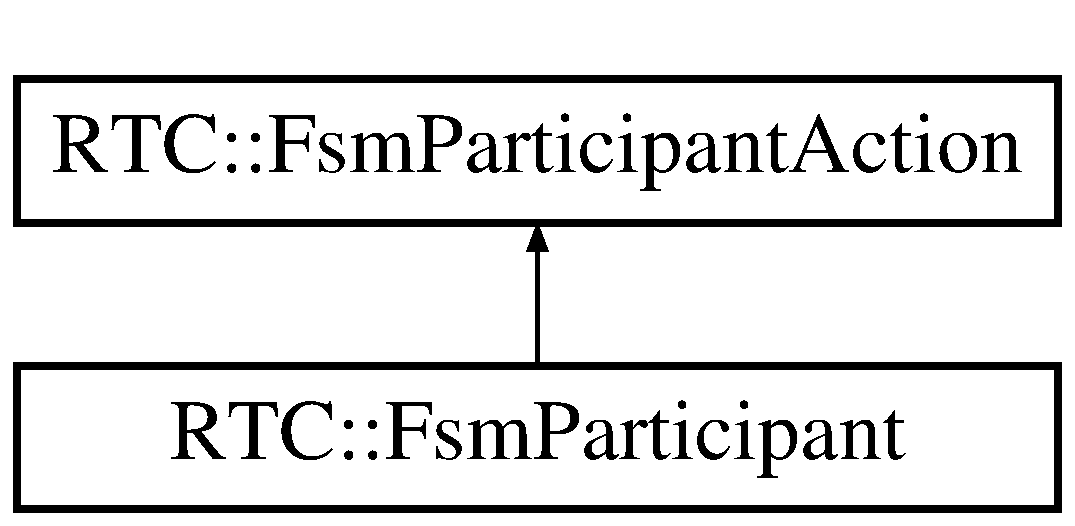
\includegraphics[height=2cm]{interfaceRTC_1_1FsmParticipant}
\end{center}
\end{figure}
\subsection*{Public �᥽�å�}
\begin{CompactItemize}
\item 
{\bf Return\-Code\_\-t} {\bf on\_\-action} (in {\bf Unique\-Id} ec\_\-id)
\end{CompactItemize}


\subsection{����}
Execution\-Semantics::Fsm\-Participant component. 



\subsection{�ؿ�}
\index{RTC::FsmParticipant@{RTC::Fsm\-Participant}!on_action@{on\_\-action}}
\index{on_action@{on\_\-action}!RTC::FsmParticipant@{RTC::Fsm\-Participant}}
\subsubsection{\setlength{\rightskip}{0pt plus 5cm}{\bf Return\-Code\_\-t} RTC::Fsm\-Participant\-Action::on\_\-action (in {\bf Unique\-Id} {\em ec\_\-id})\hspace{0.3cm}{\tt  [inherited]}}\label{interfaceRTC_1_1FsmParticipantAction_RTC_1_1FsmParticipantActiona0}




���Υ��󥿥ե������������ϼ��Υե����뤫����������ޤ���:\begin{CompactItemize}
\item 
{\bf RTC.idl}\end{CompactItemize}

\section{RTC::Fsm\-Participant\-Action Interface Reference}
\label{interfaceRTC_1_1FsmParticipantAction}\index{RTC::FsmParticipantAction@{RTC::FsmParticipantAction}}
Execution\-Semantics::Fsm\-Participant\-Action interface.  


{\tt import \char`\"{}RTC.idl\char`\"{};}

Inheritance diagram for RTC::Fsm\-Participant\-Action::\begin{figure}[H]
\begin{center}
\leavevmode
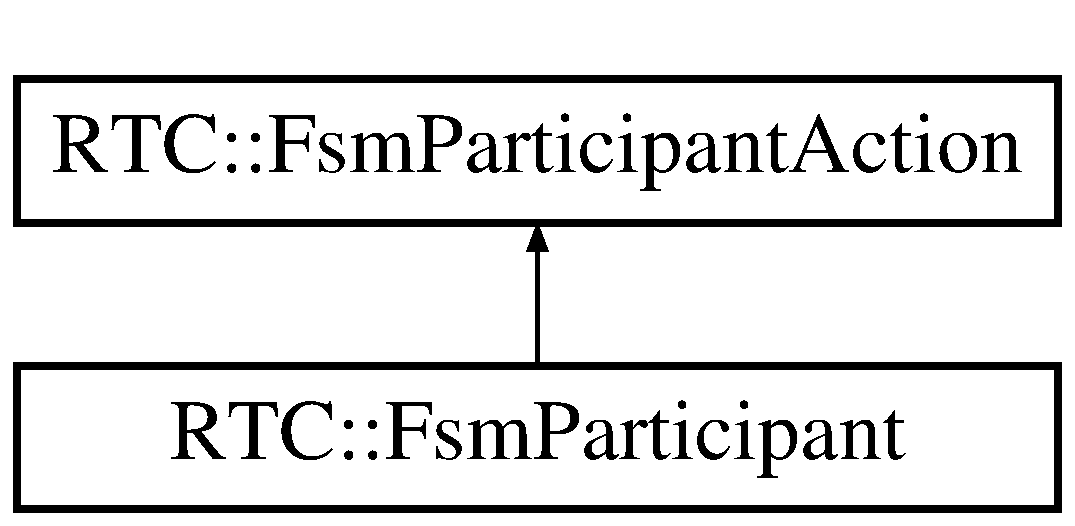
\includegraphics[height=2cm]{interfaceRTC_1_1FsmParticipantAction}
\end{center}
\end{figure}
\subsection*{Public Member Functions}
\begin{CompactItemize}
\item 
{\bf Return\-Code\_\-t} {\bf on\_\-action} (in {\bf Unique\-Id} ec\_\-id)
\end{CompactItemize}


\subsection{Detailed Description}
Execution\-Semantics::Fsm\-Participant\-Action interface. 



\subsection{Member Function Documentation}
\index{RTC::FsmParticipantAction@{RTC::Fsm\-Participant\-Action}!on_action@{on\_\-action}}
\index{on_action@{on\_\-action}!RTC::FsmParticipantAction@{RTC::Fsm\-Participant\-Action}}
\subsubsection{\setlength{\rightskip}{0pt plus 5cm}{\bf Return\-Code\_\-t} RTC::Fsm\-Participant\-Action::on\_\-action (in {\bf Unique\-Id} {\em ec\_\-id})}\label{interfaceRTC_1_1FsmParticipantAction_RTC_1_1FsmParticipantActiona0}




The documentation for this interface was generated from the following file:\begin{CompactItemize}
\item 
{\bf RTC.idl}\end{CompactItemize}

\section{RTC::Fsm\-Profile Struct Reference}
\label{structRTC_1_1FsmProfile}\index{RTC::FsmProfile@{RTC::FsmProfile}}
Introspection::Fsm\-Profile structure.  


{\tt import \char`\"{}RTC.idl\char`\"{};}

\subsection*{Public Attributes}
\begin{CompactItemize}
\item 
sequence$<$ {\bf Fsm\-Bihavior\-Profile} $>$ {\bf bihavior\_\-profiles}
\end{CompactItemize}


\subsection{Detailed Description}
Introspection::Fsm\-Profile structure. 



\subsection{Member Data Documentation}
\index{RTC::FsmProfile@{RTC::Fsm\-Profile}!bihavior_profiles@{bihavior\_\-profiles}}
\index{bihavior_profiles@{bihavior\_\-profiles}!RTC::FsmProfile@{RTC::Fsm\-Profile}}
\subsubsection{\setlength{\rightskip}{0pt plus 5cm}sequence$<${\bf Fsm\-Bihavior\-Profile}$>$ {\bf RTC::Fsm\-Profile::bihavior\_\-profiles}}\label{structRTC_1_1FsmProfile_RTC_1_1FsmProfileo0}




The documentation for this struct was generated from the following file:\begin{CompactItemize}
\item 
{\bf RTC.idl}\end{CompactItemize}

\section{���󥿥ե����� RTC::Fsm\-Service}
\label{interfaceRTC_1_1FsmService}\index{RTC::FsmService@{RTC::FsmService}}
Introspection::Fsm\-Service interface.  


{\tt import \char`\"{}RTC.idl\char`\"{};}

RTC::Fsm\-Service���Ф���Ѿ������:\begin{figure}[H]
\begin{center}
\leavevmode
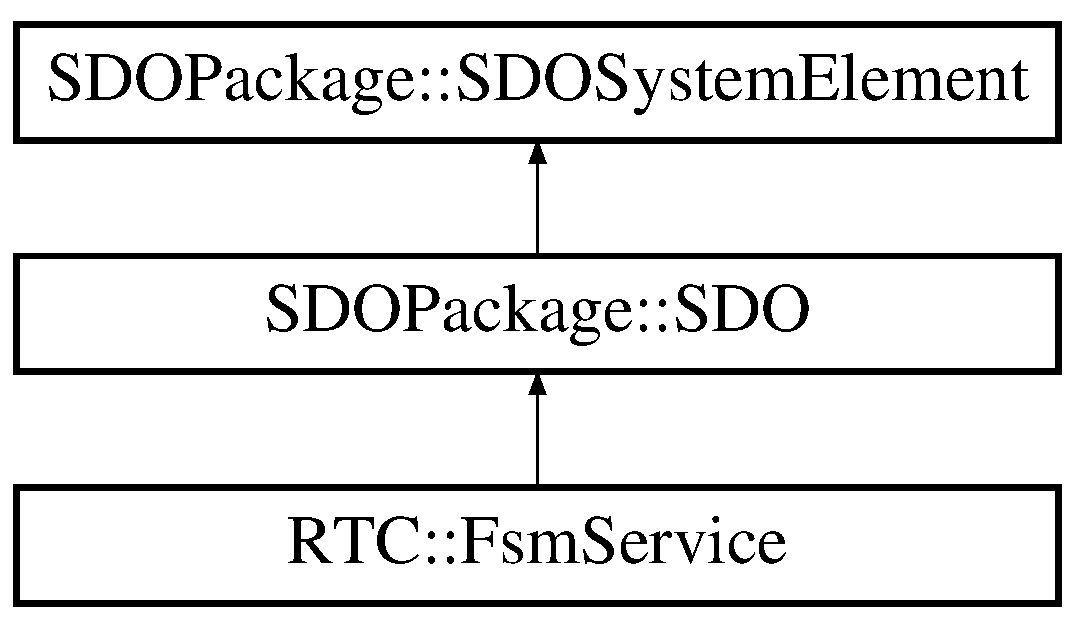
\includegraphics[height=3cm]{interfaceRTC_1_1FsmService}
\end{center}
\end{figure}
\subsection*{Public �᥽�å�}
\begin{CompactItemize}
\item 
{\bf Fsm\-Profile} {\bf get\_\-fsm\_\-profile} ()
\item 
{\bf Return\-Code\_\-t} {\bf set\_\-fsm\_\-profile} ()
\item 
{\bf Unique\-Identifier} {\bf get\_\-sdo\_\-id} ()  raises (Not\-Available, Internal\-Error)
\item 
string {\bf get\_\-sdo\_\-type} ()  raises (Not\-Available, Internal\-Error)
\item 
Device\-Profile {\bf get\_\-device\_\-profile} ()  raises (Not\-Available, Internal\-Error)
\item 
{\bf Service\-Profile\-List} {\bf get\_\-service\_\-profiles} ()  raises (Not\-Available, Internal\-Error)
\item 
Service\-Profile {\bf get\_\-service\_\-profile} (in {\bf Unique\-Identifier} id)  raises (Invalid\-Parameter, Not\-Available, Internal\-Error)
\item 
SDOService {\bf get\_\-sdo\_\-service} (in {\bf Unique\-Identifier} id)  raises (Invalid\-Parameter, Not\-Available, Internal\-Error)
\item 
Configuration {\bf get\_\-configuration} ()  raises (Interface\-Not\-Implemented, Not\-Available, Internal\-Error)
\item 
Monitoring {\bf get\_\-monitoring} ()  raises (Interface\-Not\-Implemented, Not\-Available, Internal\-Error)
\item 
{\bf Organization\-List} {\bf get\_\-organizations} ()  raises (Not\-Available, Internal\-Error)
\item 
{\bf NVList} {\bf get\_\-status\_\-list} ()  raises (Not\-Available, Internal\-Error)
\item 
any {\bf get\_\-status} (in string name)  raises (Invalid\-Parameter, Not\-Available, Internal\-Error)
\item 
{\bf Organization\-List} {\bf get\_\-owned\_\-organizations} ()  raises (Not\-Available)
\end{CompactItemize}


\subsection{����}
Introspection::Fsm\-Service interface. 



\subsection{�ؿ�}
\index{RTC::FsmService@{RTC::Fsm\-Service}!get_configuration@{get\_\-configuration}}
\index{get_configuration@{get\_\-configuration}!RTC::FsmService@{RTC::Fsm\-Service}}
\subsubsection{\setlength{\rightskip}{0pt plus 5cm}Configuration SDOPackage::SDO::get\_\-configuration ()  raises (Interface\-Not\-Implemented, Not\-Available, Internal\-Error)\hspace{0.3cm}{\tt  [inherited]}}\label{interfaceSDOPackage_1_1SDO_SDOPackage_1_1SDOa6}


\index{RTC::FsmService@{RTC::Fsm\-Service}!get_device_profile@{get\_\-device\_\-profile}}
\index{get_device_profile@{get\_\-device\_\-profile}!RTC::FsmService@{RTC::Fsm\-Service}}
\subsubsection{\setlength{\rightskip}{0pt plus 5cm}Device\-Profile SDOPackage::SDO::get\_\-device\_\-profile ()  raises (Not\-Available, Internal\-Error)\hspace{0.3cm}{\tt  [inherited]}}\label{interfaceSDOPackage_1_1SDO_SDOPackage_1_1SDOa2}


\index{RTC::FsmService@{RTC::Fsm\-Service}!get_fsm_profile@{get\_\-fsm\_\-profile}}
\index{get_fsm_profile@{get\_\-fsm\_\-profile}!RTC::FsmService@{RTC::Fsm\-Service}}
\subsubsection{\setlength{\rightskip}{0pt plus 5cm}{\bf Fsm\-Profile} RTC::Fsm\-Service::get\_\-fsm\_\-profile ()}\label{interfaceRTC_1_1FsmService_RTC_1_1FsmServicea0}


\index{RTC::FsmService@{RTC::Fsm\-Service}!get_monitoring@{get\_\-monitoring}}
\index{get_monitoring@{get\_\-monitoring}!RTC::FsmService@{RTC::Fsm\-Service}}
\subsubsection{\setlength{\rightskip}{0pt plus 5cm}Monitoring SDOPackage::SDO::get\_\-monitoring ()  raises (Interface\-Not\-Implemented, Not\-Available, Internal\-Error)\hspace{0.3cm}{\tt  [inherited]}}\label{interfaceSDOPackage_1_1SDO_SDOPackage_1_1SDOa7}


\index{RTC::FsmService@{RTC::Fsm\-Service}!get_organizations@{get\_\-organizations}}
\index{get_organizations@{get\_\-organizations}!RTC::FsmService@{RTC::Fsm\-Service}}
\subsubsection{\setlength{\rightskip}{0pt plus 5cm}{\bf Organization\-List} SDOPackage::SDO::get\_\-organizations ()  raises (Not\-Available, Internal\-Error)\hspace{0.3cm}{\tt  [inherited]}}\label{interfaceSDOPackage_1_1SDO_SDOPackage_1_1SDOa8}


\index{RTC::FsmService@{RTC::Fsm\-Service}!get_owned_organizations@{get\_\-owned\_\-organizations}}
\index{get_owned_organizations@{get\_\-owned\_\-organizations}!RTC::FsmService@{RTC::Fsm\-Service}}
\subsubsection{\setlength{\rightskip}{0pt plus 5cm}{\bf Organization\-List} SDOPackage::SDOSystem\-Element::get\_\-owned\_\-organizations ()  raises (Not\-Available)\hspace{0.3cm}{\tt  [inherited]}}\label{interfaceSDOPackage_1_1SDOSystemElement_SDOPackage_1_1SDOSystemElementa0}


\index{RTC::FsmService@{RTC::Fsm\-Service}!get_sdo_id@{get\_\-sdo\_\-id}}
\index{get_sdo_id@{get\_\-sdo\_\-id}!RTC::FsmService@{RTC::Fsm\-Service}}
\subsubsection{\setlength{\rightskip}{0pt plus 5cm}{\bf Unique\-Identifier} SDOPackage::SDO::get\_\-sdo\_\-id ()  raises (Not\-Available, Internal\-Error)\hspace{0.3cm}{\tt  [inherited]}}\label{interfaceSDOPackage_1_1SDO_SDOPackage_1_1SDOa0}


\index{RTC::FsmService@{RTC::Fsm\-Service}!get_sdo_service@{get\_\-sdo\_\-service}}
\index{get_sdo_service@{get\_\-sdo\_\-service}!RTC::FsmService@{RTC::Fsm\-Service}}
\subsubsection{\setlength{\rightskip}{0pt plus 5cm}SDOService SDOPackage::SDO::get\_\-sdo\_\-service (in {\bf Unique\-Identifier} {\em id})  raises (Invalid\-Parameter, Not\-Available, Internal\-Error)\hspace{0.3cm}{\tt  [inherited]}}\label{interfaceSDOPackage_1_1SDO_SDOPackage_1_1SDOa5}


\index{RTC::FsmService@{RTC::Fsm\-Service}!get_sdo_type@{get\_\-sdo\_\-type}}
\index{get_sdo_type@{get\_\-sdo\_\-type}!RTC::FsmService@{RTC::Fsm\-Service}}
\subsubsection{\setlength{\rightskip}{0pt plus 5cm}string SDOPackage::SDO::get\_\-sdo\_\-type ()  raises (Not\-Available, Internal\-Error)\hspace{0.3cm}{\tt  [inherited]}}\label{interfaceSDOPackage_1_1SDO_SDOPackage_1_1SDOa1}


\index{RTC::FsmService@{RTC::Fsm\-Service}!get_service_profile@{get\_\-service\_\-profile}}
\index{get_service_profile@{get\_\-service\_\-profile}!RTC::FsmService@{RTC::Fsm\-Service}}
\subsubsection{\setlength{\rightskip}{0pt plus 5cm}Service\-Profile SDOPackage::SDO::get\_\-service\_\-profile (in {\bf Unique\-Identifier} {\em id})  raises (Invalid\-Parameter, Not\-Available, Internal\-Error)\hspace{0.3cm}{\tt  [inherited]}}\label{interfaceSDOPackage_1_1SDO_SDOPackage_1_1SDOa4}


\index{RTC::FsmService@{RTC::Fsm\-Service}!get_service_profiles@{get\_\-service\_\-profiles}}
\index{get_service_profiles@{get\_\-service\_\-profiles}!RTC::FsmService@{RTC::Fsm\-Service}}
\subsubsection{\setlength{\rightskip}{0pt plus 5cm}{\bf Service\-Profile\-List} SDOPackage::SDO::get\_\-service\_\-profiles ()  raises (Not\-Available, Internal\-Error)\hspace{0.3cm}{\tt  [inherited]}}\label{interfaceSDOPackage_1_1SDO_SDOPackage_1_1SDOa3}


\index{RTC::FsmService@{RTC::Fsm\-Service}!get_status@{get\_\-status}}
\index{get_status@{get\_\-status}!RTC::FsmService@{RTC::Fsm\-Service}}
\subsubsection{\setlength{\rightskip}{0pt plus 5cm}any SDOPackage::SDO::get\_\-status (in string {\em name})  raises (Invalid\-Parameter, Not\-Available, Internal\-Error)\hspace{0.3cm}{\tt  [inherited]}}\label{interfaceSDOPackage_1_1SDO_SDOPackage_1_1SDOa10}


\index{RTC::FsmService@{RTC::Fsm\-Service}!get_status_list@{get\_\-status\_\-list}}
\index{get_status_list@{get\_\-status\_\-list}!RTC::FsmService@{RTC::Fsm\-Service}}
\subsubsection{\setlength{\rightskip}{0pt plus 5cm}{\bf NVList} SDOPackage::SDO::get\_\-status\_\-list ()  raises (Not\-Available, Internal\-Error)\hspace{0.3cm}{\tt  [inherited]}}\label{interfaceSDOPackage_1_1SDO_SDOPackage_1_1SDOa9}


\index{RTC::FsmService@{RTC::Fsm\-Service}!set_fsm_profile@{set\_\-fsm\_\-profile}}
\index{set_fsm_profile@{set\_\-fsm\_\-profile}!RTC::FsmService@{RTC::Fsm\-Service}}
\subsubsection{\setlength{\rightskip}{0pt plus 5cm}{\bf Return\-Code\_\-t} RTC::Fsm\-Service::set\_\-fsm\_\-profile ()}\label{interfaceRTC_1_1FsmService_RTC_1_1FsmServicea1}




���Υ��󥿥ե������������ϼ��Υե����뤫����������ޤ���:\begin{CompactItemize}
\item 
{\bf RTC.idl}\end{CompactItemize}

\section{���󥿥ե����� RTC::In\-Port\-Any}
\label{interfaceRTC_1_1InPortAny}\index{RTC::InPortAny@{RTC::InPortAny}}
{\tt import \char`\"{}Data\-Port.idl\char`\"{};}

\subsection*{Public �᥽�å�}
\begin{CompactItemize}
\item 
oneway void {\bf put} (in any data)
\end{CompactItemize}


\subsection{�ؿ�}
\index{RTC::InPortAny@{RTC::In\-Port\-Any}!put@{put}}
\index{put@{put}!RTC::InPortAny@{RTC::In\-Port\-Any}}
\subsubsection{\setlength{\rightskip}{0pt plus 5cm}oneway void RTC::In\-Port\-Any::put (in any {\em data})}\label{interfaceRTC_1_1InPortAny_RTC_1_1InPortAnya0}




���Υ��󥿥ե������������ϼ��Υե����뤫����������ޤ���:\begin{CompactItemize}
\item 
{\bf Data\-Port.idl}\end{CompactItemize}

\section{SDOPackage::Interval\-Type Struct Reference}
\label{structSDOPackage_1_1IntervalType}\index{SDOPackage::IntervalType@{SDOPackage::IntervalType}}
{\tt import \char`\"{}SDOPackage.idl\char`\"{};}

\subsection*{Public Attributes}
\begin{CompactItemize}
\item 
{\bf Numeric} {\bf min}
\item 
{\bf Numeric} {\bf max}
\item 
boolean {\bf min\_\-inclusive}
\item 
boolean {\bf max\_\-inclusive}
\item 
{\bf Numeric} {\bf step}
\end{CompactItemize}


\subsection{Member Data Documentation}
\index{SDOPackage::IntervalType@{SDOPackage::Interval\-Type}!max@{max}}
\index{max@{max}!SDOPackage::IntervalType@{SDOPackage::Interval\-Type}}
\subsubsection{\setlength{\rightskip}{0pt plus 5cm}{\bf Numeric} {\bf SDOPackage::Interval\-Type::max}}\label{structSDOPackage_1_1IntervalType_SDOPackage_1_1IntervalTypeo1}


\index{SDOPackage::IntervalType@{SDOPackage::Interval\-Type}!max_inclusive@{max\_\-inclusive}}
\index{max_inclusive@{max\_\-inclusive}!SDOPackage::IntervalType@{SDOPackage::Interval\-Type}}
\subsubsection{\setlength{\rightskip}{0pt plus 5cm}boolean {\bf SDOPackage::Interval\-Type::max\_\-inclusive}}\label{structSDOPackage_1_1IntervalType_SDOPackage_1_1IntervalTypeo3}


\index{SDOPackage::IntervalType@{SDOPackage::Interval\-Type}!min@{min}}
\index{min@{min}!SDOPackage::IntervalType@{SDOPackage::Interval\-Type}}
\subsubsection{\setlength{\rightskip}{0pt plus 5cm}{\bf Numeric} {\bf SDOPackage::Interval\-Type::min}}\label{structSDOPackage_1_1IntervalType_SDOPackage_1_1IntervalTypeo0}


\index{SDOPackage::IntervalType@{SDOPackage::Interval\-Type}!min_inclusive@{min\_\-inclusive}}
\index{min_inclusive@{min\_\-inclusive}!SDOPackage::IntervalType@{SDOPackage::Interval\-Type}}
\subsubsection{\setlength{\rightskip}{0pt plus 5cm}boolean {\bf SDOPackage::Interval\-Type::min\_\-inclusive}}\label{structSDOPackage_1_1IntervalType_SDOPackage_1_1IntervalTypeo2}


\index{SDOPackage::IntervalType@{SDOPackage::Interval\-Type}!step@{step}}
\index{step@{step}!SDOPackage::IntervalType@{SDOPackage::Interval\-Type}}
\subsubsection{\setlength{\rightskip}{0pt plus 5cm}{\bf Numeric} {\bf SDOPackage::Interval\-Type::step}}\label{structSDOPackage_1_1IntervalType_SDOPackage_1_1IntervalTypeo4}




The documentation for this struct was generated from the following file:\begin{CompactItemize}
\item 
{\bf SDOPackage.idl}\end{CompactItemize}

\section{RTC::Lightweight\-RTObject Interface Reference}
\label{interfaceRTC_1_1LightweightRTObject}\index{RTC::LightweightRTObject@{RTC::LightweightRTObject}}
Lightweight\-RTC::Lightweight\-RTObject interface.  


{\tt import \char`\"{}RTC.idl\char`\"{};}

Inheritance diagram for RTC::Lightweight\-RTObject::\begin{figure}[H]
\begin{center}
\leavevmode
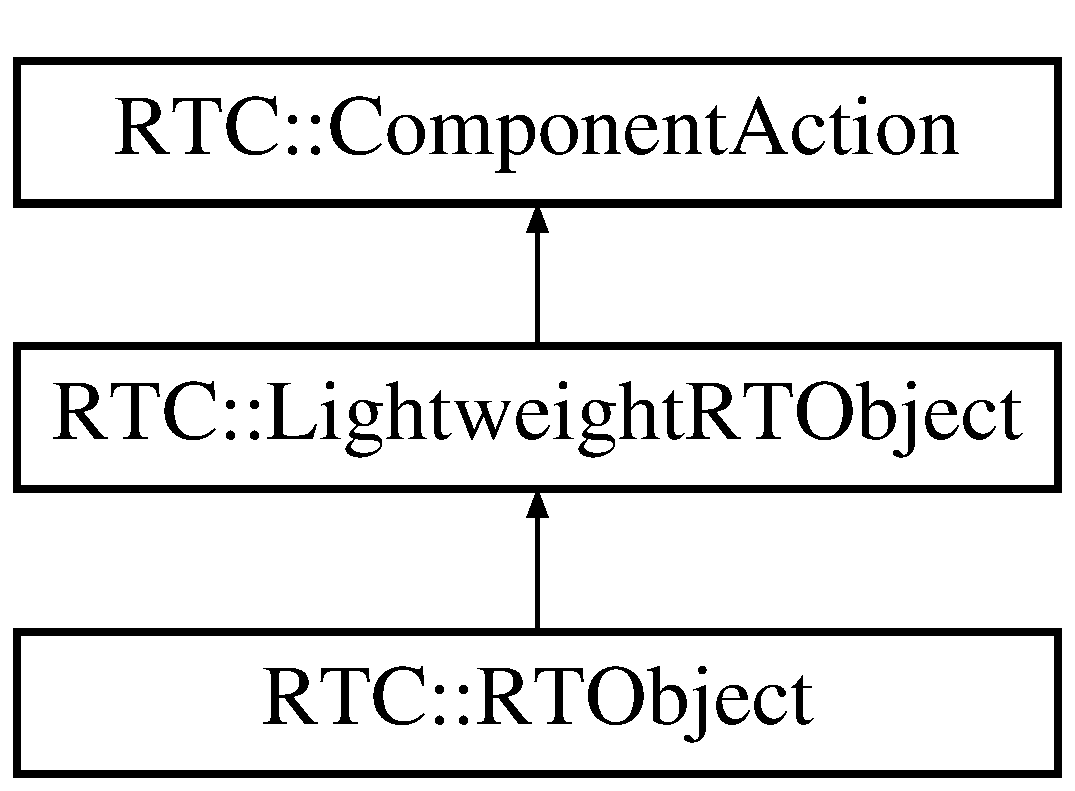
\includegraphics[height=3cm]{interfaceRTC_1_1LightweightRTObject}
\end{center}
\end{figure}
\subsection*{Public Member Functions}
\begin{CompactItemize}
\item 
{\bf Return\-Code\_\-t} {\bf initialize} ()
\item 
{\bf Return\-Code\_\-t} {\bf finalize} ()
\item 
{\bf Return\-Code\_\-t} {\bf exit} ()
\item 
boolean {\bf is\_\-alive} ()
\item 
{\bf Execution\-Context\-List} {\bf get\_\-contexts} ()
\item 
{\bf Execution\-Context} {\bf get\_\-context} (in {\bf Unique\-Id} ec\_\-id)
\item 
{\bf Unique\-Id} {\bf attach\_\-executioncontext} (in {\bf Execution\-Context} exec\_\-context)
\item 
{\bf Return\-Code\_\-t} {\bf detach\_\-executioncontext} (in {\bf Unique\-Id} ec\_\-id)
\item 
{\bf Return\-Code\_\-t} {\bf on\_\-initialize} ()
\item 
{\bf Return\-Code\_\-t} {\bf on\_\-finalize} ()
\item 
{\bf Return\-Code\_\-t} {\bf on\_\-startup} (in {\bf Unique\-Id} ec\_\-id)
\item 
{\bf Return\-Code\_\-t} {\bf on\_\-shutdown} (in {\bf Unique\-Id} ec\_\-id)
\item 
{\bf Return\-Code\_\-t} {\bf on\_\-activated} (in {\bf Unique\-Id} ec\_\-id)
\item 
{\bf Return\-Code\_\-t} {\bf on\_\-deactivated} (in {\bf Unique\-Id} ec\_\-id)
\item 
{\bf Return\-Code\_\-t} {\bf on\_\-aborting} (in {\bf Unique\-Id} ec\_\-id)
\item 
{\bf Return\-Code\_\-t} {\bf on\_\-error} (in {\bf Unique\-Id} ec\_\-id)
\item 
{\bf Return\-Code\_\-t} {\bf on\_\-reset} (in {\bf Unique\-Id} ec\_\-id)
\end{CompactItemize}


\subsection{Detailed Description}
Lightweight\-RTC::Lightweight\-RTObject interface. 



\subsection{Member Function Documentation}
\index{RTC::LightweightRTObject@{RTC::Lightweight\-RTObject}!attach_executioncontext@{attach\_\-executioncontext}}
\index{attach_executioncontext@{attach\_\-executioncontext}!RTC::LightweightRTObject@{RTC::Lightweight\-RTObject}}
\subsubsection{\setlength{\rightskip}{0pt plus 5cm}{\bf Unique\-Id} RTC::Component\-Action::attach\_\-executioncontext (in {\bf Execution\-Context} {\em exec\_\-context})\hspace{0.3cm}{\tt  [inherited]}}\label{interfaceRTC_1_1ComponentAction_RTC_1_1RTObjecta9}


\index{RTC::LightweightRTObject@{RTC::Lightweight\-RTObject}!detach_executioncontext@{detach\_\-executioncontext}}
\index{detach_executioncontext@{detach\_\-executioncontext}!RTC::LightweightRTObject@{RTC::Lightweight\-RTObject}}
\subsubsection{\setlength{\rightskip}{0pt plus 5cm}{\bf Return\-Code\_\-t} RTC::Component\-Action::detach\_\-executioncontext (in {\bf Unique\-Id} {\em ec\_\-id})\hspace{0.3cm}{\tt  [inherited]}}\label{interfaceRTC_1_1ComponentAction_RTC_1_1RTObjecta10}


\index{RTC::LightweightRTObject@{RTC::Lightweight\-RTObject}!exit@{exit}}
\index{exit@{exit}!RTC::LightweightRTObject@{RTC::Lightweight\-RTObject}}
\subsubsection{\setlength{\rightskip}{0pt plus 5cm}{\bf Return\-Code\_\-t} RTC::Lightweight\-RTObject::exit ()}\label{interfaceRTC_1_1LightweightRTObject_RTC_1_1RTObjecta5}


\index{RTC::LightweightRTObject@{RTC::Lightweight\-RTObject}!finalize@{finalize}}
\index{finalize@{finalize}!RTC::LightweightRTObject@{RTC::Lightweight\-RTObject}}
\subsubsection{\setlength{\rightskip}{0pt plus 5cm}{\bf Return\-Code\_\-t} RTC::Lightweight\-RTObject::finalize ()}\label{interfaceRTC_1_1LightweightRTObject_RTC_1_1RTObjecta4}


\index{RTC::LightweightRTObject@{RTC::Lightweight\-RTObject}!get_context@{get\_\-context}}
\index{get_context@{get\_\-context}!RTC::LightweightRTObject@{RTC::Lightweight\-RTObject}}
\subsubsection{\setlength{\rightskip}{0pt plus 5cm}{\bf Execution\-Context} RTC::Lightweight\-RTObject::get\_\-context (in {\bf Unique\-Id} {\em ec\_\-id})}\label{interfaceRTC_1_1LightweightRTObject_RTC_1_1RTObjecta8}


\index{RTC::LightweightRTObject@{RTC::Lightweight\-RTObject}!get_contexts@{get\_\-contexts}}
\index{get_contexts@{get\_\-contexts}!RTC::LightweightRTObject@{RTC::Lightweight\-RTObject}}
\subsubsection{\setlength{\rightskip}{0pt plus 5cm}{\bf Execution\-Context\-List} RTC::Lightweight\-RTObject::get\_\-contexts ()}\label{interfaceRTC_1_1LightweightRTObject_RTC_1_1RTObjecta7}


\index{RTC::LightweightRTObject@{RTC::Lightweight\-RTObject}!initialize@{initialize}}
\index{initialize@{initialize}!RTC::LightweightRTObject@{RTC::Lightweight\-RTObject}}
\subsubsection{\setlength{\rightskip}{0pt plus 5cm}{\bf Return\-Code\_\-t} RTC::Lightweight\-RTObject::initialize ()}\label{interfaceRTC_1_1LightweightRTObject_RTC_1_1RTObjecta3}


\index{RTC::LightweightRTObject@{RTC::Lightweight\-RTObject}!is_alive@{is\_\-alive}}
\index{is_alive@{is\_\-alive}!RTC::LightweightRTObject@{RTC::Lightweight\-RTObject}}
\subsubsection{\setlength{\rightskip}{0pt plus 5cm}boolean RTC::Lightweight\-RTObject::is\_\-alive ()}\label{interfaceRTC_1_1LightweightRTObject_RTC_1_1RTObjecta6}


\index{RTC::LightweightRTObject@{RTC::Lightweight\-RTObject}!on_aborting@{on\_\-aborting}}
\index{on_aborting@{on\_\-aborting}!RTC::LightweightRTObject@{RTC::Lightweight\-RTObject}}
\subsubsection{\setlength{\rightskip}{0pt plus 5cm}{\bf Return\-Code\_\-t} RTC::Component\-Action::on\_\-aborting (in {\bf Unique\-Id} {\em ec\_\-id})\hspace{0.3cm}{\tt  [inherited]}}\label{interfaceRTC_1_1ComponentAction_RTC_1_1RTObjecta17}


\index{RTC::LightweightRTObject@{RTC::Lightweight\-RTObject}!on_activated@{on\_\-activated}}
\index{on_activated@{on\_\-activated}!RTC::LightweightRTObject@{RTC::Lightweight\-RTObject}}
\subsubsection{\setlength{\rightskip}{0pt plus 5cm}{\bf Return\-Code\_\-t} RTC::Component\-Action::on\_\-activated (in {\bf Unique\-Id} {\em ec\_\-id})\hspace{0.3cm}{\tt  [inherited]}}\label{interfaceRTC_1_1ComponentAction_RTC_1_1RTObjecta15}


\index{RTC::LightweightRTObject@{RTC::Lightweight\-RTObject}!on_deactivated@{on\_\-deactivated}}
\index{on_deactivated@{on\_\-deactivated}!RTC::LightweightRTObject@{RTC::Lightweight\-RTObject}}
\subsubsection{\setlength{\rightskip}{0pt plus 5cm}{\bf Return\-Code\_\-t} RTC::Component\-Action::on\_\-deactivated (in {\bf Unique\-Id} {\em ec\_\-id})\hspace{0.3cm}{\tt  [inherited]}}\label{interfaceRTC_1_1ComponentAction_RTC_1_1RTObjecta16}


\index{RTC::LightweightRTObject@{RTC::Lightweight\-RTObject}!on_error@{on\_\-error}}
\index{on_error@{on\_\-error}!RTC::LightweightRTObject@{RTC::Lightweight\-RTObject}}
\subsubsection{\setlength{\rightskip}{0pt plus 5cm}{\bf Return\-Code\_\-t} RTC::Component\-Action::on\_\-error (in {\bf Unique\-Id} {\em ec\_\-id})\hspace{0.3cm}{\tt  [inherited]}}\label{interfaceRTC_1_1ComponentAction_RTC_1_1RTObjecta18}


\index{RTC::LightweightRTObject@{RTC::Lightweight\-RTObject}!on_finalize@{on\_\-finalize}}
\index{on_finalize@{on\_\-finalize}!RTC::LightweightRTObject@{RTC::Lightweight\-RTObject}}
\subsubsection{\setlength{\rightskip}{0pt plus 5cm}{\bf Return\-Code\_\-t} RTC::Component\-Action::on\_\-finalize ()\hspace{0.3cm}{\tt  [inherited]}}\label{interfaceRTC_1_1ComponentAction_RTC_1_1RTObjecta12}


\index{RTC::LightweightRTObject@{RTC::Lightweight\-RTObject}!on_initialize@{on\_\-initialize}}
\index{on_initialize@{on\_\-initialize}!RTC::LightweightRTObject@{RTC::Lightweight\-RTObject}}
\subsubsection{\setlength{\rightskip}{0pt plus 5cm}{\bf Return\-Code\_\-t} RTC::Component\-Action::on\_\-initialize ()\hspace{0.3cm}{\tt  [inherited]}}\label{interfaceRTC_1_1ComponentAction_RTC_1_1RTObjecta11}


\index{RTC::LightweightRTObject@{RTC::Lightweight\-RTObject}!on_reset@{on\_\-reset}}
\index{on_reset@{on\_\-reset}!RTC::LightweightRTObject@{RTC::Lightweight\-RTObject}}
\subsubsection{\setlength{\rightskip}{0pt plus 5cm}{\bf Return\-Code\_\-t} RTC::Component\-Action::on\_\-reset (in {\bf Unique\-Id} {\em ec\_\-id})\hspace{0.3cm}{\tt  [inherited]}}\label{interfaceRTC_1_1ComponentAction_RTC_1_1RTObjecta19}


\index{RTC::LightweightRTObject@{RTC::Lightweight\-RTObject}!on_shutdown@{on\_\-shutdown}}
\index{on_shutdown@{on\_\-shutdown}!RTC::LightweightRTObject@{RTC::Lightweight\-RTObject}}
\subsubsection{\setlength{\rightskip}{0pt plus 5cm}{\bf Return\-Code\_\-t} RTC::Component\-Action::on\_\-shutdown (in {\bf Unique\-Id} {\em ec\_\-id})\hspace{0.3cm}{\tt  [inherited]}}\label{interfaceRTC_1_1ComponentAction_RTC_1_1RTObjecta14}


\index{RTC::LightweightRTObject@{RTC::Lightweight\-RTObject}!on_startup@{on\_\-startup}}
\index{on_startup@{on\_\-startup}!RTC::LightweightRTObject@{RTC::Lightweight\-RTObject}}
\subsubsection{\setlength{\rightskip}{0pt plus 5cm}{\bf Return\-Code\_\-t} RTC::Component\-Action::on\_\-startup (in {\bf Unique\-Id} {\em ec\_\-id})\hspace{0.3cm}{\tt  [inherited]}}\label{interfaceRTC_1_1ComponentAction_RTC_1_1RTObjecta13}




The documentation for this interface was generated from the following file:\begin{CompactItemize}
\item 
{\bf RTC.idl}\end{CompactItemize}

\section{RTC::Mode Interface Reference}
\label{interfaceRTC_1_1Mode}\index{RTC::Mode@{RTC::Mode}}
Execution\-Semantics::Mode interface.  


{\tt import \char`\"{}RTC.idl\char`\"{};}



\subsection{Detailed Description}
Execution\-Semantics::Mode interface. 



The documentation for this interface was generated from the following file:\begin{CompactItemize}
\item 
{\bf RTC.idl}\end{CompactItemize}

\section{���󥿥ե����� RTC::Mode\-Capable}
\label{interfaceRTC_1_1ModeCapable}\index{RTC::ModeCapable@{RTC::ModeCapable}}
Execution\-Semantics::Mode\-Capable interface.  


{\tt import \char`\"{}RTC.idl\char`\"{};}

RTC::Mode\-Capable���Ф���Ѿ������:\begin{figure}[H]
\begin{center}
\leavevmode
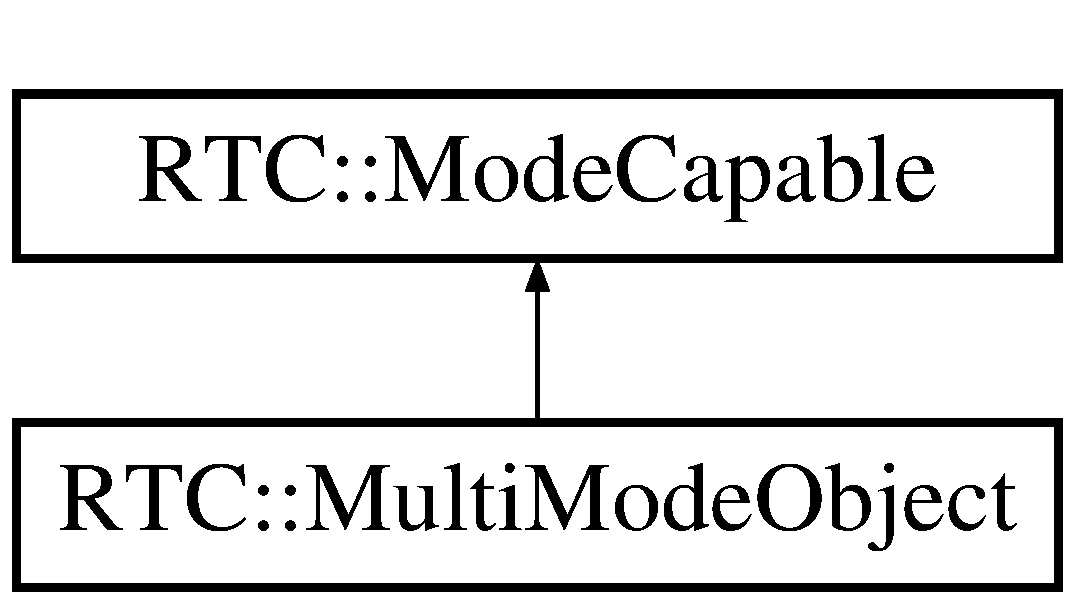
\includegraphics[height=2cm]{interfaceRTC_1_1ModeCapable}
\end{center}
\end{figure}
\subsection*{Public �᥽�å�}
\begin{CompactItemize}
\item 
{\bf Mode} {\bf get\_\-default\_\-mode} ()
\item 
{\bf Mode} {\bf get\_\-current\_\-mode} ()
\item 
{\bf Mode} {\bf get\_\-current\_\-mode\_\-in\_\-context} (in {\bf Unique\-Id} ec\_\-id)
\item 
{\bf Mode} {\bf get\_\-pending\_\-mode} ()
\item 
{\bf Mode} {\bf get\_\-pending\_\-mode\_\-in\_\-context} (in {\bf Unique\-Id} ec\_\-id)
\item 
{\bf Return\-Code\_\-t} {\bf set\_\-mode} (in {\bf Mode} new\_\-mode, in boolean immediate)
\end{CompactItemize}


\subsection{����}
Execution\-Semantics::Mode\-Capable interface. 



\subsection{�ؿ�}
\index{RTC::ModeCapable@{RTC::Mode\-Capable}!get_current_mode@{get\_\-current\_\-mode}}
\index{get_current_mode@{get\_\-current\_\-mode}!RTC::ModeCapable@{RTC::Mode\-Capable}}
\subsubsection{\setlength{\rightskip}{0pt plus 5cm}{\bf Mode} RTC::Mode\-Capable::get\_\-current\_\-mode ()}\label{interfaceRTC_1_1ModeCapable_RTC_1_1MultiModeObjecta1}


\index{RTC::ModeCapable@{RTC::Mode\-Capable}!get_current_mode_in_context@{get\_\-current\_\-mode\_\-in\_\-context}}
\index{get_current_mode_in_context@{get\_\-current\_\-mode\_\-in\_\-context}!RTC::ModeCapable@{RTC::Mode\-Capable}}
\subsubsection{\setlength{\rightskip}{0pt plus 5cm}{\bf Mode} RTC::Mode\-Capable::get\_\-current\_\-mode\_\-in\_\-context (in {\bf Unique\-Id} {\em ec\_\-id})}\label{interfaceRTC_1_1ModeCapable_RTC_1_1MultiModeObjecta2}


\index{RTC::ModeCapable@{RTC::Mode\-Capable}!get_default_mode@{get\_\-default\_\-mode}}
\index{get_default_mode@{get\_\-default\_\-mode}!RTC::ModeCapable@{RTC::Mode\-Capable}}
\subsubsection{\setlength{\rightskip}{0pt plus 5cm}{\bf Mode} RTC::Mode\-Capable::get\_\-default\_\-mode ()}\label{interfaceRTC_1_1ModeCapable_RTC_1_1MultiModeObjecta0}


\index{RTC::ModeCapable@{RTC::Mode\-Capable}!get_pending_mode@{get\_\-pending\_\-mode}}
\index{get_pending_mode@{get\_\-pending\_\-mode}!RTC::ModeCapable@{RTC::Mode\-Capable}}
\subsubsection{\setlength{\rightskip}{0pt plus 5cm}{\bf Mode} RTC::Mode\-Capable::get\_\-pending\_\-mode ()}\label{interfaceRTC_1_1ModeCapable_RTC_1_1MultiModeObjecta3}


\index{RTC::ModeCapable@{RTC::Mode\-Capable}!get_pending_mode_in_context@{get\_\-pending\_\-mode\_\-in\_\-context}}
\index{get_pending_mode_in_context@{get\_\-pending\_\-mode\_\-in\_\-context}!RTC::ModeCapable@{RTC::Mode\-Capable}}
\subsubsection{\setlength{\rightskip}{0pt plus 5cm}{\bf Mode} RTC::Mode\-Capable::get\_\-pending\_\-mode\_\-in\_\-context (in {\bf Unique\-Id} {\em ec\_\-id})}\label{interfaceRTC_1_1ModeCapable_RTC_1_1MultiModeObjecta4}


\index{RTC::ModeCapable@{RTC::Mode\-Capable}!set_mode@{set\_\-mode}}
\index{set_mode@{set\_\-mode}!RTC::ModeCapable@{RTC::Mode\-Capable}}
\subsubsection{\setlength{\rightskip}{0pt plus 5cm}{\bf Return\-Code\_\-t} RTC::Mode\-Capable::set\_\-mode (in {\bf Mode} {\em new\_\-mode}, in boolean {\em immediate})}\label{interfaceRTC_1_1ModeCapable_RTC_1_1MultiModeObjecta5}




���Υ��󥿥ե������������ϼ��Υե����뤫����������ޤ���:\begin{CompactItemize}
\item 
{\bf RTC.idl}\end{CompactItemize}

\section{���󥿥ե����� SDOPackage::Monitoring}
\label{interfaceSDOPackage_1_1Monitoring}\index{SDOPackage::Monitoring@{SDOPackage::Monitoring}}
{\tt import \char`\"{}SDOPackage.idl\char`\"{};}



���Υ��󥿥ե������������ϼ��Υե����뤫����������ޤ���:\begin{CompactItemize}
\item 
{\bf SDOPackage.idl}\end{CompactItemize}

\section{RTC::Multi\-Mode\-Component\-Action Interface Reference}
\label{interfaceRTC_1_1MultiModeComponentAction}\index{RTC::MultiModeComponentAction@{RTC::MultiModeComponentAction}}
Execution\-Semantics::Multi\-Mode\-Component\-Action interface.  


{\tt import \char`\"{}RTC.idl\char`\"{};}

Inheritance diagram for RTC::Multi\-Mode\-Component\-Action::\begin{figure}[H]
\begin{center}
\leavevmode
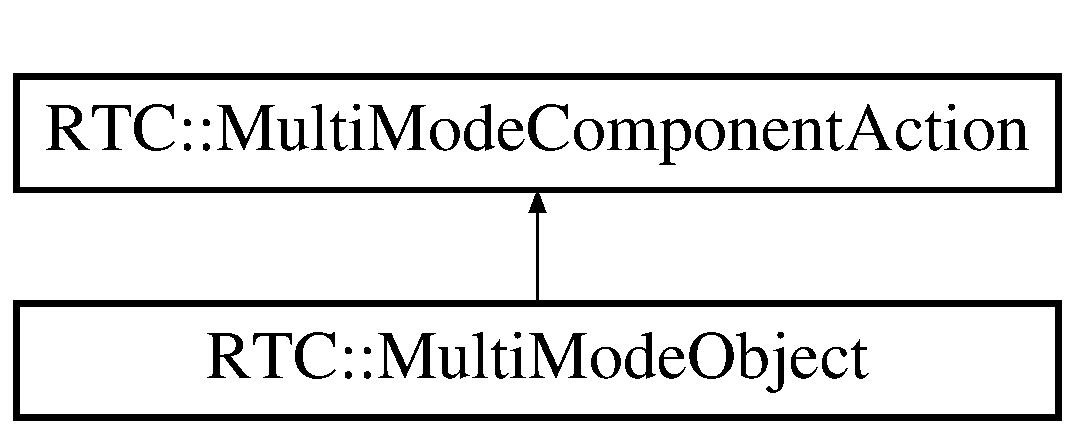
\includegraphics[height=2cm]{interfaceRTC_1_1MultiModeComponentAction}
\end{center}
\end{figure}
\subsection*{Public Member Functions}
\begin{CompactItemize}
\item 
{\bf Return\-Code\_\-t} {\bf on\_\-mode\_\-changed} (in {\bf Lightweight\-RTObject} comp, in {\bf Unique\-Id} ec\_\-id)
\end{CompactItemize}


\subsection{Detailed Description}
Execution\-Semantics::Multi\-Mode\-Component\-Action interface. 



\subsection{Member Function Documentation}
\index{RTC::MultiModeComponentAction@{RTC::Multi\-Mode\-Component\-Action}!on_mode_changed@{on\_\-mode\_\-changed}}
\index{on_mode_changed@{on\_\-mode\_\-changed}!RTC::MultiModeComponentAction@{RTC::Multi\-Mode\-Component\-Action}}
\subsubsection{\setlength{\rightskip}{0pt plus 5cm}{\bf Return\-Code\_\-t} RTC::Multi\-Mode\-Component\-Action::on\_\-mode\_\-changed (in {\bf Lightweight\-RTObject} {\em comp}, in {\bf Unique\-Id} {\em ec\_\-id})}\label{interfaceRTC_1_1MultiModeComponentAction_RTC_1_1MultiModeObjecta6}




The documentation for this interface was generated from the following file:\begin{CompactItemize}
\item 
{\bf RTC.idl}\end{CompactItemize}

\section{���󥿥ե����� RTC::Multi\-Mode\-Object}
\label{interfaceRTC_1_1MultiModeObject}\index{RTC::MultiModeObject@{RTC::MultiModeObject}}
Execution\-Semantics::Multi\-Mode\-Object interface.  


{\tt import \char`\"{}RTC.idl\char`\"{};}

RTC::Multi\-Mode\-Object���Ф���Ѿ������:\begin{figure}[H]
\begin{center}
\leavevmode
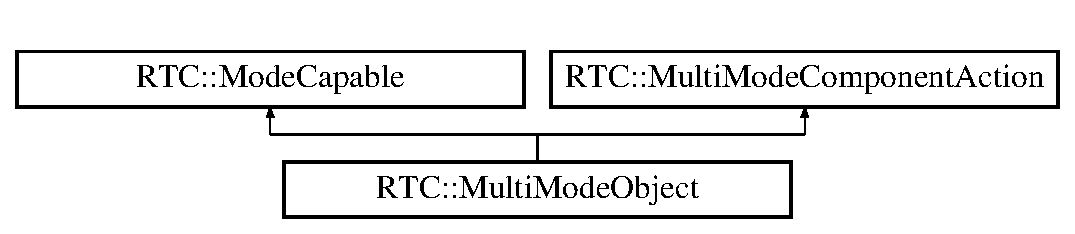
\includegraphics[height=2cm]{interfaceRTC_1_1MultiModeObject}
\end{center}
\end{figure}
\subsection*{Public �᥽�å�}
\begin{CompactItemize}
\item 
{\bf Mode} {\bf get\_\-default\_\-mode} ()
\item 
{\bf Mode} {\bf get\_\-current\_\-mode} ()
\item 
{\bf Mode} {\bf get\_\-current\_\-mode\_\-in\_\-context} (in {\bf Unique\-Id} ec\_\-id)
\item 
{\bf Mode} {\bf get\_\-pending\_\-mode} ()
\item 
{\bf Mode} {\bf get\_\-pending\_\-mode\_\-in\_\-context} (in {\bf Unique\-Id} ec\_\-id)
\item 
{\bf Return\-Code\_\-t} {\bf set\_\-mode} (in {\bf Mode} new\_\-mode, in boolean immediate)
\item 
{\bf Return\-Code\_\-t} {\bf on\_\-mode\_\-changed} (in {\bf Lightweight\-RTObject} comp, in {\bf Unique\-Id} ec\_\-id)
\end{CompactItemize}


\subsection{����}
Execution\-Semantics::Multi\-Mode\-Object interface. 



\subsection{�ؿ�}
\index{RTC::MultiModeObject@{RTC::Multi\-Mode\-Object}!get_current_mode@{get\_\-current\_\-mode}}
\index{get_current_mode@{get\_\-current\_\-mode}!RTC::MultiModeObject@{RTC::Multi\-Mode\-Object}}
\subsubsection{\setlength{\rightskip}{0pt plus 5cm}{\bf Mode} RTC::Mode\-Capable::get\_\-current\_\-mode ()\hspace{0.3cm}{\tt  [inherited]}}\label{interfaceRTC_1_1ModeCapable_RTC_1_1MultiModeObjecta1}


\index{RTC::MultiModeObject@{RTC::Multi\-Mode\-Object}!get_current_mode_in_context@{get\_\-current\_\-mode\_\-in\_\-context}}
\index{get_current_mode_in_context@{get\_\-current\_\-mode\_\-in\_\-context}!RTC::MultiModeObject@{RTC::Multi\-Mode\-Object}}
\subsubsection{\setlength{\rightskip}{0pt plus 5cm}{\bf Mode} RTC::Mode\-Capable::get\_\-current\_\-mode\_\-in\_\-context (in {\bf Unique\-Id} {\em ec\_\-id})\hspace{0.3cm}{\tt  [inherited]}}\label{interfaceRTC_1_1ModeCapable_RTC_1_1MultiModeObjecta2}


\index{RTC::MultiModeObject@{RTC::Multi\-Mode\-Object}!get_default_mode@{get\_\-default\_\-mode}}
\index{get_default_mode@{get\_\-default\_\-mode}!RTC::MultiModeObject@{RTC::Multi\-Mode\-Object}}
\subsubsection{\setlength{\rightskip}{0pt plus 5cm}{\bf Mode} RTC::Mode\-Capable::get\_\-default\_\-mode ()\hspace{0.3cm}{\tt  [inherited]}}\label{interfaceRTC_1_1ModeCapable_RTC_1_1MultiModeObjecta0}


\index{RTC::MultiModeObject@{RTC::Multi\-Mode\-Object}!get_pending_mode@{get\_\-pending\_\-mode}}
\index{get_pending_mode@{get\_\-pending\_\-mode}!RTC::MultiModeObject@{RTC::Multi\-Mode\-Object}}
\subsubsection{\setlength{\rightskip}{0pt plus 5cm}{\bf Mode} RTC::Mode\-Capable::get\_\-pending\_\-mode ()\hspace{0.3cm}{\tt  [inherited]}}\label{interfaceRTC_1_1ModeCapable_RTC_1_1MultiModeObjecta3}


\index{RTC::MultiModeObject@{RTC::Multi\-Mode\-Object}!get_pending_mode_in_context@{get\_\-pending\_\-mode\_\-in\_\-context}}
\index{get_pending_mode_in_context@{get\_\-pending\_\-mode\_\-in\_\-context}!RTC::MultiModeObject@{RTC::Multi\-Mode\-Object}}
\subsubsection{\setlength{\rightskip}{0pt plus 5cm}{\bf Mode} RTC::Mode\-Capable::get\_\-pending\_\-mode\_\-in\_\-context (in {\bf Unique\-Id} {\em ec\_\-id})\hspace{0.3cm}{\tt  [inherited]}}\label{interfaceRTC_1_1ModeCapable_RTC_1_1MultiModeObjecta4}


\index{RTC::MultiModeObject@{RTC::Multi\-Mode\-Object}!on_mode_changed@{on\_\-mode\_\-changed}}
\index{on_mode_changed@{on\_\-mode\_\-changed}!RTC::MultiModeObject@{RTC::Multi\-Mode\-Object}}
\subsubsection{\setlength{\rightskip}{0pt plus 5cm}{\bf Return\-Code\_\-t} RTC::Multi\-Mode\-Component\-Action::on\_\-mode\_\-changed (in {\bf Lightweight\-RTObject} {\em comp}, in {\bf Unique\-Id} {\em ec\_\-id})\hspace{0.3cm}{\tt  [inherited]}}\label{interfaceRTC_1_1MultiModeComponentAction_RTC_1_1MultiModeObjecta6}


\index{RTC::MultiModeObject@{RTC::Multi\-Mode\-Object}!set_mode@{set\_\-mode}}
\index{set_mode@{set\_\-mode}!RTC::MultiModeObject@{RTC::Multi\-Mode\-Object}}
\subsubsection{\setlength{\rightskip}{0pt plus 5cm}{\bf Return\-Code\_\-t} RTC::Mode\-Capable::set\_\-mode (in {\bf Mode} {\em new\_\-mode}, in boolean {\em immediate})\hspace{0.3cm}{\tt  [inherited]}}\label{interfaceRTC_1_1ModeCapable_RTC_1_1MultiModeObjecta5}




���Υ��󥿥ե������������ϼ��Υե����뤫����������ޤ���:\begin{CompactItemize}
\item 
{\bf RTC.idl}\end{CompactItemize}

\section{SDOPackage::Name\-Value Struct Reference}
\label{structSDOPackage_1_1NameValue}\index{SDOPackage::NameValue@{SDOPackage::NameValue}}
{\tt import \char`\"{}SDOPackage.idl\char`\"{};}

\subsection*{Public Attributes}
\begin{CompactItemize}
\item 
string {\bf name}
\item 
any {\bf value}
\end{CompactItemize}


\subsection{Member Data Documentation}
\index{SDOPackage::NameValue@{SDOPackage::Name\-Value}!name@{name}}
\index{name@{name}!SDOPackage::NameValue@{SDOPackage::Name\-Value}}
\subsubsection{\setlength{\rightskip}{0pt plus 5cm}string {\bf SDOPackage::Name\-Value::name}}\label{structSDOPackage_1_1NameValue_SDOPackage_1_1NameValueo0}


\index{SDOPackage::NameValue@{SDOPackage::Name\-Value}!value@{value}}
\index{value@{value}!SDOPackage::NameValue@{SDOPackage::Name\-Value}}
\subsubsection{\setlength{\rightskip}{0pt plus 5cm}any {\bf SDOPackage::Name\-Value::value}}\label{structSDOPackage_1_1NameValue_SDOPackage_1_1NameValueo1}




The documentation for this struct was generated from the following file:\begin{CompactItemize}
\item 
{\bf SDOPackage.idl}\end{CompactItemize}

\section{������ SDOPackage::Numeric}
\label{unionSDOPackage_1_1Numeric}\index{SDOPackage::Numeric@{SDOPackage::Numeric}}
{\tt import \char`\"{}SDOPackage.idl\char`\"{};}

\subsection*{Public �ѿ�}
\begin{CompactItemize}
\item 
short {\bf short\_\-value}
\item 
long {\bf long\_\-value}
\item 
float {\bf float\_\-value}
\item 
double {\bf double\_\-value}
\end{CompactItemize}


\subsection{�ѿ�}
\index{SDOPackage::Numeric@{SDOPackage::Numeric}!double_value@{double\_\-value}}
\index{double_value@{double\_\-value}!SDOPackage::Numeric@{SDOPackage::Numeric}}
\subsubsection{\setlength{\rightskip}{0pt plus 5cm}double {\bf SDOPackage::Numeric::double\_\-value}}\label{unionSDOPackage_1_1Numeric_SDOPackage_1_1Numerico3}


\index{SDOPackage::Numeric@{SDOPackage::Numeric}!float_value@{float\_\-value}}
\index{float_value@{float\_\-value}!SDOPackage::Numeric@{SDOPackage::Numeric}}
\subsubsection{\setlength{\rightskip}{0pt plus 5cm}float {\bf SDOPackage::Numeric::float\_\-value}}\label{unionSDOPackage_1_1Numeric_SDOPackage_1_1Numerico2}


\index{SDOPackage::Numeric@{SDOPackage::Numeric}!long_value@{long\_\-value}}
\index{long_value@{long\_\-value}!SDOPackage::Numeric@{SDOPackage::Numeric}}
\subsubsection{\setlength{\rightskip}{0pt plus 5cm}long {\bf SDOPackage::Numeric::long\_\-value}}\label{unionSDOPackage_1_1Numeric_SDOPackage_1_1Numerico1}


\index{SDOPackage::Numeric@{SDOPackage::Numeric}!short_value@{short\_\-value}}
\index{short_value@{short\_\-value}!SDOPackage::Numeric@{SDOPackage::Numeric}}
\subsubsection{\setlength{\rightskip}{0pt plus 5cm}short {\bf SDOPackage::Numeric::short\_\-value}}\label{unionSDOPackage_1_1Numeric_SDOPackage_1_1Numerico0}




���ζ����Τ������ϼ��Υե����뤫����������ޤ���:\begin{CompactItemize}
\item 
{\bf SDOPackage.idl}\end{CompactItemize}

\section{���󥿥ե����� SDOPackage::Organization}
\label{interfaceSDOPackage_1_1Organization}\index{SDOPackage::Organization@{SDOPackage::Organization}}
{\tt import \char`\"{}SDOPackage.idl\char`\"{};}

\subsection*{Public �᥽�å�}
\begin{CompactItemize}
\item 
{\bf Unique\-Identifier} {\bf get\_\-organization\_\-id} ()  raises (Invalid\-Parameter, Not\-Available, Internal\-Error)
\item 
{\bf Organization\-Property} {\bf get\_\-organization\_\-property} ()  raises (Not\-Available, Internal\-Error)
\item 
any {\bf get\_\-organization\_\-property\_\-value} (in string name)  raises (Invalid\-Parameter, Not\-Available, Internal\-Error)
\item 
boolean {\bf set\_\-organization\_\-property} (in {\bf Organization\-Property} organization\_\-property)  raises (Invalid\-Parameter, Not\-Available, Internal\-Error)
\item 
boolean {\bf set\_\-organization\_\-property\_\-value} (in string name, in any value)  raises (Invalid\-Parameter, Not\-Available, Internal\-Error)
\item 
boolean {\bf remove\_\-organization\_\-property} (in string name)  raises (Invalid\-Parameter, Not\-Available, Internal\-Error)
\item 
{\bf SDOSystem\-Element} {\bf get\_\-owner} ()  raises (Not\-Available, Internal\-Error)
\item 
boolean {\bf set\_\-owner} (in {\bf SDOSystem\-Element} sdo)  raises (Invalid\-Parameter, Not\-Available, Internal\-Error)
\item 
{\bf SDOList} {\bf get\_\-members} ()  raises (Not\-Available, Internal\-Error)
\item 
boolean {\bf set\_\-members} (in {\bf SDOList} sdos)  raises (Invalid\-Parameter, Not\-Available, Internal\-Error)
\item 
boolean {\bf add\_\-members} (in {\bf SDOList} sdo\_\-list)  raises (Invalid\-Parameter, Not\-Available, Internal\-Error)
\item 
boolean {\bf remove\_\-member} (in {\bf Unique\-Identifier} id)  raises (Invalid\-Parameter, Not\-Available, Internal\-Error)
\item 
{\bf Dependency\-Type} {\bf get\_\-dependency} ()  raises (Not\-Available, Internal\-Error)
\item 
boolean {\bf set\_\-dependency} (in {\bf Dependency\-Type} dependency)  raises (Not\-Available, Internal\-Error)
\end{CompactItemize}


\subsection{�ؿ�}
\index{SDOPackage::Organization@{SDOPackage::Organization}!add_members@{add\_\-members}}
\index{add_members@{add\_\-members}!SDOPackage::Organization@{SDOPackage::Organization}}
\subsubsection{\setlength{\rightskip}{0pt plus 5cm}boolean SDOPackage::Organization::add\_\-members (in {\bf SDOList} {\em sdo\_\-list})  raises (Invalid\-Parameter, Not\-Available, Internal\-Error)}\label{interfaceSDOPackage_1_1Organization_SDOPackage_1_1Organizationa10}


\index{SDOPackage::Organization@{SDOPackage::Organization}!get_dependency@{get\_\-dependency}}
\index{get_dependency@{get\_\-dependency}!SDOPackage::Organization@{SDOPackage::Organization}}
\subsubsection{\setlength{\rightskip}{0pt plus 5cm}{\bf Dependency\-Type} SDOPackage::Organization::get\_\-dependency ()  raises (Not\-Available, Internal\-Error)}\label{interfaceSDOPackage_1_1Organization_SDOPackage_1_1Organizationa12}


\index{SDOPackage::Organization@{SDOPackage::Organization}!get_members@{get\_\-members}}
\index{get_members@{get\_\-members}!SDOPackage::Organization@{SDOPackage::Organization}}
\subsubsection{\setlength{\rightskip}{0pt plus 5cm}{\bf SDOList} SDOPackage::Organization::get\_\-members ()  raises (Not\-Available, Internal\-Error)}\label{interfaceSDOPackage_1_1Organization_SDOPackage_1_1Organizationa8}


\index{SDOPackage::Organization@{SDOPackage::Organization}!get_organization_id@{get\_\-organization\_\-id}}
\index{get_organization_id@{get\_\-organization\_\-id}!SDOPackage::Organization@{SDOPackage::Organization}}
\subsubsection{\setlength{\rightskip}{0pt plus 5cm}{\bf Unique\-Identifier} SDOPackage::Organization::get\_\-organization\_\-id ()  raises (Invalid\-Parameter, Not\-Available, Internal\-Error)}\label{interfaceSDOPackage_1_1Organization_SDOPackage_1_1Organizationa0}


\index{SDOPackage::Organization@{SDOPackage::Organization}!get_organization_property@{get\_\-organization\_\-property}}
\index{get_organization_property@{get\_\-organization\_\-property}!SDOPackage::Organization@{SDOPackage::Organization}}
\subsubsection{\setlength{\rightskip}{0pt plus 5cm}{\bf Organization\-Property} SDOPackage::Organization::get\_\-organization\_\-property ()  raises (Not\-Available, Internal\-Error)}\label{interfaceSDOPackage_1_1Organization_SDOPackage_1_1Organizationa1}


\index{SDOPackage::Organization@{SDOPackage::Organization}!get_organization_property_value@{get\_\-organization\_\-property\_\-value}}
\index{get_organization_property_value@{get\_\-organization\_\-property\_\-value}!SDOPackage::Organization@{SDOPackage::Organization}}
\subsubsection{\setlength{\rightskip}{0pt plus 5cm}any SDOPackage::Organization::get\_\-organization\_\-property\_\-value (in string {\em name})  raises (Invalid\-Parameter, Not\-Available, Internal\-Error)}\label{interfaceSDOPackage_1_1Organization_SDOPackage_1_1Organizationa2}


\index{SDOPackage::Organization@{SDOPackage::Organization}!get_owner@{get\_\-owner}}
\index{get_owner@{get\_\-owner}!SDOPackage::Organization@{SDOPackage::Organization}}
\subsubsection{\setlength{\rightskip}{0pt plus 5cm}{\bf SDOSystem\-Element} SDOPackage::Organization::get\_\-owner ()  raises (Not\-Available, Internal\-Error)}\label{interfaceSDOPackage_1_1Organization_SDOPackage_1_1Organizationa6}


\index{SDOPackage::Organization@{SDOPackage::Organization}!remove_member@{remove\_\-member}}
\index{remove_member@{remove\_\-member}!SDOPackage::Organization@{SDOPackage::Organization}}
\subsubsection{\setlength{\rightskip}{0pt plus 5cm}boolean SDOPackage::Organization::remove\_\-member (in {\bf Unique\-Identifier} {\em id})  raises (Invalid\-Parameter, Not\-Available, Internal\-Error)}\label{interfaceSDOPackage_1_1Organization_SDOPackage_1_1Organizationa11}


\index{SDOPackage::Organization@{SDOPackage::Organization}!remove_organization_property@{remove\_\-organization\_\-property}}
\index{remove_organization_property@{remove\_\-organization\_\-property}!SDOPackage::Organization@{SDOPackage::Organization}}
\subsubsection{\setlength{\rightskip}{0pt plus 5cm}boolean SDOPackage::Organization::remove\_\-organization\_\-property (in string {\em name})  raises (Invalid\-Parameter, Not\-Available, Internal\-Error)}\label{interfaceSDOPackage_1_1Organization_SDOPackage_1_1Organizationa5}


\index{SDOPackage::Organization@{SDOPackage::Organization}!set_dependency@{set\_\-dependency}}
\index{set_dependency@{set\_\-dependency}!SDOPackage::Organization@{SDOPackage::Organization}}
\subsubsection{\setlength{\rightskip}{0pt plus 5cm}boolean SDOPackage::Organization::set\_\-dependency (in {\bf Dependency\-Type} {\em dependency})  raises (Not\-Available, Internal\-Error)}\label{interfaceSDOPackage_1_1Organization_SDOPackage_1_1Organizationa13}


\index{SDOPackage::Organization@{SDOPackage::Organization}!set_members@{set\_\-members}}
\index{set_members@{set\_\-members}!SDOPackage::Organization@{SDOPackage::Organization}}
\subsubsection{\setlength{\rightskip}{0pt plus 5cm}boolean SDOPackage::Organization::set\_\-members (in {\bf SDOList} {\em sdos})  raises (Invalid\-Parameter, Not\-Available, Internal\-Error)}\label{interfaceSDOPackage_1_1Organization_SDOPackage_1_1Organizationa9}


\index{SDOPackage::Organization@{SDOPackage::Organization}!set_organization_property@{set\_\-organization\_\-property}}
\index{set_organization_property@{set\_\-organization\_\-property}!SDOPackage::Organization@{SDOPackage::Organization}}
\subsubsection{\setlength{\rightskip}{0pt plus 5cm}boolean SDOPackage::Organization::set\_\-organization\_\-property (in {\bf Organization\-Property} {\em organization\_\-property})  raises (Invalid\-Parameter, Not\-Available, Internal\-Error)}\label{interfaceSDOPackage_1_1Organization_SDOPackage_1_1Organizationa3}


\index{SDOPackage::Organization@{SDOPackage::Organization}!set_organization_property_value@{set\_\-organization\_\-property\_\-value}}
\index{set_organization_property_value@{set\_\-organization\_\-property\_\-value}!SDOPackage::Organization@{SDOPackage::Organization}}
\subsubsection{\setlength{\rightskip}{0pt plus 5cm}boolean SDOPackage::Organization::set\_\-organization\_\-property\_\-value (in string {\em name}, in any {\em value})  raises (Invalid\-Parameter, Not\-Available, Internal\-Error)}\label{interfaceSDOPackage_1_1Organization_SDOPackage_1_1Organizationa4}


\index{SDOPackage::Organization@{SDOPackage::Organization}!set_owner@{set\_\-owner}}
\index{set_owner@{set\_\-owner}!SDOPackage::Organization@{SDOPackage::Organization}}
\subsubsection{\setlength{\rightskip}{0pt plus 5cm}boolean SDOPackage::Organization::set\_\-owner (in {\bf SDOSystem\-Element} {\em sdo})  raises (Invalid\-Parameter, Not\-Available, Internal\-Error)}\label{interfaceSDOPackage_1_1Organization_SDOPackage_1_1Organizationa7}




���Υ��󥿥ե������������ϼ��Υե����뤫����������ޤ���:\begin{CompactItemize}
\item 
{\bf SDOPackage.idl}\end{CompactItemize}

\section{��¤�� SDOPackage::Organization\-Property}
\label{structSDOPackage_1_1OrganizationProperty}\index{SDOPackage::OrganizationProperty@{SDOPackage::OrganizationProperty}}
{\tt import \char`\"{}SDOPackage.idl\char`\"{};}

\subsection*{Public �ѿ�}
\begin{CompactItemize}
\item 
{\bf NVList} {\bf properties}
\end{CompactItemize}


\subsection{�ѿ�}
\index{SDOPackage::OrganizationProperty@{SDOPackage::Organization\-Property}!properties@{properties}}
\index{properties@{properties}!SDOPackage::OrganizationProperty@{SDOPackage::Organization\-Property}}
\subsubsection{\setlength{\rightskip}{0pt plus 5cm}{\bf NVList} {\bf SDOPackage::Organization\-Property::properties}}\label{structSDOPackage_1_1OrganizationProperty_SDOPackage_1_1OrganizationPropertyo0}




���ι�¤�Τ������ϼ��Υե����뤫����������ޤ���:\begin{CompactItemize}
\item 
{\bf SDOPackage.idl}\end{CompactItemize}

\section{���󥿥ե����� RTC::Out\-Port\-Any}
\label{interfaceRTC_1_1OutPortAny}\index{RTC::OutPortAny@{RTC::OutPortAny}}
{\tt import \char`\"{}Data\-Port.idl\char`\"{};}

\subsection*{Public �᥽�å�}
\begin{CompactItemize}
\item 
any {\bf get} ()
\end{CompactItemize}


\subsection{�ؿ�}
\index{RTC::OutPortAny@{RTC::Out\-Port\-Any}!get@{get}}
\index{get@{get}!RTC::OutPortAny@{RTC::Out\-Port\-Any}}
\subsubsection{\setlength{\rightskip}{0pt plus 5cm}any RTC::Out\-Port\-Any::get ()}\label{interfaceRTC_1_1OutPortAny_RTC_1_1OutPortAnya0}




���Υ��󥿥ե������������ϼ��Υե����뤫����������ޤ���:\begin{CompactItemize}
\item 
{\bf Data\-Port.idl}\end{CompactItemize}

\section{SDOPackage::Parameter Struct Reference}
\label{structSDOPackage_1_1Parameter}\index{SDOPackage::Parameter@{SDOPackage::Parameter}}
{\tt import \char`\"{}SDOPackage.idl\char`\"{};}

\subsection*{Public Attributes}
\begin{CompactItemize}
\item 
string {\bf name}
\item 
Type\-Code {\bf type}
\item 
{\bf Allowed\-Values} {\bf allowed\_\-values}
\end{CompactItemize}


\subsection{Member Data Documentation}
\index{SDOPackage::Parameter@{SDOPackage::Parameter}!allowed_values@{allowed\_\-values}}
\index{allowed_values@{allowed\_\-values}!SDOPackage::Parameter@{SDOPackage::Parameter}}
\subsubsection{\setlength{\rightskip}{0pt plus 5cm}{\bf Allowed\-Values} {\bf SDOPackage::Parameter::allowed\_\-values}}\label{structSDOPackage_1_1Parameter_SDOPackage_1_1Parametero2}


\index{SDOPackage::Parameter@{SDOPackage::Parameter}!name@{name}}
\index{name@{name}!SDOPackage::Parameter@{SDOPackage::Parameter}}
\subsubsection{\setlength{\rightskip}{0pt plus 5cm}string {\bf SDOPackage::Parameter::name}}\label{structSDOPackage_1_1Parameter_SDOPackage_1_1Parametero0}


\index{SDOPackage::Parameter@{SDOPackage::Parameter}!type@{type}}
\index{type@{type}!SDOPackage::Parameter@{SDOPackage::Parameter}}
\subsubsection{\setlength{\rightskip}{0pt plus 5cm}Type\-Code {\bf SDOPackage::Parameter::type}}\label{structSDOPackage_1_1Parameter_SDOPackage_1_1Parametero1}




The documentation for this struct was generated from the following file:\begin{CompactItemize}
\item 
{\bf SDOPackage.idl}\end{CompactItemize}

\section{RTC::Port Interface Reference}
\label{interfaceRTC_1_1Port}\index{RTC::Port@{RTC::Port}}
Introspection::Port interface.  


{\tt import \char`\"{}RTC.idl\char`\"{};}

Inheritance diagram for RTC::Port::\begin{figure}[H]
\begin{center}
\leavevmode
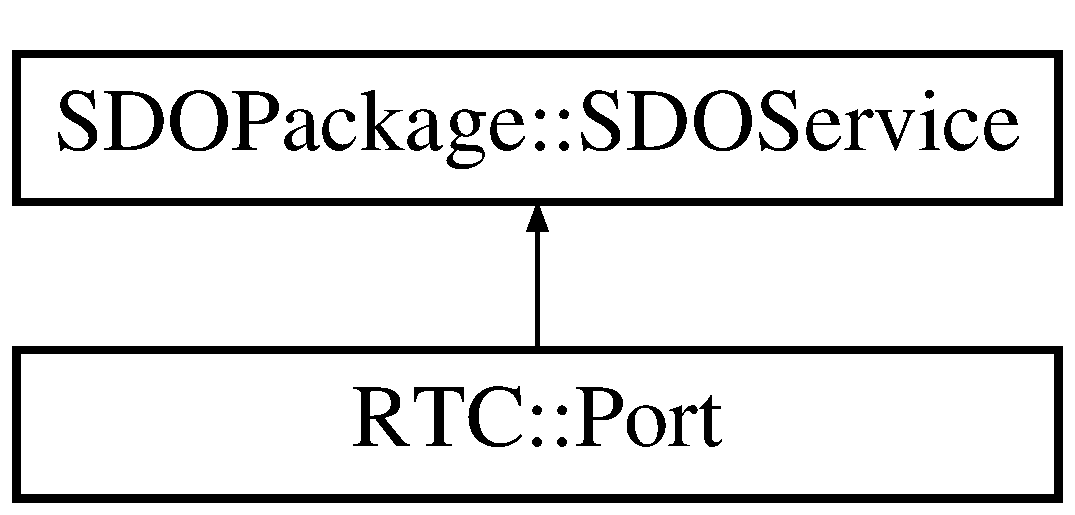
\includegraphics[height=2cm]{interfaceRTC_1_1Port}
\end{center}
\end{figure}
\subsection*{Public Member Functions}
\begin{CompactItemize}
\item 
{\bf Port\-Profile} {\bf get\_\-port\_\-profile} ()
\item 
{\bf Connector\-Profile\-List} {\bf get\_\-connector\_\-profiles} ()
\item 
{\bf Connector\-Profile} {\bf get\_\-connector\_\-profile} (in {\bf Unique\-Identifier} connector\_\-id)
\item 
{\bf Return\-Code\_\-t} {\bf connect} (inout {\bf Connector\-Profile} connector\_\-profile)
\item 
{\bf Return\-Code\_\-t} {\bf notify\_\-connect} (inout {\bf Connector\-Profile} connector\_\-profile)
\item 
{\bf Return\-Code\_\-t} {\bf disconnect} (in {\bf Unique\-Identifier} connector\_\-id)
\item 
{\bf Return\-Code\_\-t} {\bf notify\_\-disconnect} (in {\bf Unique\-Identifier} connector\_\-id)
\item 
{\bf Return\-Code\_\-t} {\bf disconnect\_\-all} ()
\end{CompactItemize}


\subsection{Detailed Description}
Introspection::Port interface. 



\subsection{Member Function Documentation}
\index{RTC::Port@{RTC::Port}!connect@{connect}}
\index{connect@{connect}!RTC::Port@{RTC::Port}}
\subsubsection{\setlength{\rightskip}{0pt plus 5cm}{\bf Return\-Code\_\-t} RTC::Port::connect (inout {\bf Connector\-Profile} {\em connector\_\-profile})}\label{interfaceRTC_1_1Port_RTC_1_1Porta3}


\index{RTC::Port@{RTC::Port}!disconnect@{disconnect}}
\index{disconnect@{disconnect}!RTC::Port@{RTC::Port}}
\subsubsection{\setlength{\rightskip}{0pt plus 5cm}{\bf Return\-Code\_\-t} RTC::Port::disconnect (in {\bf Unique\-Identifier} {\em connector\_\-id})}\label{interfaceRTC_1_1Port_RTC_1_1Porta5}


\index{RTC::Port@{RTC::Port}!disconnect_all@{disconnect\_\-all}}
\index{disconnect_all@{disconnect\_\-all}!RTC::Port@{RTC::Port}}
\subsubsection{\setlength{\rightskip}{0pt plus 5cm}{\bf Return\-Code\_\-t} RTC::Port::disconnect\_\-all ()}\label{interfaceRTC_1_1Port_RTC_1_1Porta7}


\index{RTC::Port@{RTC::Port}!get_connector_profile@{get\_\-connector\_\-profile}}
\index{get_connector_profile@{get\_\-connector\_\-profile}!RTC::Port@{RTC::Port}}
\subsubsection{\setlength{\rightskip}{0pt plus 5cm}{\bf Connector\-Profile} RTC::Port::get\_\-connector\_\-profile (in {\bf Unique\-Identifier} {\em connector\_\-id})}\label{interfaceRTC_1_1Port_RTC_1_1Porta2}


\index{RTC::Port@{RTC::Port}!get_connector_profiles@{get\_\-connector\_\-profiles}}
\index{get_connector_profiles@{get\_\-connector\_\-profiles}!RTC::Port@{RTC::Port}}
\subsubsection{\setlength{\rightskip}{0pt plus 5cm}{\bf Connector\-Profile\-List} RTC::Port::get\_\-connector\_\-profiles ()}\label{interfaceRTC_1_1Port_RTC_1_1Porta1}


\index{RTC::Port@{RTC::Port}!get_port_profile@{get\_\-port\_\-profile}}
\index{get_port_profile@{get\_\-port\_\-profile}!RTC::Port@{RTC::Port}}
\subsubsection{\setlength{\rightskip}{0pt plus 5cm}{\bf Port\-Profile} RTC::Port::get\_\-port\_\-profile ()}\label{interfaceRTC_1_1Port_RTC_1_1Porta0}


\index{RTC::Port@{RTC::Port}!notify_connect@{notify\_\-connect}}
\index{notify_connect@{notify\_\-connect}!RTC::Port@{RTC::Port}}
\subsubsection{\setlength{\rightskip}{0pt plus 5cm}{\bf Return\-Code\_\-t} RTC::Port::notify\_\-connect (inout {\bf Connector\-Profile} {\em connector\_\-profile})}\label{interfaceRTC_1_1Port_RTC_1_1Porta4}


\index{RTC::Port@{RTC::Port}!notify_disconnect@{notify\_\-disconnect}}
\index{notify_disconnect@{notify\_\-disconnect}!RTC::Port@{RTC::Port}}
\subsubsection{\setlength{\rightskip}{0pt plus 5cm}{\bf Return\-Code\_\-t} RTC::Port::notify\_\-disconnect (in {\bf Unique\-Identifier} {\em connector\_\-id})}\label{interfaceRTC_1_1Port_RTC_1_1Porta6}




The documentation for this interface was generated from the following file:\begin{CompactItemize}
\item 
{\bf RTC.idl}\end{CompactItemize}

\section{RTC::Port\-Interface\-Profile Struct Reference}
\label{structRTC_1_1PortInterfaceProfile}\index{RTC::PortInterfaceProfile@{RTC::PortInterfaceProfile}}
Introspection::Port\-Interface\-Profile structure.  


{\tt import \char`\"{}RTC.idl\char`\"{};}

\subsection*{Public Attributes}
\begin{CompactItemize}
\item 
string {\bf instance\_\-name}
\item 
string {\bf type\_\-name}
\item 
{\bf Port\-Interface\-Polarity} {\bf polarity}
\end{CompactItemize}


\subsection{Detailed Description}
Introspection::Port\-Interface\-Profile structure. 



\subsection{Member Data Documentation}
\index{RTC::PortInterfaceProfile@{RTC::Port\-Interface\-Profile}!instance_name@{instance\_\-name}}
\index{instance_name@{instance\_\-name}!RTC::PortInterfaceProfile@{RTC::Port\-Interface\-Profile}}
\subsubsection{\setlength{\rightskip}{0pt plus 5cm}string {\bf RTC::Port\-Interface\-Profile::instance\_\-name}}\label{structRTC_1_1PortInterfaceProfile_RTC_1_1PortInterfaceProfileo0}


\index{RTC::PortInterfaceProfile@{RTC::Port\-Interface\-Profile}!polarity@{polarity}}
\index{polarity@{polarity}!RTC::PortInterfaceProfile@{RTC::Port\-Interface\-Profile}}
\subsubsection{\setlength{\rightskip}{0pt plus 5cm}{\bf Port\-Interface\-Polarity} {\bf RTC::Port\-Interface\-Profile::polarity}}\label{structRTC_1_1PortInterfaceProfile_RTC_1_1PortInterfaceProfileo2}


\index{RTC::PortInterfaceProfile@{RTC::Port\-Interface\-Profile}!type_name@{type\_\-name}}
\index{type_name@{type\_\-name}!RTC::PortInterfaceProfile@{RTC::Port\-Interface\-Profile}}
\subsubsection{\setlength{\rightskip}{0pt plus 5cm}string {\bf RTC::Port\-Interface\-Profile::type\_\-name}}\label{structRTC_1_1PortInterfaceProfile_RTC_1_1PortInterfaceProfileo1}




The documentation for this struct was generated from the following file:\begin{CompactItemize}
\item 
{\bf RTC.idl}\end{CompactItemize}

\section{RTC::Port\-Profile Struct Reference}
\label{structRTC_1_1PortProfile}\index{RTC::PortProfile@{RTC::PortProfile}}
Introspection::Port\-Profile structure.  


{\tt import \char`\"{}RTC.idl\char`\"{};}

\subsection*{Public Attributes}
\begin{CompactItemize}
\item 
string {\bf name}
\item 
{\bf Port\-Interface\-Profile\-List} {\bf interfaces}
\item 
{\bf Port} {\bf port\_\-ref}
\item 
{\bf Connector\-Profile\-List} {\bf connector\_\-profiles}
\item 
{\bf RTObject} {\bf owner}
\item 
{\bf NVList} {\bf properties}
\end{CompactItemize}


\subsection{Detailed Description}
Introspection::Port\-Profile structure. 



\subsection{Member Data Documentation}
\index{RTC::PortProfile@{RTC::Port\-Profile}!connector_profiles@{connector\_\-profiles}}
\index{connector_profiles@{connector\_\-profiles}!RTC::PortProfile@{RTC::Port\-Profile}}
\subsubsection{\setlength{\rightskip}{0pt plus 5cm}{\bf Connector\-Profile\-List} {\bf RTC::Port\-Profile::connector\_\-profiles}}\label{structRTC_1_1PortProfile_RTC_1_1PortProfileo3}


\index{RTC::PortProfile@{RTC::Port\-Profile}!interfaces@{interfaces}}
\index{interfaces@{interfaces}!RTC::PortProfile@{RTC::Port\-Profile}}
\subsubsection{\setlength{\rightskip}{0pt plus 5cm}{\bf Port\-Interface\-Profile\-List} {\bf RTC::Port\-Profile::interfaces}}\label{structRTC_1_1PortProfile_RTC_1_1PortProfileo1}


\index{RTC::PortProfile@{RTC::Port\-Profile}!name@{name}}
\index{name@{name}!RTC::PortProfile@{RTC::Port\-Profile}}
\subsubsection{\setlength{\rightskip}{0pt plus 5cm}string {\bf RTC::Port\-Profile::name}}\label{structRTC_1_1PortProfile_RTC_1_1PortProfileo0}


\index{RTC::PortProfile@{RTC::Port\-Profile}!owner@{owner}}
\index{owner@{owner}!RTC::PortProfile@{RTC::Port\-Profile}}
\subsubsection{\setlength{\rightskip}{0pt plus 5cm}{\bf RTObject} {\bf RTC::Port\-Profile::owner}}\label{structRTC_1_1PortProfile_RTC_1_1PortProfileo4}


\index{RTC::PortProfile@{RTC::Port\-Profile}!port_ref@{port\_\-ref}}
\index{port_ref@{port\_\-ref}!RTC::PortProfile@{RTC::Port\-Profile}}
\subsubsection{\setlength{\rightskip}{0pt plus 5cm}{\bf Port} {\bf RTC::Port\-Profile::port\_\-ref}}\label{structRTC_1_1PortProfile_RTC_1_1PortProfileo2}


\index{RTC::PortProfile@{RTC::Port\-Profile}!properties@{properties}}
\index{properties@{properties}!RTC::PortProfile@{RTC::Port\-Profile}}
\subsubsection{\setlength{\rightskip}{0pt plus 5cm}{\bf NVList} {\bf RTC::Port\-Profile::properties}}\label{structRTC_1_1PortProfile_RTC_1_1PortProfileo5}




The documentation for this struct was generated from the following file:\begin{CompactItemize}
\item 
{\bf RTC.idl}\end{CompactItemize}

\section{SDOPackage::Range\-Type Struct Reference}
\label{structSDOPackage_1_1RangeType}\index{SDOPackage::RangeType@{SDOPackage::RangeType}}
{\tt import \char`\"{}SDOPackage.idl\char`\"{};}

\subsection*{Public Attributes}
\begin{CompactItemize}
\item 
{\bf Numeric} {\bf min}
\item 
{\bf Numeric} {\bf max}
\item 
boolean {\bf min\_\-inclusive}
\item 
boolean {\bf max\_\-inclusive}
\end{CompactItemize}


\subsection{Member Data Documentation}
\index{SDOPackage::RangeType@{SDOPackage::Range\-Type}!max@{max}}
\index{max@{max}!SDOPackage::RangeType@{SDOPackage::Range\-Type}}
\subsubsection{\setlength{\rightskip}{0pt plus 5cm}{\bf Numeric} {\bf SDOPackage::Range\-Type::max}}\label{structSDOPackage_1_1RangeType_SDOPackage_1_1RangeTypeo1}


\index{SDOPackage::RangeType@{SDOPackage::Range\-Type}!max_inclusive@{max\_\-inclusive}}
\index{max_inclusive@{max\_\-inclusive}!SDOPackage::RangeType@{SDOPackage::Range\-Type}}
\subsubsection{\setlength{\rightskip}{0pt plus 5cm}boolean {\bf SDOPackage::Range\-Type::max\_\-inclusive}}\label{structSDOPackage_1_1RangeType_SDOPackage_1_1RangeTypeo3}


\index{SDOPackage::RangeType@{SDOPackage::Range\-Type}!min@{min}}
\index{min@{min}!SDOPackage::RangeType@{SDOPackage::Range\-Type}}
\subsubsection{\setlength{\rightskip}{0pt plus 5cm}{\bf Numeric} {\bf SDOPackage::Range\-Type::min}}\label{structSDOPackage_1_1RangeType_SDOPackage_1_1RangeTypeo0}


\index{SDOPackage::RangeType@{SDOPackage::Range\-Type}!min_inclusive@{min\_\-inclusive}}
\index{min_inclusive@{min\_\-inclusive}!SDOPackage::RangeType@{SDOPackage::Range\-Type}}
\subsubsection{\setlength{\rightskip}{0pt plus 5cm}boolean {\bf SDOPackage::Range\-Type::min\_\-inclusive}}\label{structSDOPackage_1_1RangeType_SDOPackage_1_1RangeTypeo2}




The documentation for this struct was generated from the following file:\begin{CompactItemize}
\item 
{\bf SDOPackage.idl}\end{CompactItemize}

\section{���󥿥ե����� RTC::RTObject}
\label{interfaceRTC_1_1RTObject}\index{RTC::RTObject@{RTC::RTObject}}
Introspection::RTObject interface.  


{\tt import \char`\"{}RTC.idl\char`\"{};}

RTC::RTObject���Ф���Ѿ������:\begin{figure}[H]
\begin{center}
\leavevmode
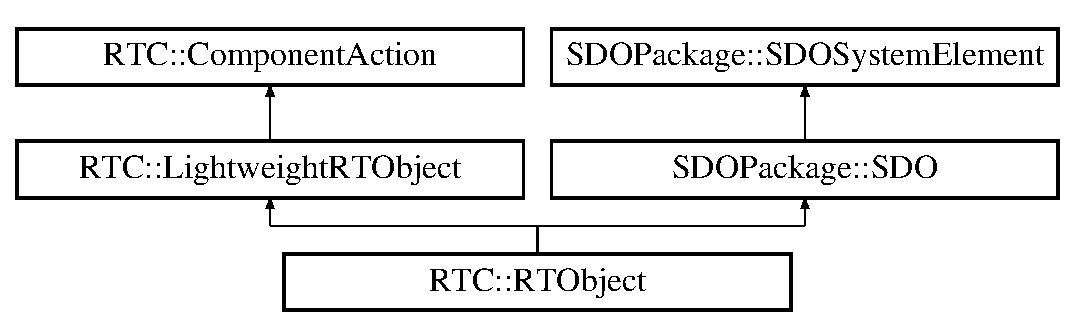
\includegraphics[height=3cm]{interfaceRTC_1_1RTObject}
\end{center}
\end{figure}
\subsection*{Public �᥽�å�}
\begin{CompactItemize}
\item 
{\bf Component\-Profile} {\bf get\_\-component\_\-profile} ()
\item 
{\bf Port\-List} {\bf get\_\-ports} ()
\item 
{\bf Execution\-Context\-Service\-List} {\bf get\_\-execution\_\-context\_\-services} ()
\item 
{\bf Return\-Code\_\-t} {\bf initialize} ()
\item 
{\bf Return\-Code\_\-t} {\bf finalize} ()
\item 
{\bf Return\-Code\_\-t} {\bf exit} ()
\item 
boolean {\bf is\_\-alive} ()
\item 
{\bf Execution\-Context\-List} {\bf get\_\-contexts} ()
\item 
{\bf Execution\-Context} {\bf get\_\-context} (in {\bf Unique\-Id} ec\_\-id)
\item 
{\bf Unique\-Id} {\bf attach\_\-executioncontext} (in {\bf Execution\-Context} exec\_\-context)
\item 
{\bf Return\-Code\_\-t} {\bf detach\_\-executioncontext} (in {\bf Unique\-Id} ec\_\-id)
\item 
{\bf Return\-Code\_\-t} {\bf on\_\-initialize} ()
\item 
{\bf Return\-Code\_\-t} {\bf on\_\-finalize} ()
\item 
{\bf Return\-Code\_\-t} {\bf on\_\-startup} (in {\bf Unique\-Id} ec\_\-id)
\item 
{\bf Return\-Code\_\-t} {\bf on\_\-shutdown} (in {\bf Unique\-Id} ec\_\-id)
\item 
{\bf Return\-Code\_\-t} {\bf on\_\-activated} (in {\bf Unique\-Id} ec\_\-id)
\item 
{\bf Return\-Code\_\-t} {\bf on\_\-deactivated} (in {\bf Unique\-Id} ec\_\-id)
\item 
{\bf Return\-Code\_\-t} {\bf on\_\-aborting} (in {\bf Unique\-Id} ec\_\-id)
\item 
{\bf Return\-Code\_\-t} {\bf on\_\-error} (in {\bf Unique\-Id} ec\_\-id)
\item 
{\bf Return\-Code\_\-t} {\bf on\_\-reset} (in {\bf Unique\-Id} ec\_\-id)
\item 
{\bf Unique\-Identifier} {\bf get\_\-sdo\_\-id} ()  raises (Not\-Available, Internal\-Error)
\item 
string {\bf get\_\-sdo\_\-type} ()  raises (Not\-Available, Internal\-Error)
\item 
Device\-Profile {\bf get\_\-device\_\-profile} ()  raises (Not\-Available, Internal\-Error)
\item 
{\bf Service\-Profile\-List} {\bf get\_\-service\_\-profiles} ()  raises (Not\-Available, Internal\-Error)
\item 
Service\-Profile {\bf get\_\-service\_\-profile} (in {\bf Unique\-Identifier} id)  raises (Invalid\-Parameter, Not\-Available, Internal\-Error)
\item 
SDOService {\bf get\_\-sdo\_\-service} (in {\bf Unique\-Identifier} id)  raises (Invalid\-Parameter, Not\-Available, Internal\-Error)
\item 
Configuration {\bf get\_\-configuration} ()  raises (Interface\-Not\-Implemented, Not\-Available, Internal\-Error)
\item 
Monitoring {\bf get\_\-monitoring} ()  raises (Interface\-Not\-Implemented, Not\-Available, Internal\-Error)
\item 
{\bf Organization\-List} {\bf get\_\-organizations} ()  raises (Not\-Available, Internal\-Error)
\item 
{\bf NVList} {\bf get\_\-status\_\-list} ()  raises (Not\-Available, Internal\-Error)
\item 
any {\bf get\_\-status} (in string name)  raises (Invalid\-Parameter, Not\-Available, Internal\-Error)
\item 
{\bf Organization\-List} {\bf get\_\-owned\_\-organizations} ()  raises (Not\-Available)
\end{CompactItemize}


\subsection{����}
Introspection::RTObject interface. 



\subsection{�ؿ�}
\index{RTC::RTObject@{RTC::RTObject}!attach_executioncontext@{attach\_\-executioncontext}}
\index{attach_executioncontext@{attach\_\-executioncontext}!RTC::RTObject@{RTC::RTObject}}
\subsubsection{\setlength{\rightskip}{0pt plus 5cm}{\bf Unique\-Id} RTC::Component\-Action::attach\_\-executioncontext (in {\bf Execution\-Context} {\em exec\_\-context})\hspace{0.3cm}{\tt  [inherited]}}\label{interfaceRTC_1_1ComponentAction_RTC_1_1RTObjecta9}


\index{RTC::RTObject@{RTC::RTObject}!detach_executioncontext@{detach\_\-executioncontext}}
\index{detach_executioncontext@{detach\_\-executioncontext}!RTC::RTObject@{RTC::RTObject}}
\subsubsection{\setlength{\rightskip}{0pt plus 5cm}{\bf Return\-Code\_\-t} RTC::Component\-Action::detach\_\-executioncontext (in {\bf Unique\-Id} {\em ec\_\-id})\hspace{0.3cm}{\tt  [inherited]}}\label{interfaceRTC_1_1ComponentAction_RTC_1_1RTObjecta10}


\index{RTC::RTObject@{RTC::RTObject}!exit@{exit}}
\index{exit@{exit}!RTC::RTObject@{RTC::RTObject}}
\subsubsection{\setlength{\rightskip}{0pt plus 5cm}{\bf Return\-Code\_\-t} RTC::Lightweight\-RTObject::exit ()\hspace{0.3cm}{\tt  [inherited]}}\label{interfaceRTC_1_1LightweightRTObject_RTC_1_1RTObjecta5}


\index{RTC::RTObject@{RTC::RTObject}!finalize@{finalize}}
\index{finalize@{finalize}!RTC::RTObject@{RTC::RTObject}}
\subsubsection{\setlength{\rightskip}{0pt plus 5cm}{\bf Return\-Code\_\-t} RTC::Lightweight\-RTObject::finalize ()\hspace{0.3cm}{\tt  [inherited]}}\label{interfaceRTC_1_1LightweightRTObject_RTC_1_1RTObjecta4}


\index{RTC::RTObject@{RTC::RTObject}!get_component_profile@{get\_\-component\_\-profile}}
\index{get_component_profile@{get\_\-component\_\-profile}!RTC::RTObject@{RTC::RTObject}}
\subsubsection{\setlength{\rightskip}{0pt plus 5cm}{\bf Component\-Profile} RTC::RTObject::get\_\-component\_\-profile ()}\label{interfaceRTC_1_1RTObject_RTC_1_1RTObjecta0}


\index{RTC::RTObject@{RTC::RTObject}!get_configuration@{get\_\-configuration}}
\index{get_configuration@{get\_\-configuration}!RTC::RTObject@{RTC::RTObject}}
\subsubsection{\setlength{\rightskip}{0pt plus 5cm}Configuration SDOPackage::SDO::get\_\-configuration ()  raises (Interface\-Not\-Implemented, Not\-Available, Internal\-Error)\hspace{0.3cm}{\tt  [inherited]}}\label{interfaceSDOPackage_1_1SDO_SDOPackage_1_1SDOa6}


\index{RTC::RTObject@{RTC::RTObject}!get_context@{get\_\-context}}
\index{get_context@{get\_\-context}!RTC::RTObject@{RTC::RTObject}}
\subsubsection{\setlength{\rightskip}{0pt plus 5cm}{\bf Execution\-Context} RTC::Lightweight\-RTObject::get\_\-context (in {\bf Unique\-Id} {\em ec\_\-id})\hspace{0.3cm}{\tt  [inherited]}}\label{interfaceRTC_1_1LightweightRTObject_RTC_1_1RTObjecta8}


\index{RTC::RTObject@{RTC::RTObject}!get_contexts@{get\_\-contexts}}
\index{get_contexts@{get\_\-contexts}!RTC::RTObject@{RTC::RTObject}}
\subsubsection{\setlength{\rightskip}{0pt plus 5cm}{\bf Execution\-Context\-List} RTC::Lightweight\-RTObject::get\_\-contexts ()\hspace{0.3cm}{\tt  [inherited]}}\label{interfaceRTC_1_1LightweightRTObject_RTC_1_1RTObjecta7}


\index{RTC::RTObject@{RTC::RTObject}!get_device_profile@{get\_\-device\_\-profile}}
\index{get_device_profile@{get\_\-device\_\-profile}!RTC::RTObject@{RTC::RTObject}}
\subsubsection{\setlength{\rightskip}{0pt plus 5cm}Device\-Profile SDOPackage::SDO::get\_\-device\_\-profile ()  raises (Not\-Available, Internal\-Error)\hspace{0.3cm}{\tt  [inherited]}}\label{interfaceSDOPackage_1_1SDO_SDOPackage_1_1SDOa2}


\index{RTC::RTObject@{RTC::RTObject}!get_execution_context_services@{get\_\-execution\_\-context\_\-services}}
\index{get_execution_context_services@{get\_\-execution\_\-context\_\-services}!RTC::RTObject@{RTC::RTObject}}
\subsubsection{\setlength{\rightskip}{0pt plus 5cm}{\bf Execution\-Context\-Service\-List} RTC::RTObject::get\_\-execution\_\-context\_\-services ()}\label{interfaceRTC_1_1RTObject_RTC_1_1RTObjecta2}


\index{RTC::RTObject@{RTC::RTObject}!get_monitoring@{get\_\-monitoring}}
\index{get_monitoring@{get\_\-monitoring}!RTC::RTObject@{RTC::RTObject}}
\subsubsection{\setlength{\rightskip}{0pt plus 5cm}Monitoring SDOPackage::SDO::get\_\-monitoring ()  raises (Interface\-Not\-Implemented, Not\-Available, Internal\-Error)\hspace{0.3cm}{\tt  [inherited]}}\label{interfaceSDOPackage_1_1SDO_SDOPackage_1_1SDOa7}


\index{RTC::RTObject@{RTC::RTObject}!get_organizations@{get\_\-organizations}}
\index{get_organizations@{get\_\-organizations}!RTC::RTObject@{RTC::RTObject}}
\subsubsection{\setlength{\rightskip}{0pt plus 5cm}{\bf Organization\-List} SDOPackage::SDO::get\_\-organizations ()  raises (Not\-Available, Internal\-Error)\hspace{0.3cm}{\tt  [inherited]}}\label{interfaceSDOPackage_1_1SDO_SDOPackage_1_1SDOa8}


\index{RTC::RTObject@{RTC::RTObject}!get_owned_organizations@{get\_\-owned\_\-organizations}}
\index{get_owned_organizations@{get\_\-owned\_\-organizations}!RTC::RTObject@{RTC::RTObject}}
\subsubsection{\setlength{\rightskip}{0pt plus 5cm}{\bf Organization\-List} SDOPackage::SDOSystem\-Element::get\_\-owned\_\-organizations ()  raises (Not\-Available)\hspace{0.3cm}{\tt  [inherited]}}\label{interfaceSDOPackage_1_1SDOSystemElement_SDOPackage_1_1SDOSystemElementa0}


\index{RTC::RTObject@{RTC::RTObject}!get_ports@{get\_\-ports}}
\index{get_ports@{get\_\-ports}!RTC::RTObject@{RTC::RTObject}}
\subsubsection{\setlength{\rightskip}{0pt plus 5cm}{\bf Port\-List} RTC::RTObject::get\_\-ports ()}\label{interfaceRTC_1_1RTObject_RTC_1_1RTObjecta1}


\index{RTC::RTObject@{RTC::RTObject}!get_sdo_id@{get\_\-sdo\_\-id}}
\index{get_sdo_id@{get\_\-sdo\_\-id}!RTC::RTObject@{RTC::RTObject}}
\subsubsection{\setlength{\rightskip}{0pt plus 5cm}{\bf Unique\-Identifier} SDOPackage::SDO::get\_\-sdo\_\-id ()  raises (Not\-Available, Internal\-Error)\hspace{0.3cm}{\tt  [inherited]}}\label{interfaceSDOPackage_1_1SDO_SDOPackage_1_1SDOa0}


\index{RTC::RTObject@{RTC::RTObject}!get_sdo_service@{get\_\-sdo\_\-service}}
\index{get_sdo_service@{get\_\-sdo\_\-service}!RTC::RTObject@{RTC::RTObject}}
\subsubsection{\setlength{\rightskip}{0pt plus 5cm}SDOService SDOPackage::SDO::get\_\-sdo\_\-service (in {\bf Unique\-Identifier} {\em id})  raises (Invalid\-Parameter, Not\-Available, Internal\-Error)\hspace{0.3cm}{\tt  [inherited]}}\label{interfaceSDOPackage_1_1SDO_SDOPackage_1_1SDOa5}


\index{RTC::RTObject@{RTC::RTObject}!get_sdo_type@{get\_\-sdo\_\-type}}
\index{get_sdo_type@{get\_\-sdo\_\-type}!RTC::RTObject@{RTC::RTObject}}
\subsubsection{\setlength{\rightskip}{0pt plus 5cm}string SDOPackage::SDO::get\_\-sdo\_\-type ()  raises (Not\-Available, Internal\-Error)\hspace{0.3cm}{\tt  [inherited]}}\label{interfaceSDOPackage_1_1SDO_SDOPackage_1_1SDOa1}


\index{RTC::RTObject@{RTC::RTObject}!get_service_profile@{get\_\-service\_\-profile}}
\index{get_service_profile@{get\_\-service\_\-profile}!RTC::RTObject@{RTC::RTObject}}
\subsubsection{\setlength{\rightskip}{0pt plus 5cm}Service\-Profile SDOPackage::SDO::get\_\-service\_\-profile (in {\bf Unique\-Identifier} {\em id})  raises (Invalid\-Parameter, Not\-Available, Internal\-Error)\hspace{0.3cm}{\tt  [inherited]}}\label{interfaceSDOPackage_1_1SDO_SDOPackage_1_1SDOa4}


\index{RTC::RTObject@{RTC::RTObject}!get_service_profiles@{get\_\-service\_\-profiles}}
\index{get_service_profiles@{get\_\-service\_\-profiles}!RTC::RTObject@{RTC::RTObject}}
\subsubsection{\setlength{\rightskip}{0pt plus 5cm}{\bf Service\-Profile\-List} SDOPackage::SDO::get\_\-service\_\-profiles ()  raises (Not\-Available, Internal\-Error)\hspace{0.3cm}{\tt  [inherited]}}\label{interfaceSDOPackage_1_1SDO_SDOPackage_1_1SDOa3}


\index{RTC::RTObject@{RTC::RTObject}!get_status@{get\_\-status}}
\index{get_status@{get\_\-status}!RTC::RTObject@{RTC::RTObject}}
\subsubsection{\setlength{\rightskip}{0pt plus 5cm}any SDOPackage::SDO::get\_\-status (in string {\em name})  raises (Invalid\-Parameter, Not\-Available, Internal\-Error)\hspace{0.3cm}{\tt  [inherited]}}\label{interfaceSDOPackage_1_1SDO_SDOPackage_1_1SDOa10}


\index{RTC::RTObject@{RTC::RTObject}!get_status_list@{get\_\-status\_\-list}}
\index{get_status_list@{get\_\-status\_\-list}!RTC::RTObject@{RTC::RTObject}}
\subsubsection{\setlength{\rightskip}{0pt plus 5cm}{\bf NVList} SDOPackage::SDO::get\_\-status\_\-list ()  raises (Not\-Available, Internal\-Error)\hspace{0.3cm}{\tt  [inherited]}}\label{interfaceSDOPackage_1_1SDO_SDOPackage_1_1SDOa9}


\index{RTC::RTObject@{RTC::RTObject}!initialize@{initialize}}
\index{initialize@{initialize}!RTC::RTObject@{RTC::RTObject}}
\subsubsection{\setlength{\rightskip}{0pt plus 5cm}{\bf Return\-Code\_\-t} RTC::Lightweight\-RTObject::initialize ()\hspace{0.3cm}{\tt  [inherited]}}\label{interfaceRTC_1_1LightweightRTObject_RTC_1_1RTObjecta3}


\index{RTC::RTObject@{RTC::RTObject}!is_alive@{is\_\-alive}}
\index{is_alive@{is\_\-alive}!RTC::RTObject@{RTC::RTObject}}
\subsubsection{\setlength{\rightskip}{0pt plus 5cm}boolean RTC::Lightweight\-RTObject::is\_\-alive ()\hspace{0.3cm}{\tt  [inherited]}}\label{interfaceRTC_1_1LightweightRTObject_RTC_1_1RTObjecta6}


\index{RTC::RTObject@{RTC::RTObject}!on_aborting@{on\_\-aborting}}
\index{on_aborting@{on\_\-aborting}!RTC::RTObject@{RTC::RTObject}}
\subsubsection{\setlength{\rightskip}{0pt plus 5cm}{\bf Return\-Code\_\-t} RTC::Component\-Action::on\_\-aborting (in {\bf Unique\-Id} {\em ec\_\-id})\hspace{0.3cm}{\tt  [inherited]}}\label{interfaceRTC_1_1ComponentAction_RTC_1_1RTObjecta17}


\index{RTC::RTObject@{RTC::RTObject}!on_activated@{on\_\-activated}}
\index{on_activated@{on\_\-activated}!RTC::RTObject@{RTC::RTObject}}
\subsubsection{\setlength{\rightskip}{0pt plus 5cm}{\bf Return\-Code\_\-t} RTC::Component\-Action::on\_\-activated (in {\bf Unique\-Id} {\em ec\_\-id})\hspace{0.3cm}{\tt  [inherited]}}\label{interfaceRTC_1_1ComponentAction_RTC_1_1RTObjecta15}


\index{RTC::RTObject@{RTC::RTObject}!on_deactivated@{on\_\-deactivated}}
\index{on_deactivated@{on\_\-deactivated}!RTC::RTObject@{RTC::RTObject}}
\subsubsection{\setlength{\rightskip}{0pt plus 5cm}{\bf Return\-Code\_\-t} RTC::Component\-Action::on\_\-deactivated (in {\bf Unique\-Id} {\em ec\_\-id})\hspace{0.3cm}{\tt  [inherited]}}\label{interfaceRTC_1_1ComponentAction_RTC_1_1RTObjecta16}


\index{RTC::RTObject@{RTC::RTObject}!on_error@{on\_\-error}}
\index{on_error@{on\_\-error}!RTC::RTObject@{RTC::RTObject}}
\subsubsection{\setlength{\rightskip}{0pt plus 5cm}{\bf Return\-Code\_\-t} RTC::Component\-Action::on\_\-error (in {\bf Unique\-Id} {\em ec\_\-id})\hspace{0.3cm}{\tt  [inherited]}}\label{interfaceRTC_1_1ComponentAction_RTC_1_1RTObjecta18}


\index{RTC::RTObject@{RTC::RTObject}!on_finalize@{on\_\-finalize}}
\index{on_finalize@{on\_\-finalize}!RTC::RTObject@{RTC::RTObject}}
\subsubsection{\setlength{\rightskip}{0pt plus 5cm}{\bf Return\-Code\_\-t} RTC::Component\-Action::on\_\-finalize ()\hspace{0.3cm}{\tt  [inherited]}}\label{interfaceRTC_1_1ComponentAction_RTC_1_1RTObjecta12}


\index{RTC::RTObject@{RTC::RTObject}!on_initialize@{on\_\-initialize}}
\index{on_initialize@{on\_\-initialize}!RTC::RTObject@{RTC::RTObject}}
\subsubsection{\setlength{\rightskip}{0pt plus 5cm}{\bf Return\-Code\_\-t} RTC::Component\-Action::on\_\-initialize ()\hspace{0.3cm}{\tt  [inherited]}}\label{interfaceRTC_1_1ComponentAction_RTC_1_1RTObjecta11}


\index{RTC::RTObject@{RTC::RTObject}!on_reset@{on\_\-reset}}
\index{on_reset@{on\_\-reset}!RTC::RTObject@{RTC::RTObject}}
\subsubsection{\setlength{\rightskip}{0pt plus 5cm}{\bf Return\-Code\_\-t} RTC::Component\-Action::on\_\-reset (in {\bf Unique\-Id} {\em ec\_\-id})\hspace{0.3cm}{\tt  [inherited]}}\label{interfaceRTC_1_1ComponentAction_RTC_1_1RTObjecta19}


\index{RTC::RTObject@{RTC::RTObject}!on_shutdown@{on\_\-shutdown}}
\index{on_shutdown@{on\_\-shutdown}!RTC::RTObject@{RTC::RTObject}}
\subsubsection{\setlength{\rightskip}{0pt plus 5cm}{\bf Return\-Code\_\-t} RTC::Component\-Action::on\_\-shutdown (in {\bf Unique\-Id} {\em ec\_\-id})\hspace{0.3cm}{\tt  [inherited]}}\label{interfaceRTC_1_1ComponentAction_RTC_1_1RTObjecta14}


\index{RTC::RTObject@{RTC::RTObject}!on_startup@{on\_\-startup}}
\index{on_startup@{on\_\-startup}!RTC::RTObject@{RTC::RTObject}}
\subsubsection{\setlength{\rightskip}{0pt plus 5cm}{\bf Return\-Code\_\-t} RTC::Component\-Action::on\_\-startup (in {\bf Unique\-Id} {\em ec\_\-id})\hspace{0.3cm}{\tt  [inherited]}}\label{interfaceRTC_1_1ComponentAction_RTC_1_1RTObjecta13}




���Υ��󥿥ե������������ϼ��Υե����뤫����������ޤ���:\begin{CompactItemize}
\item 
{\bf RTC.idl}\end{CompactItemize}

\section{SDOPackage::SDO Interface Reference}
\label{interfaceSDOPackage_1_1SDO}\index{SDOPackage::SDO@{SDOPackage::SDO}}
{\tt import \char`\"{}SDOPackage.idl\char`\"{};}

Inheritance diagram for SDOPackage::SDO::\begin{figure}[H]
\begin{center}
\leavevmode
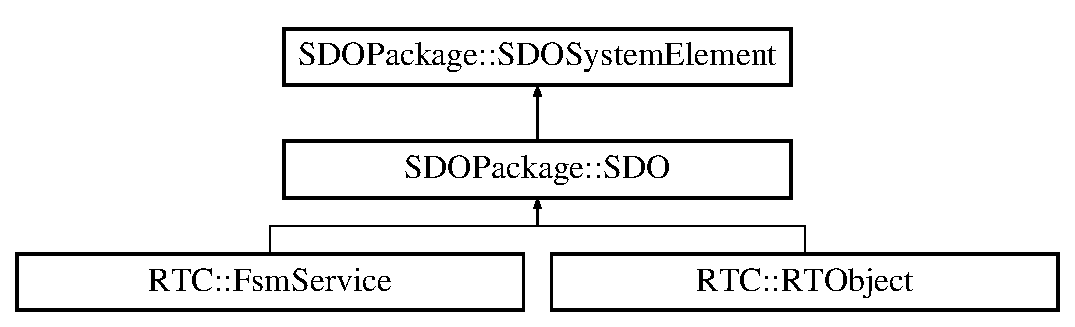
\includegraphics[height=3cm]{interfaceSDOPackage_1_1SDO}
\end{center}
\end{figure}
\subsection*{Public Member Functions}
\begin{CompactItemize}
\item 
{\bf Unique\-Identifier} {\bf get\_\-sdo\_\-id} ()  raises (Not\-Available, Internal\-Error)
\item 
string {\bf get\_\-sdo\_\-type} ()  raises (Not\-Available, Internal\-Error)
\item 
{\bf Device\-Profile} {\bf get\_\-device\_\-profile} ()  raises (Not\-Available, Internal\-Error)
\item 
{\bf Service\-Profile\-List} {\bf get\_\-service\_\-profiles} ()  raises (Not\-Available, Internal\-Error)
\item 
{\bf Service\-Profile} {\bf get\_\-service\_\-profile} (in {\bf Unique\-Identifier} id)  raises (Invalid\-Parameter, Not\-Available, Internal\-Error)
\item 
{\bf SDOService} {\bf get\_\-sdo\_\-service} (in {\bf Unique\-Identifier} id)  raises (Invalid\-Parameter, Not\-Available, Internal\-Error)
\item 
{\bf Configuration} {\bf get\_\-configuration} ()  raises (Interface\-Not\-Implemented, Not\-Available, Internal\-Error)
\item 
{\bf Monitoring} {\bf get\_\-monitoring} ()  raises (Interface\-Not\-Implemented, Not\-Available, Internal\-Error)
\item 
{\bf Organization\-List} {\bf get\_\-organizations} ()  raises (Not\-Available, Internal\-Error)
\item 
{\bf NVList} {\bf get\_\-status\_\-list} ()  raises (Not\-Available, Internal\-Error)
\item 
any {\bf get\_\-status} (in string name)  raises (Invalid\-Parameter, Not\-Available, Internal\-Error)
\item 
{\bf Organization\-List} {\bf get\_\-owned\_\-organizations} ()  raises (Not\-Available)
\end{CompactItemize}


\subsection{Member Function Documentation}
\index{SDOPackage::SDO@{SDOPackage::SDO}!get_configuration@{get\_\-configuration}}
\index{get_configuration@{get\_\-configuration}!SDOPackage::SDO@{SDOPackage::SDO}}
\subsubsection{\setlength{\rightskip}{0pt plus 5cm}{\bf Configuration} SDOPackage::SDO::get\_\-configuration ()  raises (Interface\-Not\-Implemented, Not\-Available, Internal\-Error)}\label{interfaceSDOPackage_1_1SDO_SDOPackage_1_1SDOa6}


\index{SDOPackage::SDO@{SDOPackage::SDO}!get_device_profile@{get\_\-device\_\-profile}}
\index{get_device_profile@{get\_\-device\_\-profile}!SDOPackage::SDO@{SDOPackage::SDO}}
\subsubsection{\setlength{\rightskip}{0pt plus 5cm}{\bf Device\-Profile} SDOPackage::SDO::get\_\-device\_\-profile ()  raises (Not\-Available, Internal\-Error)}\label{interfaceSDOPackage_1_1SDO_SDOPackage_1_1SDOa2}


\index{SDOPackage::SDO@{SDOPackage::SDO}!get_monitoring@{get\_\-monitoring}}
\index{get_monitoring@{get\_\-monitoring}!SDOPackage::SDO@{SDOPackage::SDO}}
\subsubsection{\setlength{\rightskip}{0pt plus 5cm}{\bf Monitoring} SDOPackage::SDO::get\_\-monitoring ()  raises (Interface\-Not\-Implemented, Not\-Available, Internal\-Error)}\label{interfaceSDOPackage_1_1SDO_SDOPackage_1_1SDOa7}


\index{SDOPackage::SDO@{SDOPackage::SDO}!get_organizations@{get\_\-organizations}}
\index{get_organizations@{get\_\-organizations}!SDOPackage::SDO@{SDOPackage::SDO}}
\subsubsection{\setlength{\rightskip}{0pt plus 5cm}{\bf Organization\-List} SDOPackage::SDO::get\_\-organizations ()  raises (Not\-Available, Internal\-Error)}\label{interfaceSDOPackage_1_1SDO_SDOPackage_1_1SDOa8}


\index{SDOPackage::SDO@{SDOPackage::SDO}!get_owned_organizations@{get\_\-owned\_\-organizations}}
\index{get_owned_organizations@{get\_\-owned\_\-organizations}!SDOPackage::SDO@{SDOPackage::SDO}}
\subsubsection{\setlength{\rightskip}{0pt plus 5cm}{\bf Organization\-List} SDOPackage::SDOSystem\-Element::get\_\-owned\_\-organizations ()  raises (Not\-Available)\hspace{0.3cm}{\tt  [inherited]}}\label{interfaceSDOPackage_1_1SDOSystemElement_SDOPackage_1_1SDOSystemElementa0}


\index{SDOPackage::SDO@{SDOPackage::SDO}!get_sdo_id@{get\_\-sdo\_\-id}}
\index{get_sdo_id@{get\_\-sdo\_\-id}!SDOPackage::SDO@{SDOPackage::SDO}}
\subsubsection{\setlength{\rightskip}{0pt plus 5cm}{\bf Unique\-Identifier} SDOPackage::SDO::get\_\-sdo\_\-id ()  raises (Not\-Available, Internal\-Error)}\label{interfaceSDOPackage_1_1SDO_SDOPackage_1_1SDOa0}


\index{SDOPackage::SDO@{SDOPackage::SDO}!get_sdo_service@{get\_\-sdo\_\-service}}
\index{get_sdo_service@{get\_\-sdo\_\-service}!SDOPackage::SDO@{SDOPackage::SDO}}
\subsubsection{\setlength{\rightskip}{0pt plus 5cm}{\bf SDOService} SDOPackage::SDO::get\_\-sdo\_\-service (in {\bf Unique\-Identifier} {\em id})  raises (Invalid\-Parameter, Not\-Available, Internal\-Error)}\label{interfaceSDOPackage_1_1SDO_SDOPackage_1_1SDOa5}


\index{SDOPackage::SDO@{SDOPackage::SDO}!get_sdo_type@{get\_\-sdo\_\-type}}
\index{get_sdo_type@{get\_\-sdo\_\-type}!SDOPackage::SDO@{SDOPackage::SDO}}
\subsubsection{\setlength{\rightskip}{0pt plus 5cm}string SDOPackage::SDO::get\_\-sdo\_\-type ()  raises (Not\-Available, Internal\-Error)}\label{interfaceSDOPackage_1_1SDO_SDOPackage_1_1SDOa1}


\index{SDOPackage::SDO@{SDOPackage::SDO}!get_service_profile@{get\_\-service\_\-profile}}
\index{get_service_profile@{get\_\-service\_\-profile}!SDOPackage::SDO@{SDOPackage::SDO}}
\subsubsection{\setlength{\rightskip}{0pt plus 5cm}{\bf Service\-Profile} SDOPackage::SDO::get\_\-service\_\-profile (in {\bf Unique\-Identifier} {\em id})  raises (Invalid\-Parameter, Not\-Available, Internal\-Error)}\label{interfaceSDOPackage_1_1SDO_SDOPackage_1_1SDOa4}


\index{SDOPackage::SDO@{SDOPackage::SDO}!get_service_profiles@{get\_\-service\_\-profiles}}
\index{get_service_profiles@{get\_\-service\_\-profiles}!SDOPackage::SDO@{SDOPackage::SDO}}
\subsubsection{\setlength{\rightskip}{0pt plus 5cm}{\bf Service\-Profile\-List} SDOPackage::SDO::get\_\-service\_\-profiles ()  raises (Not\-Available, Internal\-Error)}\label{interfaceSDOPackage_1_1SDO_SDOPackage_1_1SDOa3}


\index{SDOPackage::SDO@{SDOPackage::SDO}!get_status@{get\_\-status}}
\index{get_status@{get\_\-status}!SDOPackage::SDO@{SDOPackage::SDO}}
\subsubsection{\setlength{\rightskip}{0pt plus 5cm}any SDOPackage::SDO::get\_\-status (in string {\em name})  raises (Invalid\-Parameter, Not\-Available, Internal\-Error)}\label{interfaceSDOPackage_1_1SDO_SDOPackage_1_1SDOa10}


\index{SDOPackage::SDO@{SDOPackage::SDO}!get_status_list@{get\_\-status\_\-list}}
\index{get_status_list@{get\_\-status\_\-list}!SDOPackage::SDO@{SDOPackage::SDO}}
\subsubsection{\setlength{\rightskip}{0pt plus 5cm}{\bf NVList} SDOPackage::SDO::get\_\-status\_\-list ()  raises (Not\-Available, Internal\-Error)}\label{interfaceSDOPackage_1_1SDO_SDOPackage_1_1SDOa9}




The documentation for this interface was generated from the following file:\begin{CompactItemize}
\item 
{\bf SDOPackage.idl}\end{CompactItemize}

\section{SDOPackage::SDOService Interface Reference}
\label{interfaceSDOPackage_1_1SDOService}\index{SDOPackage::SDOService@{SDOPackage::SDOService}}
{\tt import \char`\"{}SDOPackage.idl\char`\"{};}

Inheritance diagram for SDOPackage::SDOService::\begin{figure}[H]
\begin{center}
\leavevmode
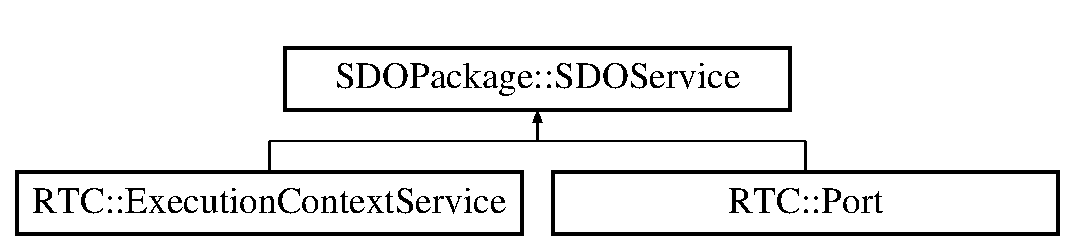
\includegraphics[height=2cm]{interfaceSDOPackage_1_1SDOService}
\end{center}
\end{figure}


The documentation for this interface was generated from the following file:\begin{CompactItemize}
\item 
{\bf SDOPackage.idl}\end{CompactItemize}

\section{SDOPackage::SDOSystem\-Element Interface Reference}
\label{interfaceSDOPackage_1_1SDOSystemElement}\index{SDOPackage::SDOSystemElement@{SDOPackage::SDOSystemElement}}
{\tt import \char`\"{}SDOPackage.idl\char`\"{};}

Inheritance diagram for SDOPackage::SDOSystem\-Element::\begin{figure}[H]
\begin{center}
\leavevmode
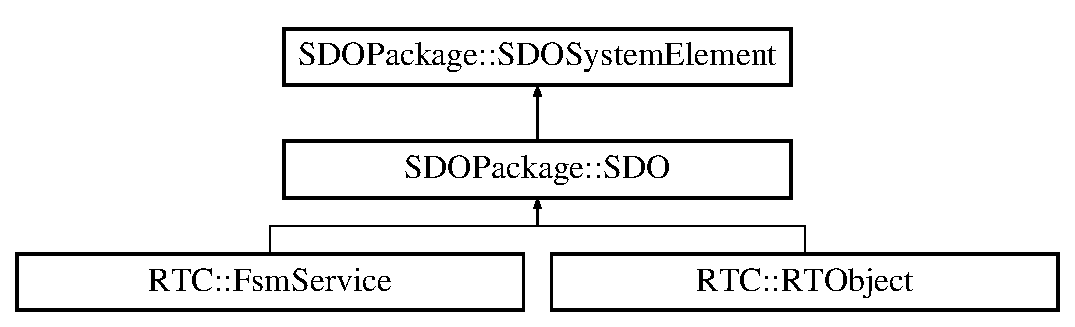
\includegraphics[height=3cm]{interfaceSDOPackage_1_1SDOSystemElement}
\end{center}
\end{figure}
\subsection*{Public Member Functions}
\begin{CompactItemize}
\item 
{\bf Organization\-List} {\bf get\_\-owned\_\-organizations} ()  raises (Not\-Available)
\end{CompactItemize}


\subsection{Detailed Description}
------- Interfaces ------- 



\subsection{Member Function Documentation}
\index{SDOPackage::SDOSystemElement@{SDOPackage::SDOSystem\-Element}!get_owned_organizations@{get\_\-owned\_\-organizations}}
\index{get_owned_organizations@{get\_\-owned\_\-organizations}!SDOPackage::SDOSystemElement@{SDOPackage::SDOSystem\-Element}}
\subsubsection{\setlength{\rightskip}{0pt plus 5cm}{\bf Organization\-List} SDOPackage::SDOSystem\-Element::get\_\-owned\_\-organizations ()  raises (Not\-Available)}\label{interfaceSDOPackage_1_1SDOSystemElement_SDOPackage_1_1SDOSystemElementa0}




The documentation for this interface was generated from the following file:\begin{CompactItemize}
\item 
{\bf SDOPackage.idl}\end{CompactItemize}

\section{��¤�� SDOPackage::Service\-Profile}
\label{structSDOPackage_1_1ServiceProfile}\index{SDOPackage::ServiceProfile@{SDOPackage::ServiceProfile}}
{\tt import \char`\"{}SDOPackage.idl\char`\"{};}

\subsection*{Public �ѿ�}
\begin{CompactItemize}
\item 
string {\bf id}
\item 
string {\bf interface\_\-type}
\item 
{\bf NVList} {\bf properties}
\item 
{\bf SDOService} {\bf service}
\end{CompactItemize}


\subsection{�ѿ�}
\index{SDOPackage::ServiceProfile@{SDOPackage::Service\-Profile}!id@{id}}
\index{id@{id}!SDOPackage::ServiceProfile@{SDOPackage::Service\-Profile}}
\subsubsection{\setlength{\rightskip}{0pt plus 5cm}string {\bf SDOPackage::Service\-Profile::id}}\label{structSDOPackage_1_1ServiceProfile_SDOPackage_1_1ServiceProfileo0}


\index{SDOPackage::ServiceProfile@{SDOPackage::Service\-Profile}!interface_type@{interface\_\-type}}
\index{interface_type@{interface\_\-type}!SDOPackage::ServiceProfile@{SDOPackage::Service\-Profile}}
\subsubsection{\setlength{\rightskip}{0pt plus 5cm}string {\bf SDOPackage::Service\-Profile::interface\_\-type}}\label{structSDOPackage_1_1ServiceProfile_SDOPackage_1_1ServiceProfileo1}


\index{SDOPackage::ServiceProfile@{SDOPackage::Service\-Profile}!properties@{properties}}
\index{properties@{properties}!SDOPackage::ServiceProfile@{SDOPackage::Service\-Profile}}
\subsubsection{\setlength{\rightskip}{0pt plus 5cm}{\bf NVList} {\bf SDOPackage::Service\-Profile::properties}}\label{structSDOPackage_1_1ServiceProfile_SDOPackage_1_1ServiceProfileo2}


\index{SDOPackage::ServiceProfile@{SDOPackage::Service\-Profile}!service@{service}}
\index{service@{service}!SDOPackage::ServiceProfile@{SDOPackage::Service\-Profile}}
\subsubsection{\setlength{\rightskip}{0pt plus 5cm}{\bf SDOService} {\bf SDOPackage::Service\-Profile::service}}\label{structSDOPackage_1_1ServiceProfile_SDOPackage_1_1ServiceProfileo3}




���ι�¤�Τ������ϼ��Υե����뤫����������ޤ���:\begin{CompactItemize}
\item 
{\bf SDOPackage.idl}\end{CompactItemize}

\section{RTC::Time Struct Reference}
\label{structRTC_1_1Time}\index{RTC::Time@{RTC::Time}}
{\tt import \char`\"{}Basic\-Data\-Type.idl\char`\"{};}

\subsection*{Public Attributes}
\begin{CompactItemize}
\item 
unsigned long {\bf sec}
\item 
unsigned long {\bf nsec}
\end{CompactItemize}


\subsection{Member Data Documentation}
\index{RTC::Time@{RTC::Time}!nsec@{nsec}}
\index{nsec@{nsec}!RTC::Time@{RTC::Time}}
\subsubsection{\setlength{\rightskip}{0pt plus 5cm}unsigned long {\bf RTC::Time::nsec}}\label{structRTC_1_1Time_RTC_1_1Timeo1}


\index{RTC::Time@{RTC::Time}!sec@{sec}}
\index{sec@{sec}!RTC::Time@{RTC::Time}}
\subsubsection{\setlength{\rightskip}{0pt plus 5cm}unsigned long {\bf RTC::Time::sec}}\label{structRTC_1_1Time_RTC_1_1Timeo0}




The documentation for this struct was generated from the following file:\begin{CompactItemize}
\item 
{\bf Basic\-Data\-Type.idl}\end{CompactItemize}

\section{RTC::Timed\-Boolean Struct Reference}
\label{structRTC_1_1TimedBoolean}\index{RTC::TimedBoolean@{RTC::TimedBoolean}}
{\tt import \char`\"{}Basic\-Data\-Type.idl\char`\"{};}

\subsection*{Public Attributes}
\begin{CompactItemize}
\item 
{\bf Time} {\bf tm}
\item 
boolean {\bf data}
\end{CompactItemize}


\subsection{Member Data Documentation}
\index{RTC::TimedBoolean@{RTC::Timed\-Boolean}!data@{data}}
\index{data@{data}!RTC::TimedBoolean@{RTC::Timed\-Boolean}}
\subsubsection{\setlength{\rightskip}{0pt plus 5cm}boolean {\bf RTC::Timed\-Boolean::data}}\label{structRTC_1_1TimedBoolean_RTC_1_1TimedBooleano1}


\index{RTC::TimedBoolean@{RTC::Timed\-Boolean}!tm@{tm}}
\index{tm@{tm}!RTC::TimedBoolean@{RTC::Timed\-Boolean}}
\subsubsection{\setlength{\rightskip}{0pt plus 5cm}{\bf Time} {\bf RTC::Timed\-Boolean::tm}}\label{structRTC_1_1TimedBoolean_RTC_1_1TimedBooleano0}




The documentation for this struct was generated from the following file:\begin{CompactItemize}
\item 
{\bf Basic\-Data\-Type.idl}\end{CompactItemize}

\section{��¤�� RTC::Timed\-Boolean\-Seq}
\label{structRTC_1_1TimedBooleanSeq}\index{RTC::TimedBooleanSeq@{RTC::TimedBooleanSeq}}
{\tt import \char`\"{}Basic\-Data\-Type.idl\char`\"{};}

\subsection*{Public �ѿ�}
\begin{CompactItemize}
\item 
{\bf Time} {\bf tm}
\item 
sequence$<$ boolean $>$ {\bf data}
\end{CompactItemize}


\subsection{�ѿ�}
\index{RTC::TimedBooleanSeq@{RTC::Timed\-Boolean\-Seq}!data@{data}}
\index{data@{data}!RTC::TimedBooleanSeq@{RTC::Timed\-Boolean\-Seq}}
\subsubsection{\setlength{\rightskip}{0pt plus 5cm}sequence$<$boolean$>$ {\bf RTC::Timed\-Boolean\-Seq::data}}\label{structRTC_1_1TimedBooleanSeq_RTC_1_1TimedBooleanSeqo1}


\index{RTC::TimedBooleanSeq@{RTC::Timed\-Boolean\-Seq}!tm@{tm}}
\index{tm@{tm}!RTC::TimedBooleanSeq@{RTC::Timed\-Boolean\-Seq}}
\subsubsection{\setlength{\rightskip}{0pt plus 5cm}{\bf Time} {\bf RTC::Timed\-Boolean\-Seq::tm}}\label{structRTC_1_1TimedBooleanSeq_RTC_1_1TimedBooleanSeqo0}




���ι�¤�Τ������ϼ��Υե����뤫����������ޤ���:\begin{CompactItemize}
\item 
{\bf Basic\-Data\-Type.idl}\end{CompactItemize}

\section{RTC::Timed\-Char Struct Reference}
\label{structRTC_1_1TimedChar}\index{RTC::TimedChar@{RTC::TimedChar}}
{\tt import \char`\"{}Basic\-Data\-Type.idl\char`\"{};}

\subsection*{Public Attributes}
\begin{CompactItemize}
\item 
{\bf Time} {\bf tm}
\item 
char {\bf data}
\end{CompactItemize}


\subsection{Member Data Documentation}
\index{RTC::TimedChar@{RTC::Timed\-Char}!data@{data}}
\index{data@{data}!RTC::TimedChar@{RTC::Timed\-Char}}
\subsubsection{\setlength{\rightskip}{0pt plus 5cm}char {\bf RTC::Timed\-Char::data}}\label{structRTC_1_1TimedChar_RTC_1_1TimedCharo1}


\index{RTC::TimedChar@{RTC::Timed\-Char}!tm@{tm}}
\index{tm@{tm}!RTC::TimedChar@{RTC::Timed\-Char}}
\subsubsection{\setlength{\rightskip}{0pt plus 5cm}{\bf Time} {\bf RTC::Timed\-Char::tm}}\label{structRTC_1_1TimedChar_RTC_1_1TimedCharo0}




The documentation for this struct was generated from the following file:\begin{CompactItemize}
\item 
{\bf Basic\-Data\-Type.idl}\end{CompactItemize}

\section{RTC::Timed\-Char\-Seq Struct Reference}
\label{structRTC_1_1TimedCharSeq}\index{RTC::TimedCharSeq@{RTC::TimedCharSeq}}
{\tt import \char`\"{}Basic\-Data\-Type.idl\char`\"{};}

\subsection*{Public Attributes}
\begin{CompactItemize}
\item 
{\bf Time} {\bf tm}
\item 
sequence$<$ char $>$ {\bf data}
\end{CompactItemize}


\subsection{Member Data Documentation}
\index{RTC::TimedCharSeq@{RTC::Timed\-Char\-Seq}!data@{data}}
\index{data@{data}!RTC::TimedCharSeq@{RTC::Timed\-Char\-Seq}}
\subsubsection{\setlength{\rightskip}{0pt plus 5cm}sequence$<$char$>$ {\bf RTC::Timed\-Char\-Seq::data}}\label{structRTC_1_1TimedCharSeq_RTC_1_1TimedCharSeqo1}


\index{RTC::TimedCharSeq@{RTC::Timed\-Char\-Seq}!tm@{tm}}
\index{tm@{tm}!RTC::TimedCharSeq@{RTC::Timed\-Char\-Seq}}
\subsubsection{\setlength{\rightskip}{0pt plus 5cm}{\bf Time} {\bf RTC::Timed\-Char\-Seq::tm}}\label{structRTC_1_1TimedCharSeq_RTC_1_1TimedCharSeqo0}




The documentation for this struct was generated from the following file:\begin{CompactItemize}
\item 
{\bf Basic\-Data\-Type.idl}\end{CompactItemize}

\section{��¤�� RTC::Timed\-Double}
\label{structRTC_1_1TimedDouble}\index{RTC::TimedDouble@{RTC::TimedDouble}}
{\tt import \char`\"{}Basic\-Data\-Type.idl\char`\"{};}

\subsection*{Public �ѿ�}
\begin{CompactItemize}
\item 
{\bf Time} {\bf tm}
\item 
double {\bf data}
\end{CompactItemize}


\subsection{�ѿ�}
\index{RTC::TimedDouble@{RTC::Timed\-Double}!data@{data}}
\index{data@{data}!RTC::TimedDouble@{RTC::Timed\-Double}}
\subsubsection{\setlength{\rightskip}{0pt plus 5cm}double {\bf RTC::Timed\-Double::data}}\label{structRTC_1_1TimedDouble_RTC_1_1TimedDoubleo1}


\index{RTC::TimedDouble@{RTC::Timed\-Double}!tm@{tm}}
\index{tm@{tm}!RTC::TimedDouble@{RTC::Timed\-Double}}
\subsubsection{\setlength{\rightskip}{0pt plus 5cm}{\bf Time} {\bf RTC::Timed\-Double::tm}}\label{structRTC_1_1TimedDouble_RTC_1_1TimedDoubleo0}




���ι�¤�Τ������ϼ��Υե����뤫����������ޤ���:\begin{CompactItemize}
\item 
{\bf Basic\-Data\-Type.idl}\end{CompactItemize}

\section{RTC::Timed\-Double\-Seq Struct Reference}
\label{structRTC_1_1TimedDoubleSeq}\index{RTC::TimedDoubleSeq@{RTC::TimedDoubleSeq}}
{\tt import \char`\"{}Basic\-Data\-Type.idl\char`\"{};}

\subsection*{Public Attributes}
\begin{CompactItemize}
\item 
{\bf Time} {\bf tm}
\item 
sequence$<$ double $>$ {\bf data}
\end{CompactItemize}


\subsection{Member Data Documentation}
\index{RTC::TimedDoubleSeq@{RTC::Timed\-Double\-Seq}!data@{data}}
\index{data@{data}!RTC::TimedDoubleSeq@{RTC::Timed\-Double\-Seq}}
\subsubsection{\setlength{\rightskip}{0pt plus 5cm}sequence$<$double$>$ {\bf RTC::Timed\-Double\-Seq::data}}\label{structRTC_1_1TimedDoubleSeq_RTC_1_1TimedDoubleSeqo1}


\index{RTC::TimedDoubleSeq@{RTC::Timed\-Double\-Seq}!tm@{tm}}
\index{tm@{tm}!RTC::TimedDoubleSeq@{RTC::Timed\-Double\-Seq}}
\subsubsection{\setlength{\rightskip}{0pt plus 5cm}{\bf Time} {\bf RTC::Timed\-Double\-Seq::tm}}\label{structRTC_1_1TimedDoubleSeq_RTC_1_1TimedDoubleSeqo0}




The documentation for this struct was generated from the following file:\begin{CompactItemize}
\item 
{\bf Basic\-Data\-Type.idl}\end{CompactItemize}

\section{��¤�� RTC::Timed\-Float}
\label{structRTC_1_1TimedFloat}\index{RTC::TimedFloat@{RTC::TimedFloat}}
{\tt import \char`\"{}Basic\-Data\-Type.idl\char`\"{};}

\subsection*{Public �ѿ�}
\begin{CompactItemize}
\item 
{\bf Time} {\bf tm}
\item 
float {\bf data}
\end{CompactItemize}


\subsection{�ѿ�}
\index{RTC::TimedFloat@{RTC::Timed\-Float}!data@{data}}
\index{data@{data}!RTC::TimedFloat@{RTC::Timed\-Float}}
\subsubsection{\setlength{\rightskip}{0pt plus 5cm}float {\bf RTC::Timed\-Float::data}}\label{structRTC_1_1TimedFloat_RTC_1_1TimedFloato1}


\index{RTC::TimedFloat@{RTC::Timed\-Float}!tm@{tm}}
\index{tm@{tm}!RTC::TimedFloat@{RTC::Timed\-Float}}
\subsubsection{\setlength{\rightskip}{0pt plus 5cm}{\bf Time} {\bf RTC::Timed\-Float::tm}}\label{structRTC_1_1TimedFloat_RTC_1_1TimedFloato0}




���ι�¤�Τ������ϼ��Υե����뤫����������ޤ���:\begin{CompactItemize}
\item 
{\bf Basic\-Data\-Type.idl}\end{CompactItemize}

\section{��¤�� RTC::Timed\-Float\-Seq}
\label{structRTC_1_1TimedFloatSeq}\index{RTC::TimedFloatSeq@{RTC::TimedFloatSeq}}
{\tt import \char`\"{}Basic\-Data\-Type.idl\char`\"{};}

\subsection*{Public �ѿ�}
\begin{CompactItemize}
\item 
{\bf Time} {\bf tm}
\item 
sequence$<$ float $>$ {\bf data}
\end{CompactItemize}


\subsection{�ѿ�}
\index{RTC::TimedFloatSeq@{RTC::Timed\-Float\-Seq}!data@{data}}
\index{data@{data}!RTC::TimedFloatSeq@{RTC::Timed\-Float\-Seq}}
\subsubsection{\setlength{\rightskip}{0pt plus 5cm}sequence$<$float$>$ {\bf RTC::Timed\-Float\-Seq::data}}\label{structRTC_1_1TimedFloatSeq_RTC_1_1TimedFloatSeqo1}


\index{RTC::TimedFloatSeq@{RTC::Timed\-Float\-Seq}!tm@{tm}}
\index{tm@{tm}!RTC::TimedFloatSeq@{RTC::Timed\-Float\-Seq}}
\subsubsection{\setlength{\rightskip}{0pt plus 5cm}{\bf Time} {\bf RTC::Timed\-Float\-Seq::tm}}\label{structRTC_1_1TimedFloatSeq_RTC_1_1TimedFloatSeqo0}




���ι�¤�Τ������ϼ��Υե����뤫����������ޤ���:\begin{CompactItemize}
\item 
{\bf Basic\-Data\-Type.idl}\end{CompactItemize}

\section{RTC::Timed\-Long Struct Reference}
\label{structRTC_1_1TimedLong}\index{RTC::TimedLong@{RTC::TimedLong}}
{\tt import \char`\"{}Basic\-Data\-Type.idl\char`\"{};}

\subsection*{Public Attributes}
\begin{CompactItemize}
\item 
{\bf Time} {\bf tm}
\item 
long {\bf data}
\end{CompactItemize}


\subsection{Member Data Documentation}
\index{RTC::TimedLong@{RTC::Timed\-Long}!data@{data}}
\index{data@{data}!RTC::TimedLong@{RTC::Timed\-Long}}
\subsubsection{\setlength{\rightskip}{0pt plus 5cm}long {\bf RTC::Timed\-Long::data}}\label{structRTC_1_1TimedLong_RTC_1_1TimedLongo1}


\index{RTC::TimedLong@{RTC::Timed\-Long}!tm@{tm}}
\index{tm@{tm}!RTC::TimedLong@{RTC::Timed\-Long}}
\subsubsection{\setlength{\rightskip}{0pt plus 5cm}{\bf Time} {\bf RTC::Timed\-Long::tm}}\label{structRTC_1_1TimedLong_RTC_1_1TimedLongo0}




The documentation for this struct was generated from the following file:\begin{CompactItemize}
\item 
{\bf Basic\-Data\-Type.idl}\end{CompactItemize}

\section{��¤�� RTC::Timed\-Long\-Seq}
\label{structRTC_1_1TimedLongSeq}\index{RTC::TimedLongSeq@{RTC::TimedLongSeq}}
{\tt import \char`\"{}Basic\-Data\-Type.idl\char`\"{};}

\subsection*{Public �ѿ�}
\begin{CompactItemize}
\item 
{\bf Time} {\bf tm}
\item 
sequence$<$ long $>$ {\bf data}
\end{CompactItemize}


\subsection{�ѿ�}
\index{RTC::TimedLongSeq@{RTC::Timed\-Long\-Seq}!data@{data}}
\index{data@{data}!RTC::TimedLongSeq@{RTC::Timed\-Long\-Seq}}
\subsubsection{\setlength{\rightskip}{0pt plus 5cm}sequence$<$long$>$ {\bf RTC::Timed\-Long\-Seq::data}}\label{structRTC_1_1TimedLongSeq_RTC_1_1TimedLongSeqo1}


\index{RTC::TimedLongSeq@{RTC::Timed\-Long\-Seq}!tm@{tm}}
\index{tm@{tm}!RTC::TimedLongSeq@{RTC::Timed\-Long\-Seq}}
\subsubsection{\setlength{\rightskip}{0pt plus 5cm}{\bf Time} {\bf RTC::Timed\-Long\-Seq::tm}}\label{structRTC_1_1TimedLongSeq_RTC_1_1TimedLongSeqo0}




���ι�¤�Τ������ϼ��Υե����뤫����������ޤ���:\begin{CompactItemize}
\item 
{\bf Basic\-Data\-Type.idl}\end{CompactItemize}

\section{RTC::Timed\-Octet Struct Reference}
\label{structRTC_1_1TimedOctet}\index{RTC::TimedOctet@{RTC::TimedOctet}}
{\tt import \char`\"{}Basic\-Data\-Type.idl\char`\"{};}

\subsection*{Public Attributes}
\begin{CompactItemize}
\item 
{\bf Time} {\bf tm}
\item 
octet {\bf data}
\end{CompactItemize}


\subsection{Member Data Documentation}
\index{RTC::TimedOctet@{RTC::Timed\-Octet}!data@{data}}
\index{data@{data}!RTC::TimedOctet@{RTC::Timed\-Octet}}
\subsubsection{\setlength{\rightskip}{0pt plus 5cm}octet {\bf RTC::Timed\-Octet::data}}\label{structRTC_1_1TimedOctet_RTC_1_1TimedOcteto1}


\index{RTC::TimedOctet@{RTC::Timed\-Octet}!tm@{tm}}
\index{tm@{tm}!RTC::TimedOctet@{RTC::Timed\-Octet}}
\subsubsection{\setlength{\rightskip}{0pt plus 5cm}{\bf Time} {\bf RTC::Timed\-Octet::tm}}\label{structRTC_1_1TimedOctet_RTC_1_1TimedOcteto0}




The documentation for this struct was generated from the following file:\begin{CompactItemize}
\item 
{\bf Basic\-Data\-Type.idl}\end{CompactItemize}

\section{��¤�� RTC::Timed\-Octet\-Seq}
\label{structRTC_1_1TimedOctetSeq}\index{RTC::TimedOctetSeq@{RTC::TimedOctetSeq}}
{\tt import \char`\"{}Basic\-Data\-Type.idl\char`\"{};}

\subsection*{Public �ѿ�}
\begin{CompactItemize}
\item 
{\bf Time} {\bf tm}
\item 
sequence$<$ octet $>$ {\bf data}
\end{CompactItemize}


\subsection{�ѿ�}
\index{RTC::TimedOctetSeq@{RTC::Timed\-Octet\-Seq}!data@{data}}
\index{data@{data}!RTC::TimedOctetSeq@{RTC::Timed\-Octet\-Seq}}
\subsubsection{\setlength{\rightskip}{0pt plus 5cm}sequence$<$octet$>$ {\bf RTC::Timed\-Octet\-Seq::data}}\label{structRTC_1_1TimedOctetSeq_RTC_1_1TimedOctetSeqo1}


\index{RTC::TimedOctetSeq@{RTC::Timed\-Octet\-Seq}!tm@{tm}}
\index{tm@{tm}!RTC::TimedOctetSeq@{RTC::Timed\-Octet\-Seq}}
\subsubsection{\setlength{\rightskip}{0pt plus 5cm}{\bf Time} {\bf RTC::Timed\-Octet\-Seq::tm}}\label{structRTC_1_1TimedOctetSeq_RTC_1_1TimedOctetSeqo0}




���ι�¤�Τ������ϼ��Υե����뤫����������ޤ���:\begin{CompactItemize}
\item 
{\bf Basic\-Data\-Type.idl}\end{CompactItemize}

\section{��¤�� RTC::Timed\-Short}
\label{structRTC_1_1TimedShort}\index{RTC::TimedShort@{RTC::TimedShort}}
{\tt import \char`\"{}Basic\-Data\-Type.idl\char`\"{};}

\subsection*{Public �ѿ�}
\begin{CompactItemize}
\item 
{\bf Time} {\bf tm}
\item 
short {\bf data}
\end{CompactItemize}


\subsection{�ѿ�}
\index{RTC::TimedShort@{RTC::Timed\-Short}!data@{data}}
\index{data@{data}!RTC::TimedShort@{RTC::Timed\-Short}}
\subsubsection{\setlength{\rightskip}{0pt plus 5cm}short {\bf RTC::Timed\-Short::data}}\label{structRTC_1_1TimedShort_RTC_1_1TimedShorto1}


\index{RTC::TimedShort@{RTC::Timed\-Short}!tm@{tm}}
\index{tm@{tm}!RTC::TimedShort@{RTC::Timed\-Short}}
\subsubsection{\setlength{\rightskip}{0pt plus 5cm}{\bf Time} {\bf RTC::Timed\-Short::tm}}\label{structRTC_1_1TimedShort_RTC_1_1TimedShorto0}




���ι�¤�Τ������ϼ��Υե����뤫����������ޤ���:\begin{CompactItemize}
\item 
{\bf Basic\-Data\-Type.idl}\end{CompactItemize}

\section{RTC::Timed\-Short\-Seq Struct Reference}
\label{structRTC_1_1TimedShortSeq}\index{RTC::TimedShortSeq@{RTC::TimedShortSeq}}
{\tt import \char`\"{}Basic\-Data\-Type.idl\char`\"{};}

\subsection*{Public Attributes}
\begin{CompactItemize}
\item 
{\bf Time} {\bf tm}
\item 
sequence$<$ short $>$ {\bf data}
\end{CompactItemize}


\subsection{Detailed Description}
Sequence data type 



\subsection{Member Data Documentation}
\index{RTC::TimedShortSeq@{RTC::Timed\-Short\-Seq}!data@{data}}
\index{data@{data}!RTC::TimedShortSeq@{RTC::Timed\-Short\-Seq}}
\subsubsection{\setlength{\rightskip}{0pt plus 5cm}sequence$<$short$>$ {\bf RTC::Timed\-Short\-Seq::data}}\label{structRTC_1_1TimedShortSeq_RTC_1_1TimedShortSeqo1}


\index{RTC::TimedShortSeq@{RTC::Timed\-Short\-Seq}!tm@{tm}}
\index{tm@{tm}!RTC::TimedShortSeq@{RTC::Timed\-Short\-Seq}}
\subsubsection{\setlength{\rightskip}{0pt plus 5cm}{\bf Time} {\bf RTC::Timed\-Short\-Seq::tm}}\label{structRTC_1_1TimedShortSeq_RTC_1_1TimedShortSeqo0}




The documentation for this struct was generated from the following file:\begin{CompactItemize}
\item 
{\bf Basic\-Data\-Type.idl}\end{CompactItemize}

\section{RTC::Timed\-State Struct Reference}
\label{structRTC_1_1TimedState}\index{RTC::TimedState@{RTC::TimedState}}
{\tt import \char`\"{}Basic\-Data\-Type.idl\char`\"{};}

\subsection*{Public Attributes}
\begin{CompactItemize}
\item 
{\bf Time} {\bf tm}
\item 
short {\bf data}
\end{CompactItemize}


\subsection{Member Data Documentation}
\index{RTC::TimedState@{RTC::Timed\-State}!data@{data}}
\index{data@{data}!RTC::TimedState@{RTC::Timed\-State}}
\subsubsection{\setlength{\rightskip}{0pt plus 5cm}short {\bf RTC::Timed\-State::data}}\label{structRTC_1_1TimedState_RTC_1_1TimedStateo1}


\index{RTC::TimedState@{RTC::Timed\-State}!tm@{tm}}
\index{tm@{tm}!RTC::TimedState@{RTC::Timed\-State}}
\subsubsection{\setlength{\rightskip}{0pt plus 5cm}{\bf Time} {\bf RTC::Timed\-State::tm}}\label{structRTC_1_1TimedState_RTC_1_1TimedStateo0}




The documentation for this struct was generated from the following file:\begin{CompactItemize}
\item 
{\bf Basic\-Data\-Type.idl}\end{CompactItemize}

\section{RTC::Timed\-String Struct Reference}
\label{structRTC_1_1TimedString}\index{RTC::TimedString@{RTC::TimedString}}
{\tt import \char`\"{}Basic\-Data\-Type.idl\char`\"{};}

\subsection*{Public Attributes}
\begin{CompactItemize}
\item 
{\bf Time} {\bf tm}
\item 
string {\bf data}
\end{CompactItemize}


\subsection{Member Data Documentation}
\index{RTC::TimedString@{RTC::Timed\-String}!data@{data}}
\index{data@{data}!RTC::TimedString@{RTC::Timed\-String}}
\subsubsection{\setlength{\rightskip}{0pt plus 5cm}string {\bf RTC::Timed\-String::data}}\label{structRTC_1_1TimedString_RTC_1_1TimedStringo1}


\index{RTC::TimedString@{RTC::Timed\-String}!tm@{tm}}
\index{tm@{tm}!RTC::TimedString@{RTC::Timed\-String}}
\subsubsection{\setlength{\rightskip}{0pt plus 5cm}{\bf Time} {\bf RTC::Timed\-String::tm}}\label{structRTC_1_1TimedString_RTC_1_1TimedStringo0}




The documentation for this struct was generated from the following file:\begin{CompactItemize}
\item 
{\bf Basic\-Data\-Type.idl}\end{CompactItemize}

\section{RTC::Timed\-String\-Seq Struct Reference}
\label{structRTC_1_1TimedStringSeq}\index{RTC::TimedStringSeq@{RTC::TimedStringSeq}}
{\tt import \char`\"{}Basic\-Data\-Type.idl\char`\"{};}

\subsection*{Public Attributes}
\begin{CompactItemize}
\item 
{\bf Time} {\bf tm}
\item 
sequence$<$ string $>$ {\bf data}
\end{CompactItemize}


\subsection{Member Data Documentation}
\index{RTC::TimedStringSeq@{RTC::Timed\-String\-Seq}!data@{data}}
\index{data@{data}!RTC::TimedStringSeq@{RTC::Timed\-String\-Seq}}
\subsubsection{\setlength{\rightskip}{0pt plus 5cm}sequence$<$string$>$ {\bf RTC::Timed\-String\-Seq::data}}\label{structRTC_1_1TimedStringSeq_RTC_1_1TimedStringSeqo1}


\index{RTC::TimedStringSeq@{RTC::Timed\-String\-Seq}!tm@{tm}}
\index{tm@{tm}!RTC::TimedStringSeq@{RTC::Timed\-String\-Seq}}
\subsubsection{\setlength{\rightskip}{0pt plus 5cm}{\bf Time} {\bf RTC::Timed\-String\-Seq::tm}}\label{structRTC_1_1TimedStringSeq_RTC_1_1TimedStringSeqo0}




The documentation for this struct was generated from the following file:\begin{CompactItemize}
\item 
{\bf Basic\-Data\-Type.idl}\end{CompactItemize}

\section{��¤�� RTC::Timed\-ULong}
\label{structRTC_1_1TimedULong}\index{RTC::TimedULong@{RTC::TimedULong}}
{\tt import \char`\"{}Basic\-Data\-Type.idl\char`\"{};}

\subsection*{Public �ѿ�}
\begin{CompactItemize}
\item 
{\bf Time} {\bf tm}
\item 
unsigned long {\bf data}
\end{CompactItemize}


\subsection{�ѿ�}
\index{RTC::TimedULong@{RTC::Timed\-ULong}!data@{data}}
\index{data@{data}!RTC::TimedULong@{RTC::Timed\-ULong}}
\subsubsection{\setlength{\rightskip}{0pt plus 5cm}unsigned long {\bf RTC::Timed\-ULong::data}}\label{structRTC_1_1TimedULong_RTC_1_1TimedULongo1}


\index{RTC::TimedULong@{RTC::Timed\-ULong}!tm@{tm}}
\index{tm@{tm}!RTC::TimedULong@{RTC::Timed\-ULong}}
\subsubsection{\setlength{\rightskip}{0pt plus 5cm}{\bf Time} {\bf RTC::Timed\-ULong::tm}}\label{structRTC_1_1TimedULong_RTC_1_1TimedULongo0}




���ι�¤�Τ������ϼ��Υե����뤫����������ޤ���:\begin{CompactItemize}
\item 
{\bf Basic\-Data\-Type.idl}\end{CompactItemize}

\section{RTC::Timed\-ULong\-Seq Struct Reference}
\label{structRTC_1_1TimedULongSeq}\index{RTC::TimedULongSeq@{RTC::TimedULongSeq}}
{\tt import \char`\"{}Basic\-Data\-Type.idl\char`\"{};}

\subsection*{Public Attributes}
\begin{CompactItemize}
\item 
{\bf Time} {\bf tm}
\item 
sequence$<$ unsigned long $>$ {\bf data}
\end{CompactItemize}


\subsection{Member Data Documentation}
\index{RTC::TimedULongSeq@{RTC::Timed\-ULong\-Seq}!data@{data}}
\index{data@{data}!RTC::TimedULongSeq@{RTC::Timed\-ULong\-Seq}}
\subsubsection{\setlength{\rightskip}{0pt plus 5cm}sequence$<$unsigned long$>$ {\bf RTC::Timed\-ULong\-Seq::data}}\label{structRTC_1_1TimedULongSeq_RTC_1_1TimedULongSeqo1}


\index{RTC::TimedULongSeq@{RTC::Timed\-ULong\-Seq}!tm@{tm}}
\index{tm@{tm}!RTC::TimedULongSeq@{RTC::Timed\-ULong\-Seq}}
\subsubsection{\setlength{\rightskip}{0pt plus 5cm}{\bf Time} {\bf RTC::Timed\-ULong\-Seq::tm}}\label{structRTC_1_1TimedULongSeq_RTC_1_1TimedULongSeqo0}




The documentation for this struct was generated from the following file:\begin{CompactItemize}
\item 
{\bf Basic\-Data\-Type.idl}\end{CompactItemize}

\section{��¤�� RTC::Timed\-UShort}
\label{structRTC_1_1TimedUShort}\index{RTC::TimedUShort@{RTC::TimedUShort}}
{\tt import \char`\"{}Basic\-Data\-Type.idl\char`\"{};}

\subsection*{Public �ѿ�}
\begin{CompactItemize}
\item 
{\bf Time} {\bf tm}
\item 
unsigned short {\bf data}
\end{CompactItemize}


\subsection{�ѿ�}
\index{RTC::TimedUShort@{RTC::Timed\-UShort}!data@{data}}
\index{data@{data}!RTC::TimedUShort@{RTC::Timed\-UShort}}
\subsubsection{\setlength{\rightskip}{0pt plus 5cm}unsigned short {\bf RTC::Timed\-UShort::data}}\label{structRTC_1_1TimedUShort_RTC_1_1TimedUShorto1}


\index{RTC::TimedUShort@{RTC::Timed\-UShort}!tm@{tm}}
\index{tm@{tm}!RTC::TimedUShort@{RTC::Timed\-UShort}}
\subsubsection{\setlength{\rightskip}{0pt plus 5cm}{\bf Time} {\bf RTC::Timed\-UShort::tm}}\label{structRTC_1_1TimedUShort_RTC_1_1TimedUShorto0}




���ι�¤�Τ������ϼ��Υե����뤫����������ޤ���:\begin{CompactItemize}
\item 
{\bf Basic\-Data\-Type.idl}\end{CompactItemize}

\section{��¤�� RTC::Timed\-UShort\-Seq}
\label{structRTC_1_1TimedUShortSeq}\index{RTC::TimedUShortSeq@{RTC::TimedUShortSeq}}
{\tt import \char`\"{}Basic\-Data\-Type.idl\char`\"{};}

\subsection*{Public �ѿ�}
\begin{CompactItemize}
\item 
{\bf Time} {\bf tm}
\item 
sequence$<$ unsigned short $>$ {\bf data}
\end{CompactItemize}


\subsection{�ѿ�}
\index{RTC::TimedUShortSeq@{RTC::Timed\-UShort\-Seq}!data@{data}}
\index{data@{data}!RTC::TimedUShortSeq@{RTC::Timed\-UShort\-Seq}}
\subsubsection{\setlength{\rightskip}{0pt plus 5cm}sequence$<$unsigned short$>$ {\bf RTC::Timed\-UShort\-Seq::data}}\label{structRTC_1_1TimedUShortSeq_RTC_1_1TimedUShortSeqo1}


\index{RTC::TimedUShortSeq@{RTC::Timed\-UShort\-Seq}!tm@{tm}}
\index{tm@{tm}!RTC::TimedUShortSeq@{RTC::Timed\-UShort\-Seq}}
\subsubsection{\setlength{\rightskip}{0pt plus 5cm}{\bf Time} {\bf RTC::Timed\-UShort\-Seq::tm}}\label{structRTC_1_1TimedUShortSeq_RTC_1_1TimedUShortSeqo0}




���ι�¤�Τ������ϼ��Υե����뤫����������ޤ���:\begin{CompactItemize}
\item 
{\bf Basic\-Data\-Type.idl}\end{CompactItemize}

\chapter{Open\-RTM File Documentation}
\section{Basic\-Data\-Type.idl}
\label{BasicDataType_8idl}\index{BasicDataType.idl@{BasicDataType.idl}}
\subsection*{�͡��ॹ�ڡ���}
\begin{CompactItemize}
\item 
namespace {\bf RTC}
\end{CompactItemize}

\section{Data\-Port.idl File Reference}
\label{DataPort_8idl}\index{DataPort.idl@{DataPort.idl}}
Data\-Port interface definition. 

\subsection*{Namespaces}
\begin{CompactItemize}
\item 
namespace {\bf RTC}
\end{CompactItemize}


\subsection{Detailed Description}
Data\-Port interface definition. 

\begin{Desc}
\item[Date:]\begin{Desc}
\item[Date]2007/01/09 15:40:14 \end{Desc}
\end{Desc}
\begin{Desc}
\item[Author:]Noriaki Ando $<${\tt n-ando@aist.go.jp}$>$\end{Desc}
Copyright (C) 2006 Noriaki Ando Task-intelligence Research Group, Intelligent Systems Research Institute, National Institute of Advanced Industrial Science and Technology (AIST), Japan

All rights reserved.

\begin{Desc}
\item[Id]{\bf Data\-Port.idl}{\rm (p.\,\pageref{DataPort_8idl})},v 1.1 2007/01/09 15:40:14 n-ando Exp \end{Desc}

\section{RTC.idl}
\label{RTC_8idl}\index{RTC.idl@{RTC.idl}}
{\tt import \char`\"{}SDOPackage.idl\char`\"{};}\par
\subsection*{�͡��ॹ�ڡ���}
\begin{CompactItemize}
\item 
namespace {\bf RTC}
\end{CompactItemize}
\subsection*{�ޥ������}
\begin{CompactItemize}
\item 
\#define {\bf UNIQUE\_\-ID\_\-TYPE\_\-NATIVE}~long
\end{CompactItemize}
\subsection*{�����}
\begin{CompactItemize}
\item 
typedef {\bf SDOPackage::Unique\-Identifier} {\bf Unique\-Identifier}
\item 
typedef {\bf SDOPackage::NVList} {\bf NVList}
\item 
typedef UNIQUE\_\-ID\_\-TYPE\_\-NATIVE {\bf Unique\-Id}
\item 
typedef sequence$<$ Mode $>$ {\bf Mode\-List}
\item 
typedef sequence$<$ Port\-Interface\-Profile $>$ {\bf Port\-Interface\-Profile\-List}
\item 
typedef sequence$<$ RTObject $>$ {\bf RTCList}
\item 
typedef sequence$<$ Connector\-Profile $>$ {\bf Connector\-Profile\-List}
\item 
typedef sequence$<$ Port\-Profile $>$ {\bf Port\-Profile\-List}
\item 
typedef sequence$<$ Execution\-Context\-Profile $>$ {\bf Execution\-Context\-Profile\-List}
\item 
typedef sequence$<$ Component\-Profile $>$ {\bf Component\-Profile\-List}
\item 
typedef sequence$<$ Execution\-Context\-Service $>$ {\bf Execution\-Context\-Service\-List}
\end{CompactItemize}
\subsection*{���}
\begin{CompactItemize}
\item 
enum {\bf Return\-Code\_\-t} \{ \par
{\bf RTC\_\-OK}, 
{\bf RTC\_\-ERROR}, 
{\bf BAD\_\-PARAMETER}, 
{\bf UNSUPPORTED}, 
\par
{\bf OUT\_\-OF\_\-RESOURCES}, 
{\bf PRECONDITION\_\-NOT\_\-MET}
 \}
\begin{CompactList}\small\item\em {\bf Lightweight\-RTC::Return\-Code\_\-t}{\rm (p.\,\pageref{namespaceRTC_a28})} enumeration. \item\end{CompactList}\item 
enum {\bf Life\-Cycle\-State} \{ {\bf INACTIVE\_\-STATE}, 
{\bf ACTIVE\_\-STATE}, 
{\bf ERROR\_\-STATE}, 
{\bf UNKNOWN\_\-STATE}
 \}
\begin{CompactList}\small\item\em {\bf Lightweight\-RTC::Life\-Cycle\-State}{\rm (p.\,\pageref{namespaceRTC_a29})} enumeration. \item\end{CompactList}\item 
enum {\bf Execution\-Kind} \{ {\bf PERIODIC}, 
{\bf EVENT\_\-DRIVEN}, 
{\bf OTHER}
 \}
\begin{CompactList}\small\item\em {\bf Lightweight\-RTC::Execution\-Kind}{\rm (p.\,\pageref{namespaceRTC_a30})} enumeration. \item\end{CompactList}\item 
enum {\bf Port\-Interface\-Polarity} \{ {\bf PROVIDED}, 
{\bf REQUIRED}
 \}
\begin{CompactList}\small\item\em {\bf Introspection::Port\-Interface\-Polarity}{\rm (p.\,\pageref{namespaceRTC_a31})} enumeration. \item\end{CompactList}\end{CompactItemize}
\subsection*{�ѿ�}
\begin{CompactItemize}
\item 
interface typedef sequence$<$ Execution\-Context $>$ {\bf Execution\-Context\-List}
\begin{CompactList}\small\item\em forward declaration of {\bf Execution\-Context}{\rm (p.\,\pageref{interfaceRTC_1_1ExecutionContext})} \item\end{CompactList}\item 
interface typedef sequence$<$ Port $>$ {\bf Port\-List}
\end{CompactItemize}


\subsection{�ޥ������}
\index{RTC.idl@{RTC.idl}!UNIQUE_ID_TYPE_NATIVE@{UNIQUE\_\-ID\_\-TYPE\_\-NATIVE}}
\index{UNIQUE_ID_TYPE_NATIVE@{UNIQUE\_\-ID\_\-TYPE\_\-NATIVE}!RTC.idl@{RTC.idl}}
\subsubsection{\setlength{\rightskip}{0pt plus 5cm}\#define UNIQUE\_\-ID\_\-TYPE\_\-NATIVE~long}\label{RTC_8idl_a0}




\subsection{�����}
\index{RTC.idl@{RTC.idl}!ComponentProfileList@{ComponentProfileList}}
\index{ComponentProfileList@{ComponentProfileList}!RTC.idl@{RTC.idl}}
\subsubsection{\setlength{\rightskip}{0pt plus 5cm}typedef sequence$<$Component\-Profile$>$ {\bf RTC::Component\-Profile\-List}}\label{namespaceRTC_file_a11}


\index{RTC.idl@{RTC.idl}!ConnectorProfileList@{ConnectorProfileList}}
\index{ConnectorProfileList@{ConnectorProfileList}!RTC.idl@{RTC.idl}}
\subsubsection{\setlength{\rightskip}{0pt plus 5cm}typedef sequence$<$Connector\-Profile$>$ {\bf RTC::Connector\-Profile\-List}}\label{namespaceRTC_file_a8}


\index{RTC.idl@{RTC.idl}!ExecutionContextProfileList@{ExecutionContextProfileList}}
\index{ExecutionContextProfileList@{ExecutionContextProfileList}!RTC.idl@{RTC.idl}}
\subsubsection{\setlength{\rightskip}{0pt plus 5cm}typedef sequence$<$Execution\-Context\-Profile$>$ {\bf RTC::Execution\-Context\-Profile\-List}}\label{namespaceRTC_file_a10}


\index{RTC.idl@{RTC.idl}!ExecutionContextServiceList@{ExecutionContextServiceList}}
\index{ExecutionContextServiceList@{ExecutionContextServiceList}!RTC.idl@{RTC.idl}}
\subsubsection{\setlength{\rightskip}{0pt plus 5cm}typedef sequence$<$Execution\-Context\-Service$>$ {\bf RTC::Execution\-Context\-Service\-List}}\label{namespaceRTC_file_a12}


\index{RTC.idl@{RTC.idl}!ModeList@{ModeList}}
\index{ModeList@{ModeList}!RTC.idl@{RTC.idl}}
\subsubsection{\setlength{\rightskip}{0pt plus 5cm}typedef sequence$<$Mode$>$ {\bf RTC::Mode\-List}}\label{namespaceRTC_file_a4}


\index{RTC.idl@{RTC.idl}!NVList@{NVList}}
\index{NVList@{NVList}!RTC.idl@{RTC.idl}}
\subsubsection{\setlength{\rightskip}{0pt plus 5cm}typedef {\bf SDOPackage::NVList} {\bf RTC::NVList}}\label{namespaceRTC_file_a1}


\index{RTC.idl@{RTC.idl}!PortInterfaceProfileList@{PortInterfaceProfileList}}
\index{PortInterfaceProfileList@{PortInterfaceProfileList}!RTC.idl@{RTC.idl}}
\subsubsection{\setlength{\rightskip}{0pt plus 5cm}typedef sequence$<$Port\-Interface\-Profile$>$ {\bf RTC::Port\-Interface\-Profile\-List}}\label{namespaceRTC_file_a5}


\index{RTC.idl@{RTC.idl}!PortProfileList@{PortProfileList}}
\index{PortProfileList@{PortProfileList}!RTC.idl@{RTC.idl}}
\subsubsection{\setlength{\rightskip}{0pt plus 5cm}typedef sequence$<$Port\-Profile$>$ {\bf RTC::Port\-Profile\-List}}\label{namespaceRTC_file_a9}


\index{RTC.idl@{RTC.idl}!RTCList@{RTCList}}
\index{RTCList@{RTCList}!RTC.idl@{RTC.idl}}
\subsubsection{\setlength{\rightskip}{0pt plus 5cm}typedef sequence$<$RTObject$>$ {\bf RTC::RTCList}}\label{namespaceRTC_file_a7}


\index{RTC.idl@{RTC.idl}!UniqueId@{UniqueId}}
\index{UniqueId@{UniqueId}!RTC.idl@{RTC.idl}}
\subsubsection{\setlength{\rightskip}{0pt plus 5cm}typedef UNIQUE\_\-ID\_\-TYPE\_\-NATIVE {\bf RTC::Unique\-Id}}\label{namespaceRTC_file_a2}


\index{RTC.idl@{RTC.idl}!UniqueIdentifier@{UniqueIdentifier}}
\index{UniqueIdentifier@{UniqueIdentifier}!RTC.idl@{RTC.idl}}
\subsubsection{\setlength{\rightskip}{0pt plus 5cm}typedef {\bf SDOPackage::Unique\-Identifier} {\bf RTC::Unique\-Identifier}}\label{namespaceRTC_file_a0}




\subsection{���}
\index{RTC.idl@{RTC.idl}!ExecutionKind@{ExecutionKind}}
\index{ExecutionKind@{ExecutionKind}!RTC.idl@{RTC.idl}}
\subsubsection{\setlength{\rightskip}{0pt plus 5cm}enum {\bf RTC::Execution\-Kind}}\label{namespaceRTC_file_a30}


{\bf Lightweight\-RTC::Execution\-Kind}{\rm (p.\,\pageref{namespaceRTC_a30})} enumeration. 

\begin{Desc}
\item[��󷿤���: ]\par
\begin{description}
\index{PERIODIC@{PERIODIC}!RTC.idl@{RTC.idl}}\index{RTC.idl@{RTC.idl}!PERIODIC@{PERIODIC}}\item[{\em 
PERIODIC\label{namespaceRTC_a30a23}
}]\index{EVENT_DRIVEN@{EVENT\_\-DRIVEN}!RTC.idl@{RTC.idl}}\index{RTC.idl@{RTC.idl}!EVENT_DRIVEN@{EVENT\_\-DRIVEN}}\item[{\em 
EVENT\_\-DRIVEN\label{namespaceRTC_a30a24}
}]\index{OTHER@{OTHER}!RTC.idl@{RTC.idl}}\index{RTC.idl@{RTC.idl}!OTHER@{OTHER}}\item[{\em 
OTHER\label{namespaceRTC_a30a25}
}]\end{description}
\end{Desc}

\index{RTC.idl@{RTC.idl}!LifeCycleState@{LifeCycleState}}
\index{LifeCycleState@{LifeCycleState}!RTC.idl@{RTC.idl}}
\subsubsection{\setlength{\rightskip}{0pt plus 5cm}enum {\bf RTC::Life\-Cycle\-State}}\label{namespaceRTC_file_a29}


{\bf Lightweight\-RTC::Life\-Cycle\-State}{\rm (p.\,\pageref{namespaceRTC_a29})} enumeration. 

\begin{Desc}
\item[��󷿤���: ]\par
\begin{description}
\index{INACTIVE_STATE@{INACTIVE\_\-STATE}!RTC.idl@{RTC.idl}}\index{RTC.idl@{RTC.idl}!INACTIVE_STATE@{INACTIVE\_\-STATE}}\item[{\em 
INACTIVE\_\-STATE\label{namespaceRTC_a29a19}
}]\index{ACTIVE_STATE@{ACTIVE\_\-STATE}!RTC.idl@{RTC.idl}}\index{RTC.idl@{RTC.idl}!ACTIVE_STATE@{ACTIVE\_\-STATE}}\item[{\em 
ACTIVE\_\-STATE\label{namespaceRTC_a29a20}
}]\index{ERROR_STATE@{ERROR\_\-STATE}!RTC.idl@{RTC.idl}}\index{RTC.idl@{RTC.idl}!ERROR_STATE@{ERROR\_\-STATE}}\item[{\em 
ERROR\_\-STATE\label{namespaceRTC_a29a21}
}]\index{UNKNOWN_STATE@{UNKNOWN\_\-STATE}!RTC.idl@{RTC.idl}}\index{RTC.idl@{RTC.idl}!UNKNOWN_STATE@{UNKNOWN\_\-STATE}}\item[{\em 
UNKNOWN\_\-STATE\label{namespaceRTC_a29a22}
}]\end{description}
\end{Desc}

\index{RTC.idl@{RTC.idl}!PortInterfacePolarity@{PortInterfacePolarity}}
\index{PortInterfacePolarity@{PortInterfacePolarity}!RTC.idl@{RTC.idl}}
\subsubsection{\setlength{\rightskip}{0pt plus 5cm}enum {\bf RTC::Port\-Interface\-Polarity}}\label{namespaceRTC_file_a31}


{\bf Introspection::Port\-Interface\-Polarity}{\rm (p.\,\pageref{namespaceRTC_a31})} enumeration. 

\begin{Desc}
\item[��󷿤���: ]\par
\begin{description}
\index{PROVIDED@{PROVIDED}!RTC.idl@{RTC.idl}}\index{RTC.idl@{RTC.idl}!PROVIDED@{PROVIDED}}\item[{\em 
PROVIDED\label{namespaceRTC_a31a26}
}]\index{REQUIRED@{REQUIRED}!RTC.idl@{RTC.idl}}\index{RTC.idl@{RTC.idl}!REQUIRED@{REQUIRED}}\item[{\em 
REQUIRED\label{namespaceRTC_a31a27}
}]\end{description}
\end{Desc}

\index{RTC.idl@{RTC.idl}!ReturnCode_t@{ReturnCode\_\-t}}
\index{ReturnCode_t@{ReturnCode\_\-t}!RTC.idl@{RTC.idl}}
\subsubsection{\setlength{\rightskip}{0pt plus 5cm}enum {\bf RTC::Return\-Code\_\-t}}\label{namespaceRTC_file_a28}


{\bf Lightweight\-RTC::Return\-Code\_\-t}{\rm (p.\,\pageref{namespaceRTC_a28})} enumeration. 

\begin{Desc}
\item[��󷿤���: ]\par
\begin{description}
\index{RTC_OK@{RTC\_\-OK}!RTC.idl@{RTC.idl}}\index{RTC.idl@{RTC.idl}!RTC_OK@{RTC\_\-OK}}\item[{\em 
RTC\_\-OK\label{namespaceRTC_a28a13}
}]\index{RTC_ERROR@{RTC\_\-ERROR}!RTC.idl@{RTC.idl}}\index{RTC.idl@{RTC.idl}!RTC_ERROR@{RTC\_\-ERROR}}\item[{\em 
RTC\_\-ERROR\label{namespaceRTC_a28a14}
}]\index{BAD_PARAMETER@{BAD\_\-PARAMETER}!RTC.idl@{RTC.idl}}\index{RTC.idl@{RTC.idl}!BAD_PARAMETER@{BAD\_\-PARAMETER}}\item[{\em 
BAD\_\-PARAMETER\label{namespaceRTC_a28a15}
}]\index{UNSUPPORTED@{UNSUPPORTED}!RTC.idl@{RTC.idl}}\index{RTC.idl@{RTC.idl}!UNSUPPORTED@{UNSUPPORTED}}\item[{\em 
UNSUPPORTED\label{namespaceRTC_a28a16}
}]\index{OUT_OF_RESOURCES@{OUT\_\-OF\_\-RESOURCES}!RTC.idl@{RTC.idl}}\index{RTC.idl@{RTC.idl}!OUT_OF_RESOURCES@{OUT\_\-OF\_\-RESOURCES}}\item[{\em 
OUT\_\-OF\_\-RESOURCES\label{namespaceRTC_a28a17}
}]\index{PRECONDITION_NOT_MET@{PRECONDITION\_\-NOT\_\-MET}!RTC.idl@{RTC.idl}}\index{RTC.idl@{RTC.idl}!PRECONDITION_NOT_MET@{PRECONDITION\_\-NOT\_\-MET}}\item[{\em 
PRECONDITION\_\-NOT\_\-MET\label{namespaceRTC_a28a18}
}]\end{description}
\end{Desc}



\subsection{�ѿ�}
\index{RTC.idl@{RTC.idl}!ExecutionContextList@{ExecutionContextList}}
\index{ExecutionContextList@{ExecutionContextList}!RTC.idl@{RTC.idl}}
\subsubsection{\setlength{\rightskip}{0pt plus 5cm}interface typedef sequence$<$Execution\-Context$>$ {\bf RTC::Execution\-Context\-List}}\label{namespaceRTC_file_a3}


forward declaration of {\bf Execution\-Context}{\rm (p.\,\pageref{interfaceRTC_1_1ExecutionContext})} 

\index{RTC.idl@{RTC.idl}!PortList@{PortList}}
\index{PortList@{PortList}!RTC.idl@{RTC.idl}}
\subsubsection{\setlength{\rightskip}{0pt plus 5cm}interface typedef sequence$<$Port$>$ {\bf RTC::Port\-List}}\label{namespaceRTC_file_a6}



\section{SDOPackage.idl}
\label{SDOPackage_8idl}\index{SDOPackage.idl@{SDOPackage.idl}}
\subsection*{�͡��ॹ�ڡ���}
\begin{CompactItemize}
\item 
namespace {\bf SDOPackage}
\end{CompactItemize}
\subsection*{�ޥ������}
\begin{CompactItemize}
\item 
\#define {\bf Type\-Code}~CORBA::Type\-Code
\item 
\#define {\bf exception\_\-body}~\{ string description; \}
\end{CompactItemize}
\subsection*{�����}
\begin{CompactItemize}
\item 
typedef sequence$<$ SDO $>$ {\bf SDOList}
\item 
typedef sequence$<$ Organization $>$ {\bf Organization\-List}
\item 
typedef string {\bf Unique\-Identifier}
\item 
typedef sequence$<$ Name\-Value $>$ {\bf NVList}
\item 
typedef sequence$<$ Parameter $>$ {\bf Parameter\-List}
\item 
typedef sequence$<$ Service\-Profile $>$ {\bf Service\-Profile\-List}
\item 
typedef sequence$<$ Configuration\-Set $>$ {\bf Configuration\-Set\-List}
\end{CompactItemize}
\subsection*{���}
\begin{CompactItemize}
\item 
enum {\bf Numeric\-Type} \{ {\bf SHORT\_\-TYPE}, 
{\bf LONG\_\-TYPE}, 
{\bf FLOAT\_\-TYPE}, 
{\bf DOUBLE\_\-TYPE}
 \}
\item 
enum {\bf Complex\-Data\-Type} \{ {\bf ENUMERATION}, 
{\bf RANGE}, 
{\bf INTERVAL}
 \}
\item 
enum {\bf Dependency\-Type} \{ {\bf OWN}, 
{\bf OWNED}, 
{\bf NO\_\-DEPENDENCY}
 \}
\end{CompactItemize}
\subsection*{�ѿ�}
\begin{CompactItemize}
\item 
interface interface interface interface interface interface typedef sequence$<$ string $>$ {\bf String\-List}
\item 
exception Not\-Available {\bf exception\_\-body}
\end{CompactItemize}


\subsection{�ޥ������}
\index{SDOPackage.idl@{SDOPackage.idl}!exception_body@{exception\_\-body}}
\index{exception_body@{exception\_\-body}!SDOPackage.idl@{SDOPackage.idl}}
\subsubsection{\setlength{\rightskip}{0pt plus 5cm}\#define {\bf exception\_\-body}~\{ string description; \}}\label{SDOPackage_8idl_a1}


CORBA specific model for SDOs \index{SDOPackage.idl@{SDOPackage.idl}!TypeCode@{TypeCode}}
\index{TypeCode@{TypeCode}!SDOPackage.idl@{SDOPackage.idl}}
\subsubsection{\setlength{\rightskip}{0pt plus 5cm}\#define Type\-Code~CORBA::Type\-Code}\label{SDOPackage_8idl_a0}




\subsection{�����}
\index{SDOPackage.idl@{SDOPackage.idl}!ConfigurationSetList@{ConfigurationSetList}}
\index{ConfigurationSetList@{ConfigurationSetList}!SDOPackage.idl@{SDOPackage.idl}}
\subsubsection{\setlength{\rightskip}{0pt plus 5cm}typedef sequence$<$Configuration\-Set$>$ {\bf SDOPackage::Configuration\-Set\-List}}\label{namespaceSDOPackage_file_a7}


\index{SDOPackage.idl@{SDOPackage.idl}!NVList@{NVList}}
\index{NVList@{NVList}!SDOPackage.idl@{SDOPackage.idl}}
\subsubsection{\setlength{\rightskip}{0pt plus 5cm}typedef sequence$<$Name\-Value$>$ {\bf SDOPackage::NVList}}\label{namespaceSDOPackage_file_a4}


\index{SDOPackage.idl@{SDOPackage.idl}!OrganizationList@{OrganizationList}}
\index{OrganizationList@{OrganizationList}!SDOPackage.idl@{SDOPackage.idl}}
\subsubsection{\setlength{\rightskip}{0pt plus 5cm}typedef sequence$<$Organization$>$ {\bf SDOPackage::Organization\-List}}\label{namespaceSDOPackage_file_a2}


\index{SDOPackage.idl@{SDOPackage.idl}!ParameterList@{ParameterList}}
\index{ParameterList@{ParameterList}!SDOPackage.idl@{SDOPackage.idl}}
\subsubsection{\setlength{\rightskip}{0pt plus 5cm}typedef sequence$<$Parameter$>$ {\bf SDOPackage::Parameter\-List}}\label{namespaceSDOPackage_file_a5}


\index{SDOPackage.idl@{SDOPackage.idl}!SDOList@{SDOList}}
\index{SDOList@{SDOList}!SDOPackage.idl@{SDOPackage.idl}}
\subsubsection{\setlength{\rightskip}{0pt plus 5cm}typedef sequence$<$SDO$>$ {\bf SDOPackage::SDOList}}\label{namespaceSDOPackage_file_a1}


\index{SDOPackage.idl@{SDOPackage.idl}!ServiceProfileList@{ServiceProfileList}}
\index{ServiceProfileList@{ServiceProfileList}!SDOPackage.idl@{SDOPackage.idl}}
\subsubsection{\setlength{\rightskip}{0pt plus 5cm}typedef sequence$<$Service\-Profile$>$ {\bf SDOPackage::Service\-Profile\-List}}\label{namespaceSDOPackage_file_a6}


\index{SDOPackage.idl@{SDOPackage.idl}!UniqueIdentifier@{UniqueIdentifier}}
\index{UniqueIdentifier@{UniqueIdentifier}!SDOPackage.idl@{SDOPackage.idl}}
\subsubsection{\setlength{\rightskip}{0pt plus 5cm}typedef string {\bf SDOPackage::Unique\-Identifier}}\label{namespaceSDOPackage_file_a3}




\subsection{���}
\index{SDOPackage.idl@{SDOPackage.idl}!ComplexDataType@{ComplexDataType}}
\index{ComplexDataType@{ComplexDataType}!SDOPackage.idl@{SDOPackage.idl}}
\subsubsection{\setlength{\rightskip}{0pt plus 5cm}enum {\bf SDOPackage::Complex\-Data\-Type}}\label{namespaceSDOPackage_file_a20}


\begin{Desc}
\item[��󷿤���: ]\par
\begin{description}
\index{ENUMERATION@{ENUMERATION}!SDOPackage.idl@{SDOPackage.idl}}\index{SDOPackage.idl@{SDOPackage.idl}!ENUMERATION@{ENUMERATION}}\item[{\em 
ENUMERATION\label{namespaceSDOPackage_a20a13}
}]\index{RANGE@{RANGE}!SDOPackage.idl@{SDOPackage.idl}}\index{SDOPackage.idl@{SDOPackage.idl}!RANGE@{RANGE}}\item[{\em 
RANGE\label{namespaceSDOPackage_a20a14}
}]\index{INTERVAL@{INTERVAL}!SDOPackage.idl@{SDOPackage.idl}}\index{SDOPackage.idl@{SDOPackage.idl}!INTERVAL@{INTERVAL}}\item[{\em 
INTERVAL\label{namespaceSDOPackage_a20a15}
}]\end{description}
\end{Desc}

\index{SDOPackage.idl@{SDOPackage.idl}!DependencyType@{DependencyType}}
\index{DependencyType@{DependencyType}!SDOPackage.idl@{SDOPackage.idl}}
\subsubsection{\setlength{\rightskip}{0pt plus 5cm}enum {\bf SDOPackage::Dependency\-Type}}\label{namespaceSDOPackage_file_a21}


\begin{Desc}
\item[��󷿤���: ]\par
\begin{description}
\index{OWN@{OWN}!SDOPackage.idl@{SDOPackage.idl}}\index{SDOPackage.idl@{SDOPackage.idl}!OWN@{OWN}}\item[{\em 
OWN\label{namespaceSDOPackage_a21a16}
}]\index{OWNED@{OWNED}!SDOPackage.idl@{SDOPackage.idl}}\index{SDOPackage.idl@{SDOPackage.idl}!OWNED@{OWNED}}\item[{\em 
OWNED\label{namespaceSDOPackage_a21a17}
}]\index{NO_DEPENDENCY@{NO\_\-DEPENDENCY}!SDOPackage.idl@{SDOPackage.idl}}\index{SDOPackage.idl@{SDOPackage.idl}!NO_DEPENDENCY@{NO\_\-DEPENDENCY}}\item[{\em 
NO\_\-DEPENDENCY\label{namespaceSDOPackage_a21a18}
}]\end{description}
\end{Desc}

\index{SDOPackage.idl@{SDOPackage.idl}!NumericType@{NumericType}}
\index{NumericType@{NumericType}!SDOPackage.idl@{SDOPackage.idl}}
\subsubsection{\setlength{\rightskip}{0pt plus 5cm}enum {\bf SDOPackage::Numeric\-Type}}\label{namespaceSDOPackage_file_a19}


\begin{Desc}
\item[��󷿤���: ]\par
\begin{description}
\index{SHORT_TYPE@{SHORT\_\-TYPE}!SDOPackage.idl@{SDOPackage.idl}}\index{SDOPackage.idl@{SDOPackage.idl}!SHORT_TYPE@{SHORT\_\-TYPE}}\item[{\em 
SHORT\_\-TYPE\label{namespaceSDOPackage_a19a9}
}]\index{LONG_TYPE@{LONG\_\-TYPE}!SDOPackage.idl@{SDOPackage.idl}}\index{SDOPackage.idl@{SDOPackage.idl}!LONG_TYPE@{LONG\_\-TYPE}}\item[{\em 
LONG\_\-TYPE\label{namespaceSDOPackage_a19a10}
}]\index{FLOAT_TYPE@{FLOAT\_\-TYPE}!SDOPackage.idl@{SDOPackage.idl}}\index{SDOPackage.idl@{SDOPackage.idl}!FLOAT_TYPE@{FLOAT\_\-TYPE}}\item[{\em 
FLOAT\_\-TYPE\label{namespaceSDOPackage_a19a11}
}]\index{DOUBLE_TYPE@{DOUBLE\_\-TYPE}!SDOPackage.idl@{SDOPackage.idl}}\index{SDOPackage.idl@{SDOPackage.idl}!DOUBLE_TYPE@{DOUBLE\_\-TYPE}}\item[{\em 
DOUBLE\_\-TYPE\label{namespaceSDOPackage_a19a12}
}]\end{description}
\end{Desc}



\subsection{�ѿ�}
\index{SDOPackage.idl@{SDOPackage.idl}!exception_body@{exception\_\-body}}
\index{exception_body@{exception\_\-body}!SDOPackage.idl@{SDOPackage.idl}}
\subsubsection{\setlength{\rightskip}{0pt plus 5cm}exception Internal\-Error {\bf SDOPackage::exception\_\-body}}\label{namespaceSDOPackage_file_a8}


------- Exceptions ------- \index{SDOPackage.idl@{SDOPackage.idl}!StringList@{StringList}}
\index{StringList@{StringList}!SDOPackage.idl@{SDOPackage.idl}}
\subsubsection{\setlength{\rightskip}{0pt plus 5cm}interface interface interface interface interface interface typedef sequence$<$string$>$ {\bf SDOPackage::String\-List}}\label{namespaceSDOPackage_file_a0}


------- Data Types ------- 
\printindex
\end{document}
